% !TEX TS-program = pdflatex
% !TEX encoding = UTF-8 Unicode

% This is a simple template for a LaTeX document using the "article" class.
% See "book", "report", "letter" for other types of document.

\documentclass[11pt]{article} % use larger type; default would be 10pt

\usepackage[utf8]{inputenc} % set input encoding (not needed with XeLaTeX)

%%% Examples of Article customizations
% These packages are optional, depending whether you want the features they provide.
% See the LaTeX Companion or other references for full information.

%%% PAGE DIMENSIONS
\usepackage{geometry} % to change the page dimensions
\geometry{a4paper} % or letterpaper (US) or a5paper or....
\geometry{margin=0.5in} % for example, change the margins to 2 inches all round
% \geometry{landscape} % set up the page for landscape
%   read geometry.pdf for detailed page layout information

\usepackage{graphicx} % support the \includegraphics command and options

% \usepackage[parfill]{parskip} % Activate to begin paragraphs with an empty line rather than an indent

%%% PACKAGES
\usepackage{booktabs} % for much better looking tables
\usepackage{array} % for better arrays (eg matrices) in maths
\usepackage{paralist} % very flexible & customisable lists (eg. enumerate/itemize, etc.)
\usepackage{verbatim} % adds environment for commenting out blocks of text & for better verbatim
\usepackage{subfig} % make it possible to include more than one captioned figure/table in a single float
% These packages are all incorporated in the memoir class to one degree or another...

%%% HEADERS & FOOTERS
\usepackage{fancyhdr} % This should be set AFTER setting up the page geometry
\pagestyle{fancy} % options: empty , plain , fancy
\renewcommand{\headrulewidth}{0pt} % customise the layout...
\lhead{}\chead{}\rhead{}
\lfoot{}\cfoot{\thepage}\rfoot{}

%%% SECTION TITLE APPEARANCE
\usepackage{sectsty}
\allsectionsfont{\sffamily\mdseries\upshape} % (See the fntguide.pdf for font help)
% (This matches ConTeXt defaults)

%%% ToC (table of contents) APPEARANCE
\usepackage[nottoc,notlof,notlot]{tocbibind} % Put the bibliography in the ToC
\usepackage[titles,subfigure]{tocloft} % Alter the style of the Table of Contents
\renewcommand{\cftsecfont}{\rmfamily\mdseries\upshape}
\renewcommand{\cftsecpagefont}{\rmfamily\mdseries\upshape} % No bold!

%%% END Article customizations

%%% The "real" document content comes below...

\title{Week 6 Assignment}
\author{Efeosa Eguavoen - 17324649}
%\date{} % Activate to display a given date or no date (if empty),
         % otherwise the current date is printed 

\begin{document}
\maketitle
\section{(i)}

\subsection{A}
\begin{figure}[h]
\centering
\subfloat[Gamma = 0]{{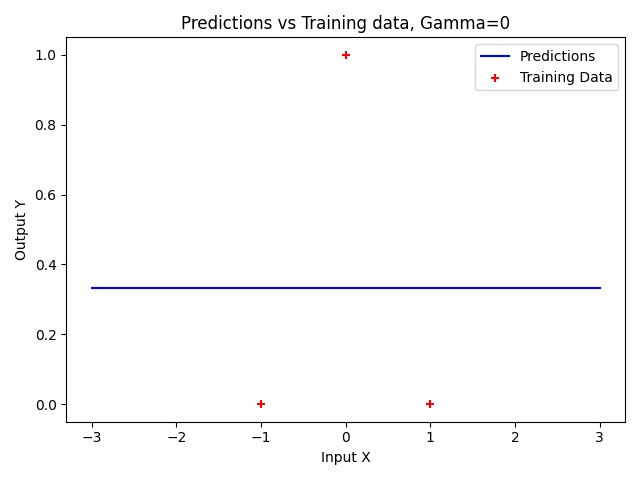
\includegraphics[width=8cm]{kn1.png}}}
\qquad
\subfloat[Gamma = 1]{{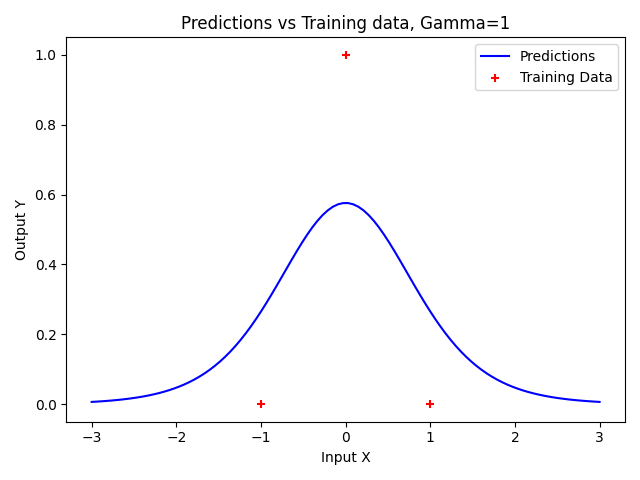
\includegraphics[width=8cm]{kn2.png}}}
\qquad
\subfloat[Gamma = 5]{{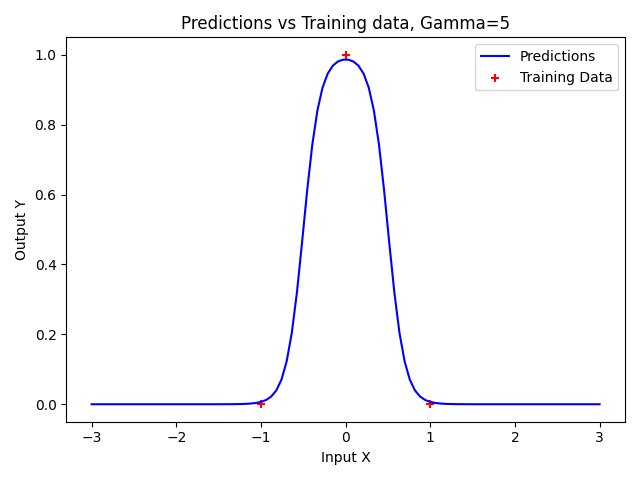
\includegraphics[width=8cm]{kn3.png}}}
\qquad
\subfloat[Gamma = 10]{{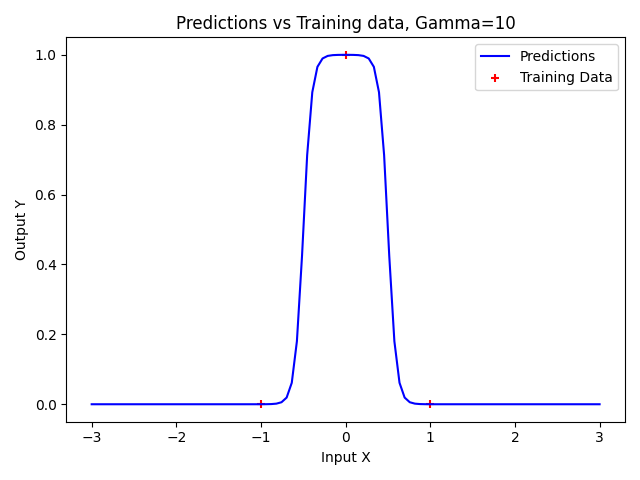
\includegraphics[width=8cm]{kn4.png}}}
\qquad
\subfloat[Gamma = 25]{{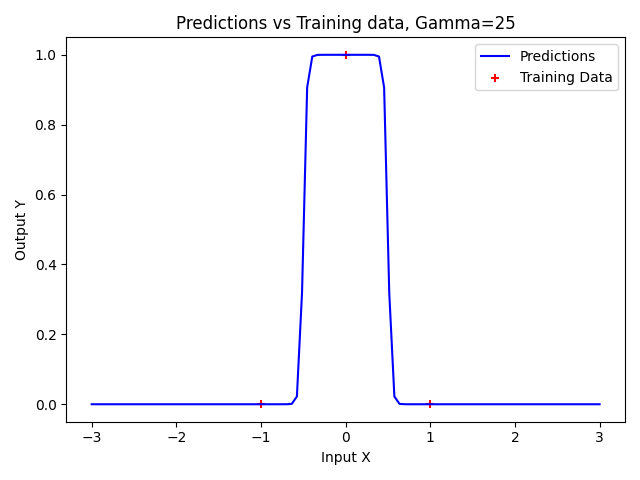
\includegraphics[width=8cm]{kn5.png}}}
\end{figure}
From the above figures we can see that as we increase gamma, our predictions fit closer to the training data,  with low values of data under-fitting the data such as when gamma = 1 and higher values of gamma confirming very closely to the data such as when gamma = 25.\\
To get the above graphs, I put the training data into a list. From there I callled KNGaus() a function I created to do all KNN Regression stuff. In this function I changed Gamma according to a list of Gamma values I had defined and then from there I built a model for each Gamma value and predicted on the grid of values to get the output. 
\begin{verbatim}
def KNGaus():
    dataframe = read_data()
    for i in range(len(gamma_Vals)):
        global gamma
        gamma = gamma_Vals[i]
        model = KNeighborsRegressor(n_neighbors=len(dataframe), weights=gaussian_kernel)
        model.fit(np.array(dataframe['x']).reshape(-1, 1), dataframe['y'])
        ys = model.predict(grid)
        plt.clf()
\end{verbatim}

\subsection{B}
From the graphs in A we can see our predictions changing as we increase the value of Gamma. This is due to fact that as we increase gamma, we decrease the rate at which the out put for our kernel grows. KNN uses the distances between a point and all other points in the data and selects the K closest examples, then sets the averages of the labels. Normally all datapoints have uniform weights but by using a Gaussian kernel, the weights of datapoints changes as they get further away from the origin datapoint, with gamma effecting how quickly this change happens. From our data we can see that low values of Gamma make the kernel decrease much slower with distance and under-fit the data, hence the slopes we see when Gamma = 1, due to more weight being on points close to the origin point. In contrast, high values of Gamma make the kernel decrease very quickly, putting less weight on points even if they're close to the origin, causing the predictions to snap towards the nearest data point such as when Gamma = 25. This also explains why when x is between -.5 and .5 we see y =1 as it's snapping towards the nearest data point. 

\subsection{C}
From the graphs below, we can see that as we change C and the Gamma, the shape of our graph alters quite considerably. Higher C values gives graphs with higher peaks and with higher gamma values influencing this also. \\ The below values represent each page of graphs hence the blocks of 5. \\ To get the graphs values, I called the kernel\_ridge function I defined. In the function I used 2 lists of values; a list of C values and Gamma values. I iterated over both lists simultaneously to get the graphs.  
\begin{verbatim}
dataframe = read_data()
    # for i in range(len(c_vals)):
    for s in range(len(gamma_Vals)):
            global gamma
            gamma = gamma_Vals[s]
            model = KernelRidge(alpha=1 / (2 * 11.102), kernel='rbf', gamma=gamma)
            model.fit(np.array(dataframe['x']).reshape(-1, 1), dataframe['y'])
            ys = model.predict(grid)
\end{verbatim}

\begin{figure}[h]
\centering
\subfloat[Gamma = 0, C = 0.1]{{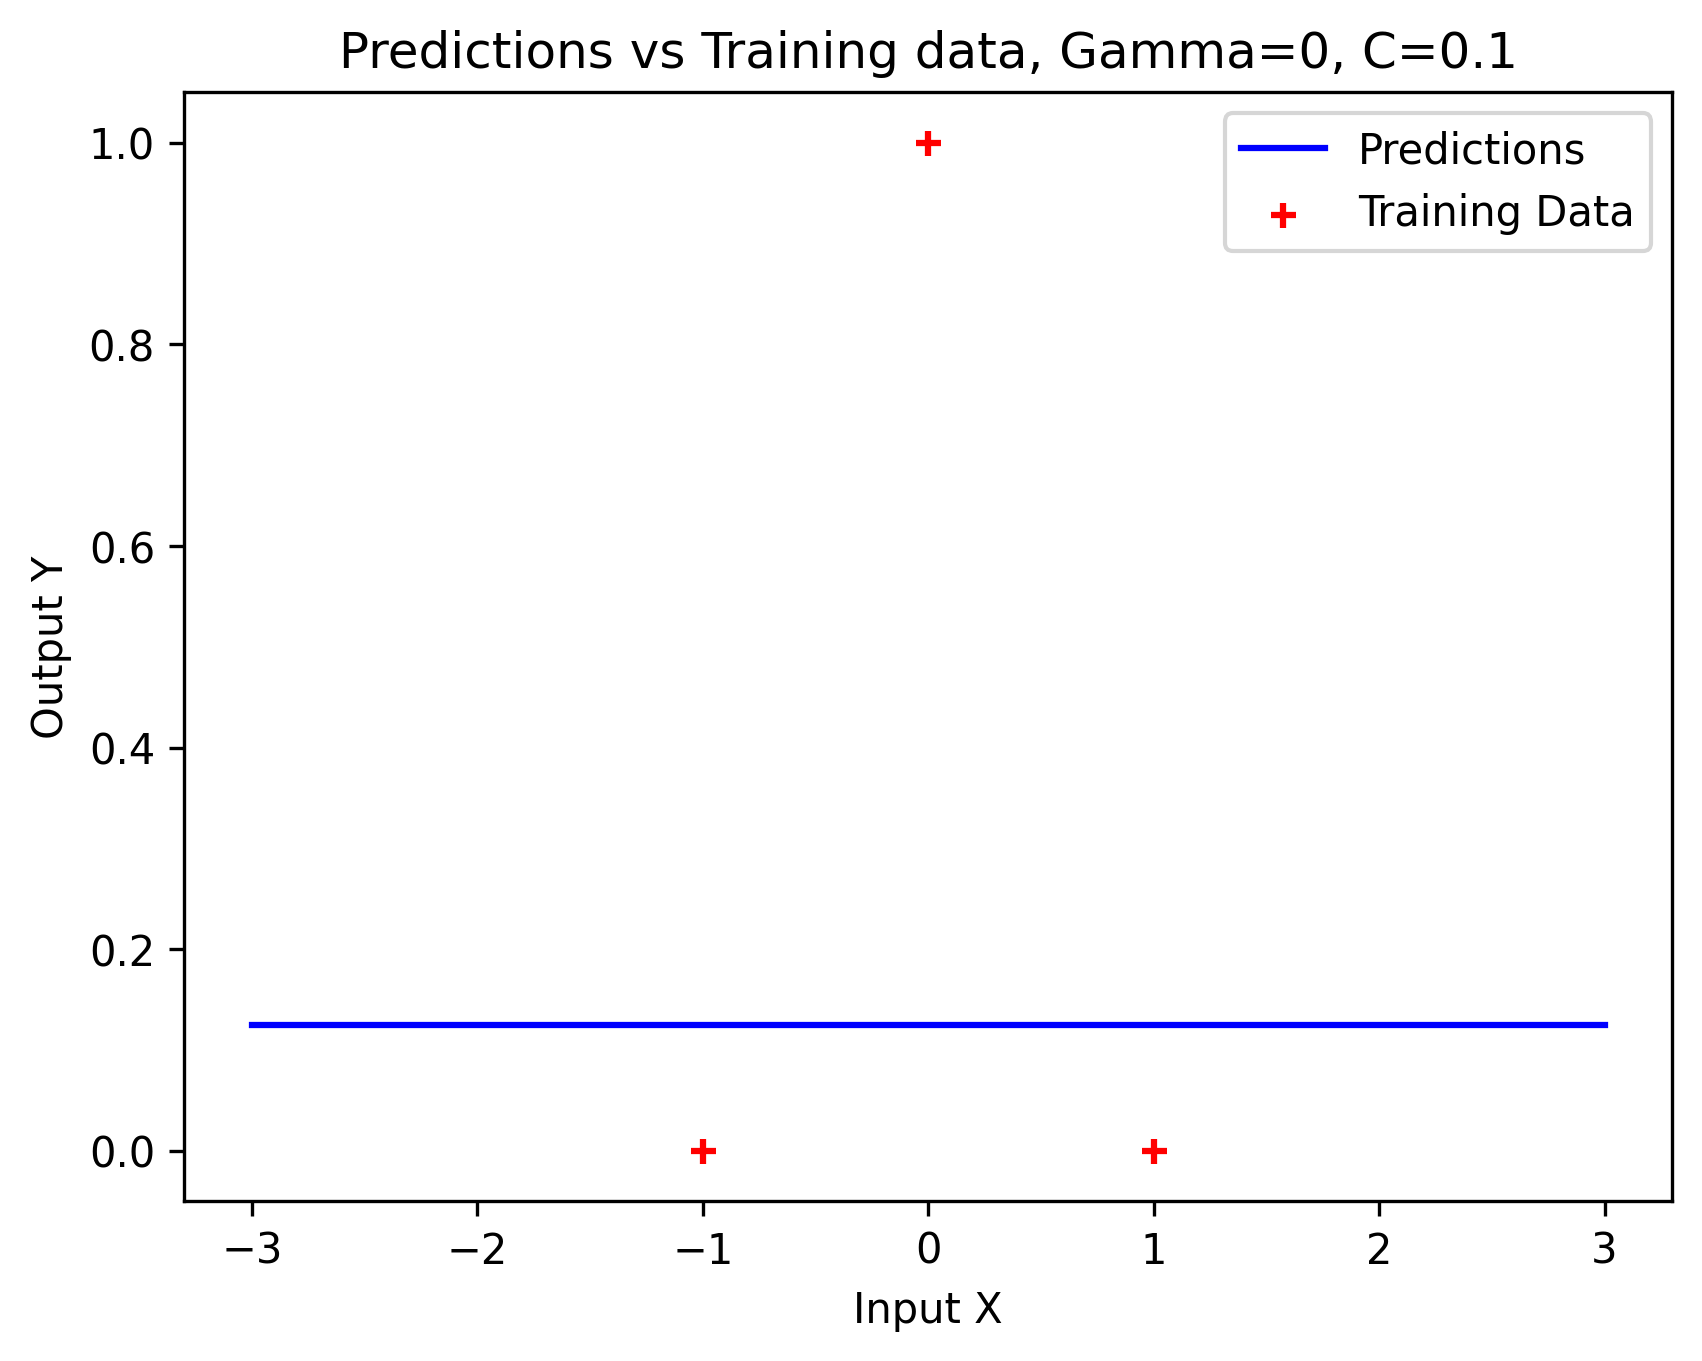
\includegraphics[width=8cm]{kr00.png}}}
\qquad
\subfloat[Gamma = 1, C = 0.1]{{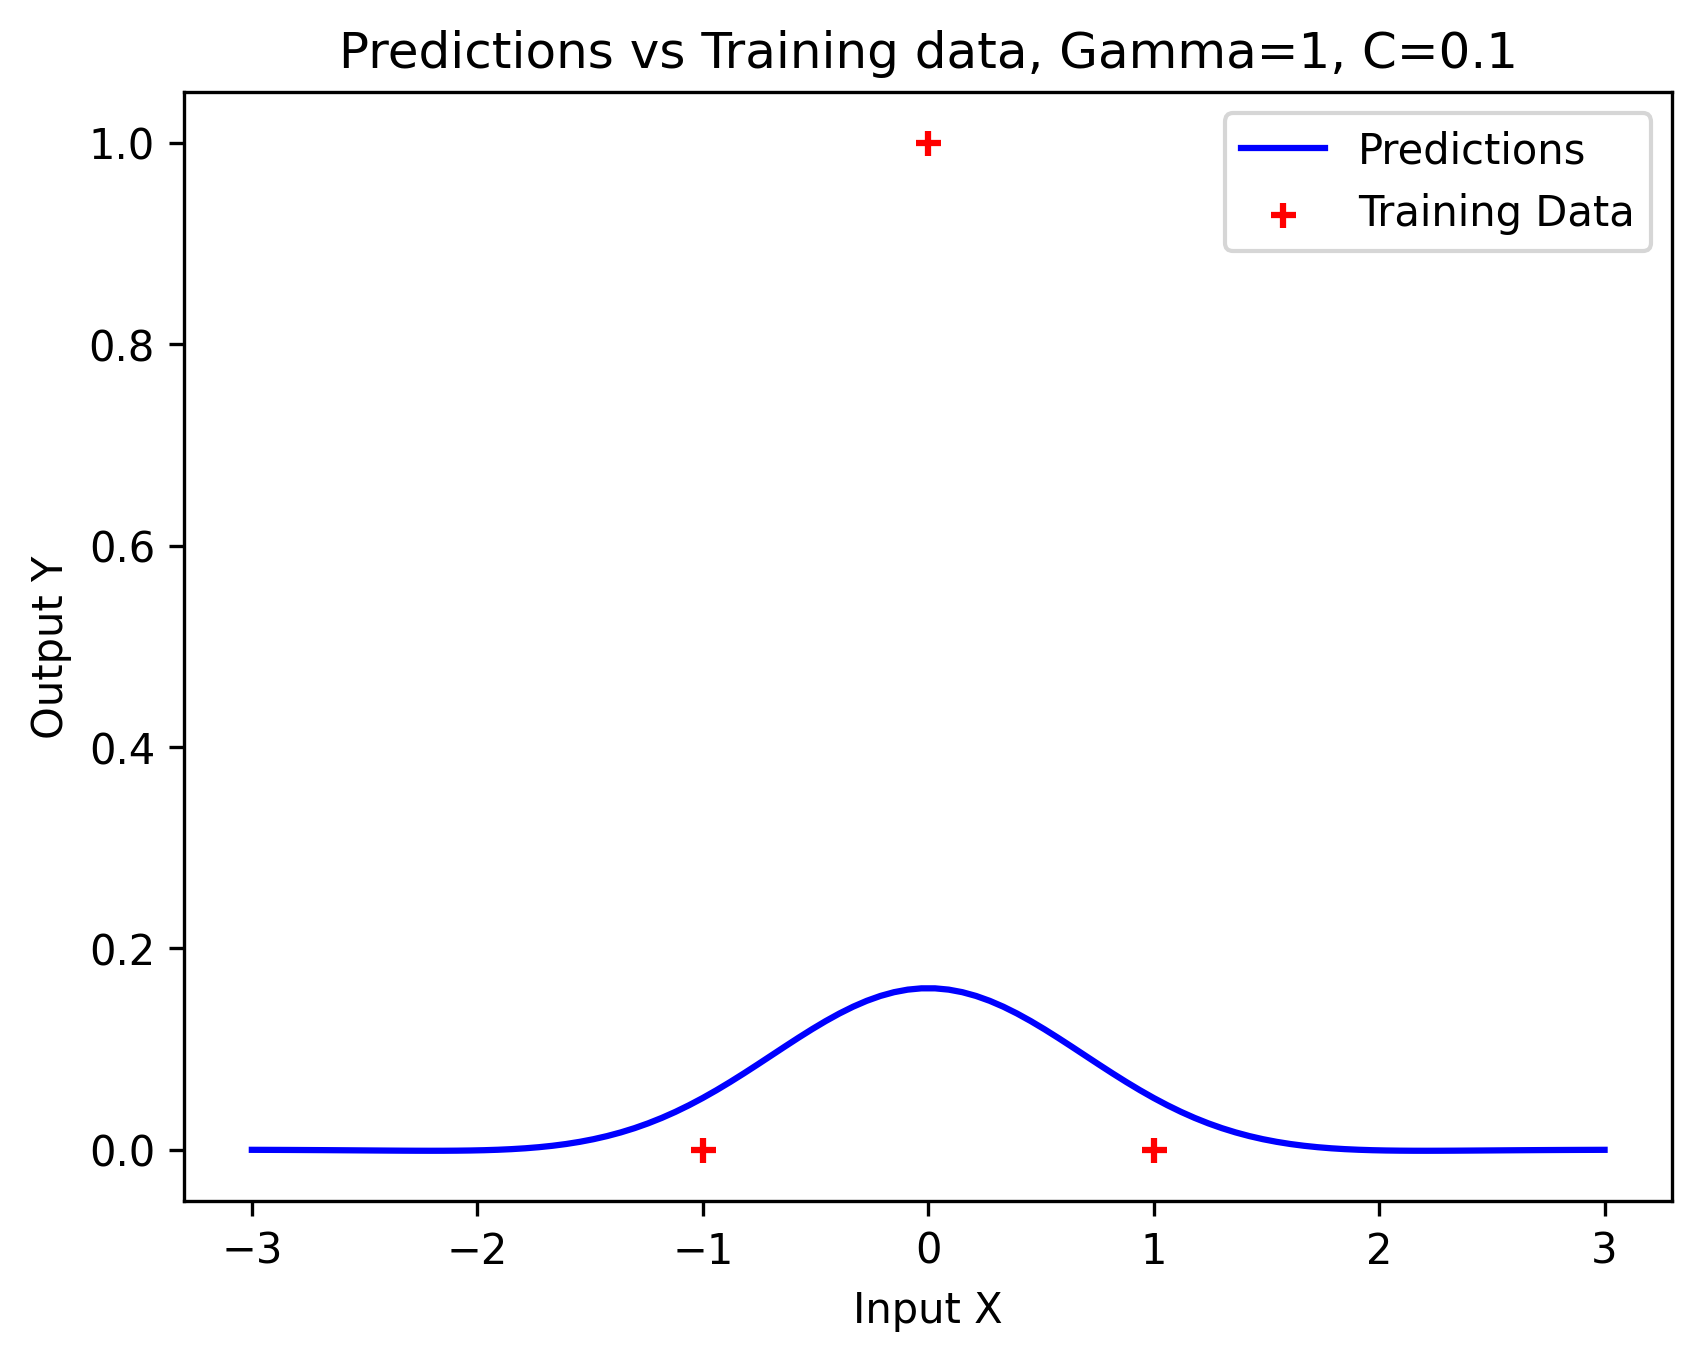
\includegraphics[width=8cm]{kr01.png}}}
\qquad
\subfloat[Gamma = 5, C= 0.1]{{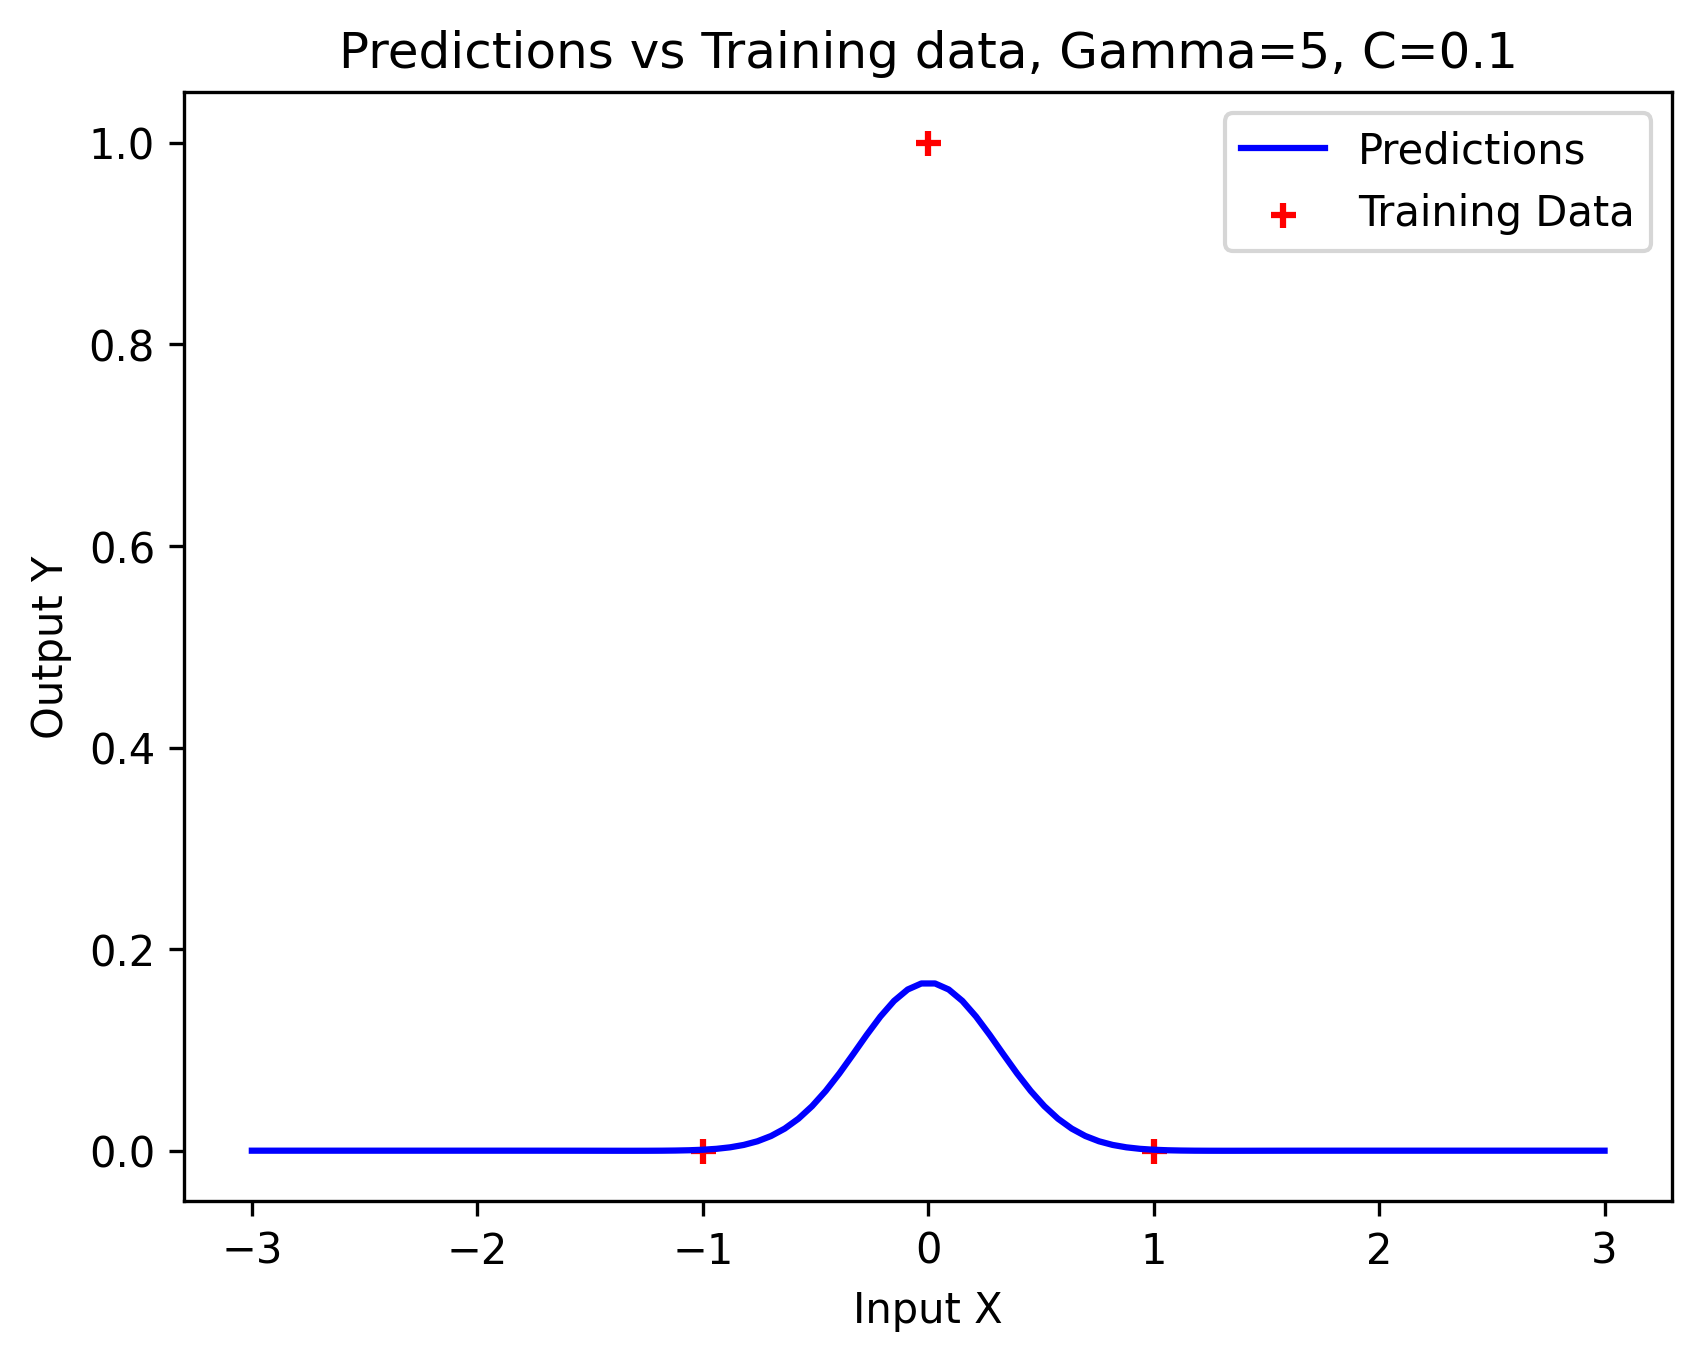
\includegraphics[width=8cm]{kr02.png}}}
\qquad
\subfloat[Gamma = 10, C= 0.1]{{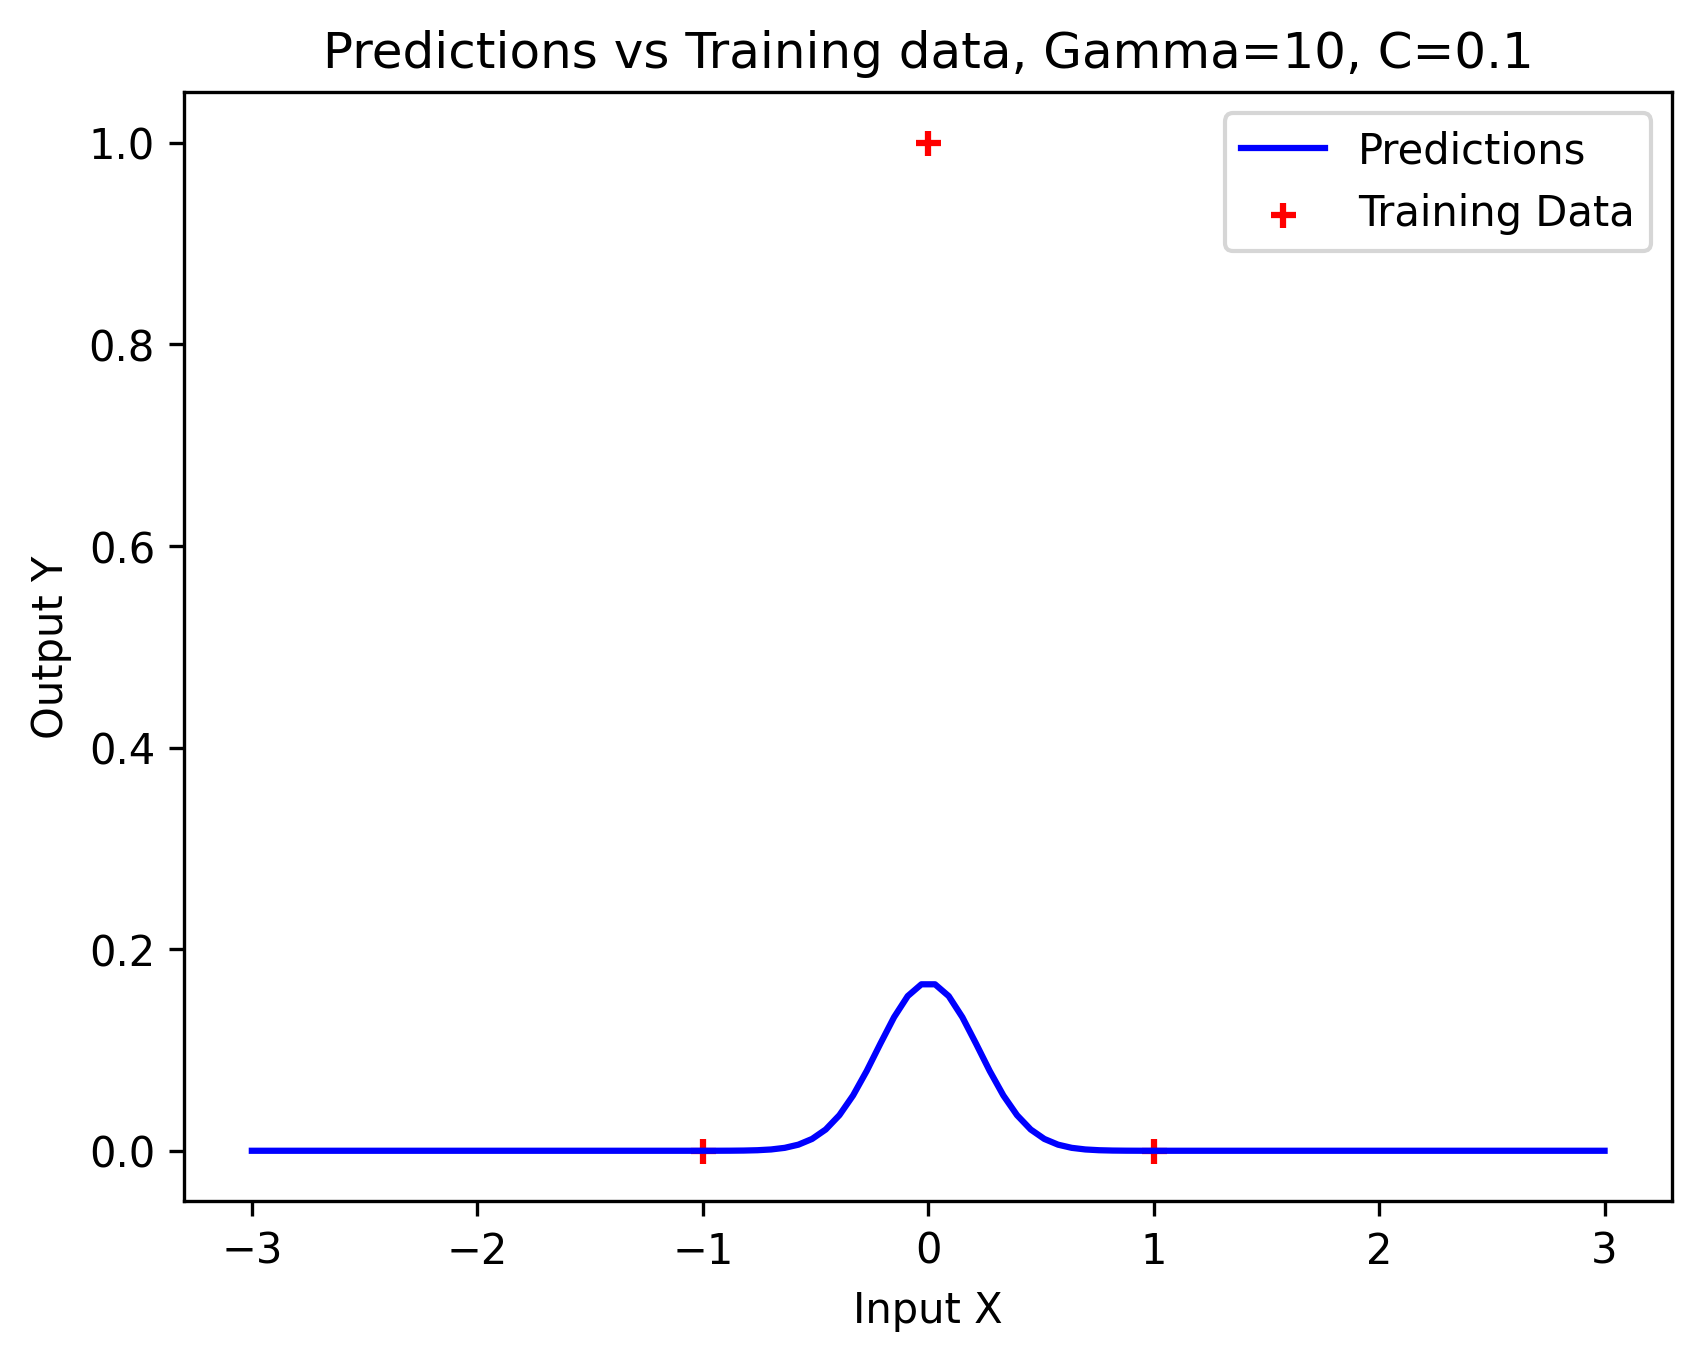
\includegraphics[width=8cm]{kr03.png}}}
\qquad
\subfloat[Gamma = 25, C= 0.1]{{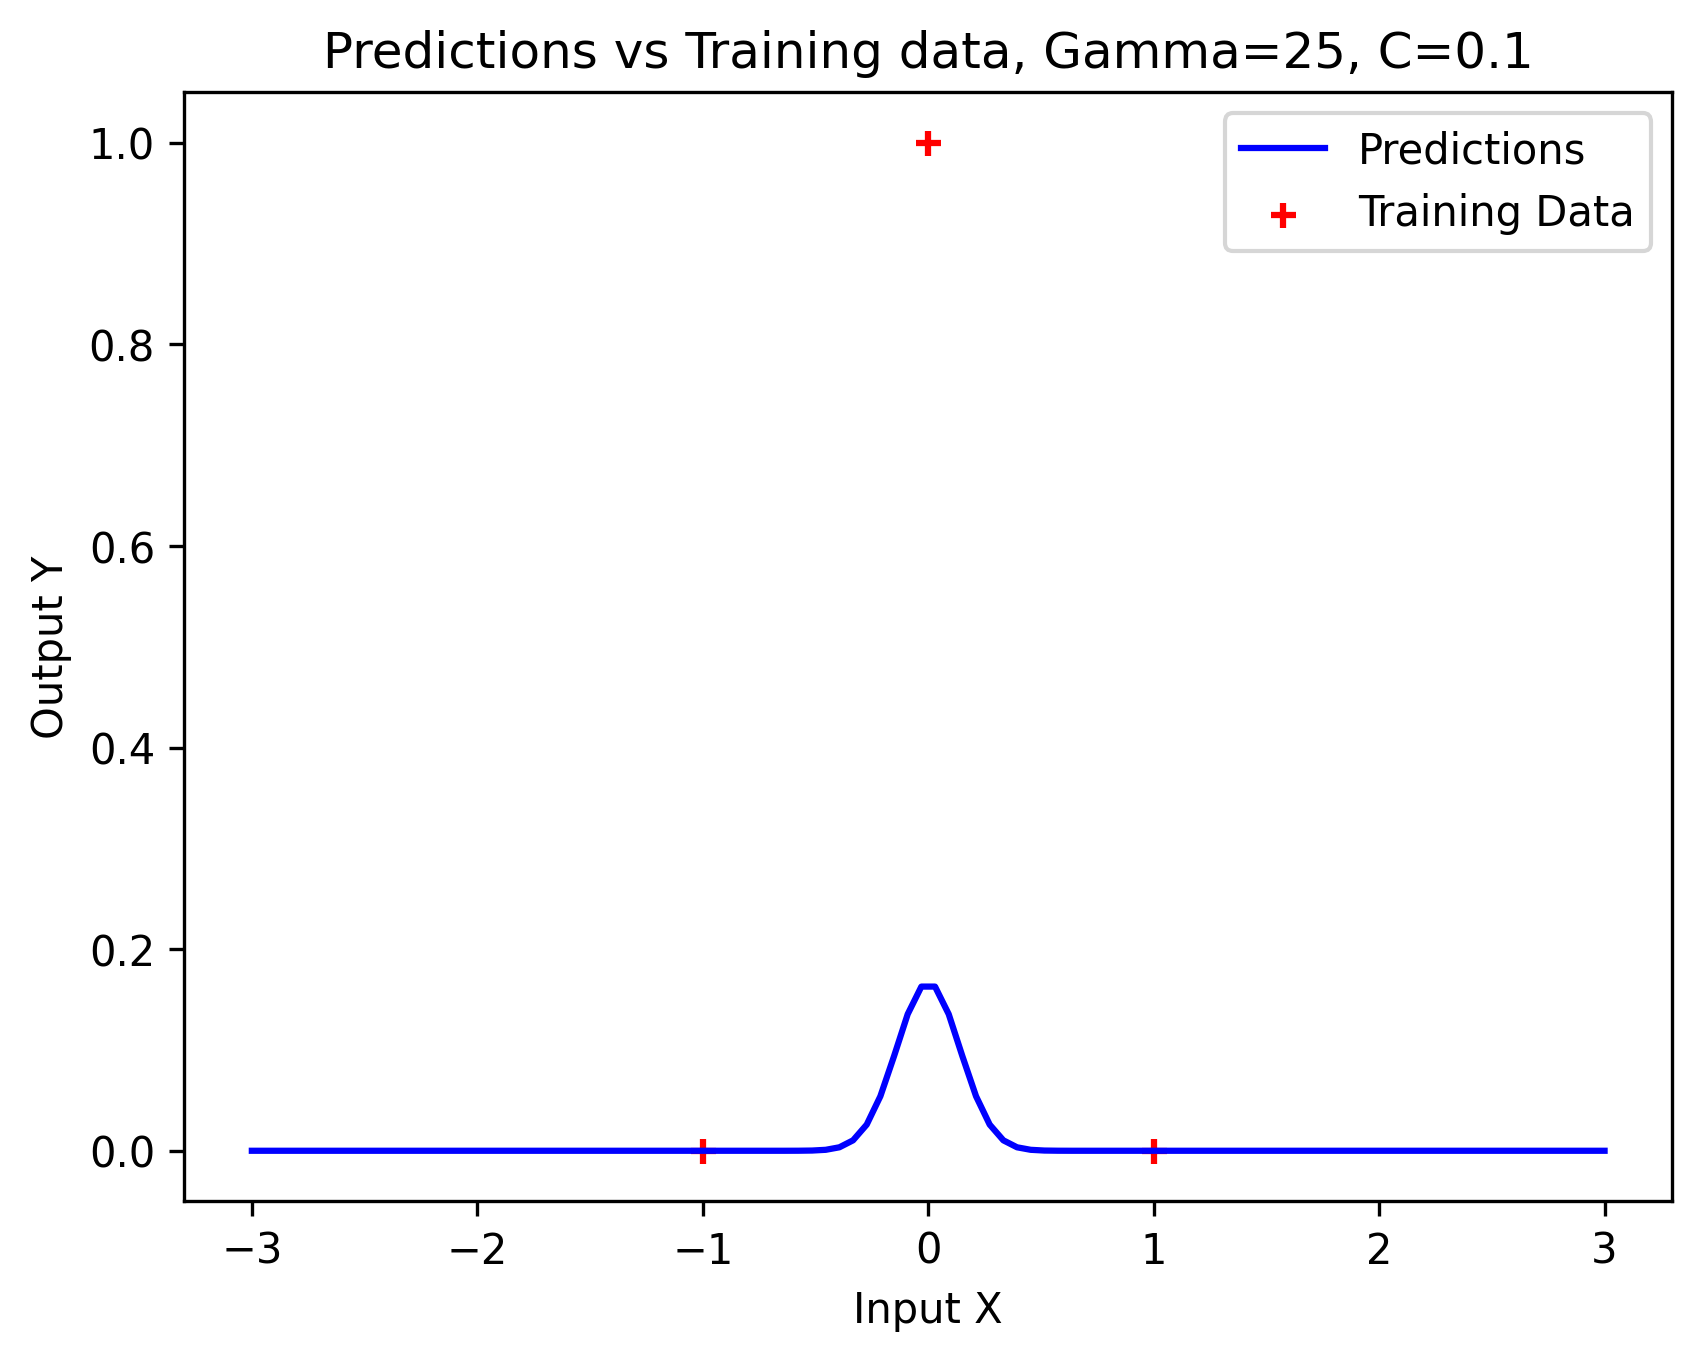
\includegraphics[width=8cm]{kr04.png}}}
\end{figure}
\(\theta_0 = -0.025, \theta_1= 0.175 , \theta_2= -0.025\)\\
\(\theta_0= -0.0103, \theta_1= 0.1679 , \theta_2 =-0.0103\)\\
\(\theta_0 =-0.0002, \theta_1= 0.1667 , \theta_2 =-0.0002\)\\
\(\theta_0 =-0.0, \theta_1 =0.1667 , \theta_2 =-0.0\)\\
\(\theta_0 =-0.0, \theta_1= 0.1667 , \theta_2 =-0.0\)\\

\begin{figure}[h]
\centering
\subfloat[Gamma = 0, C = 1]{{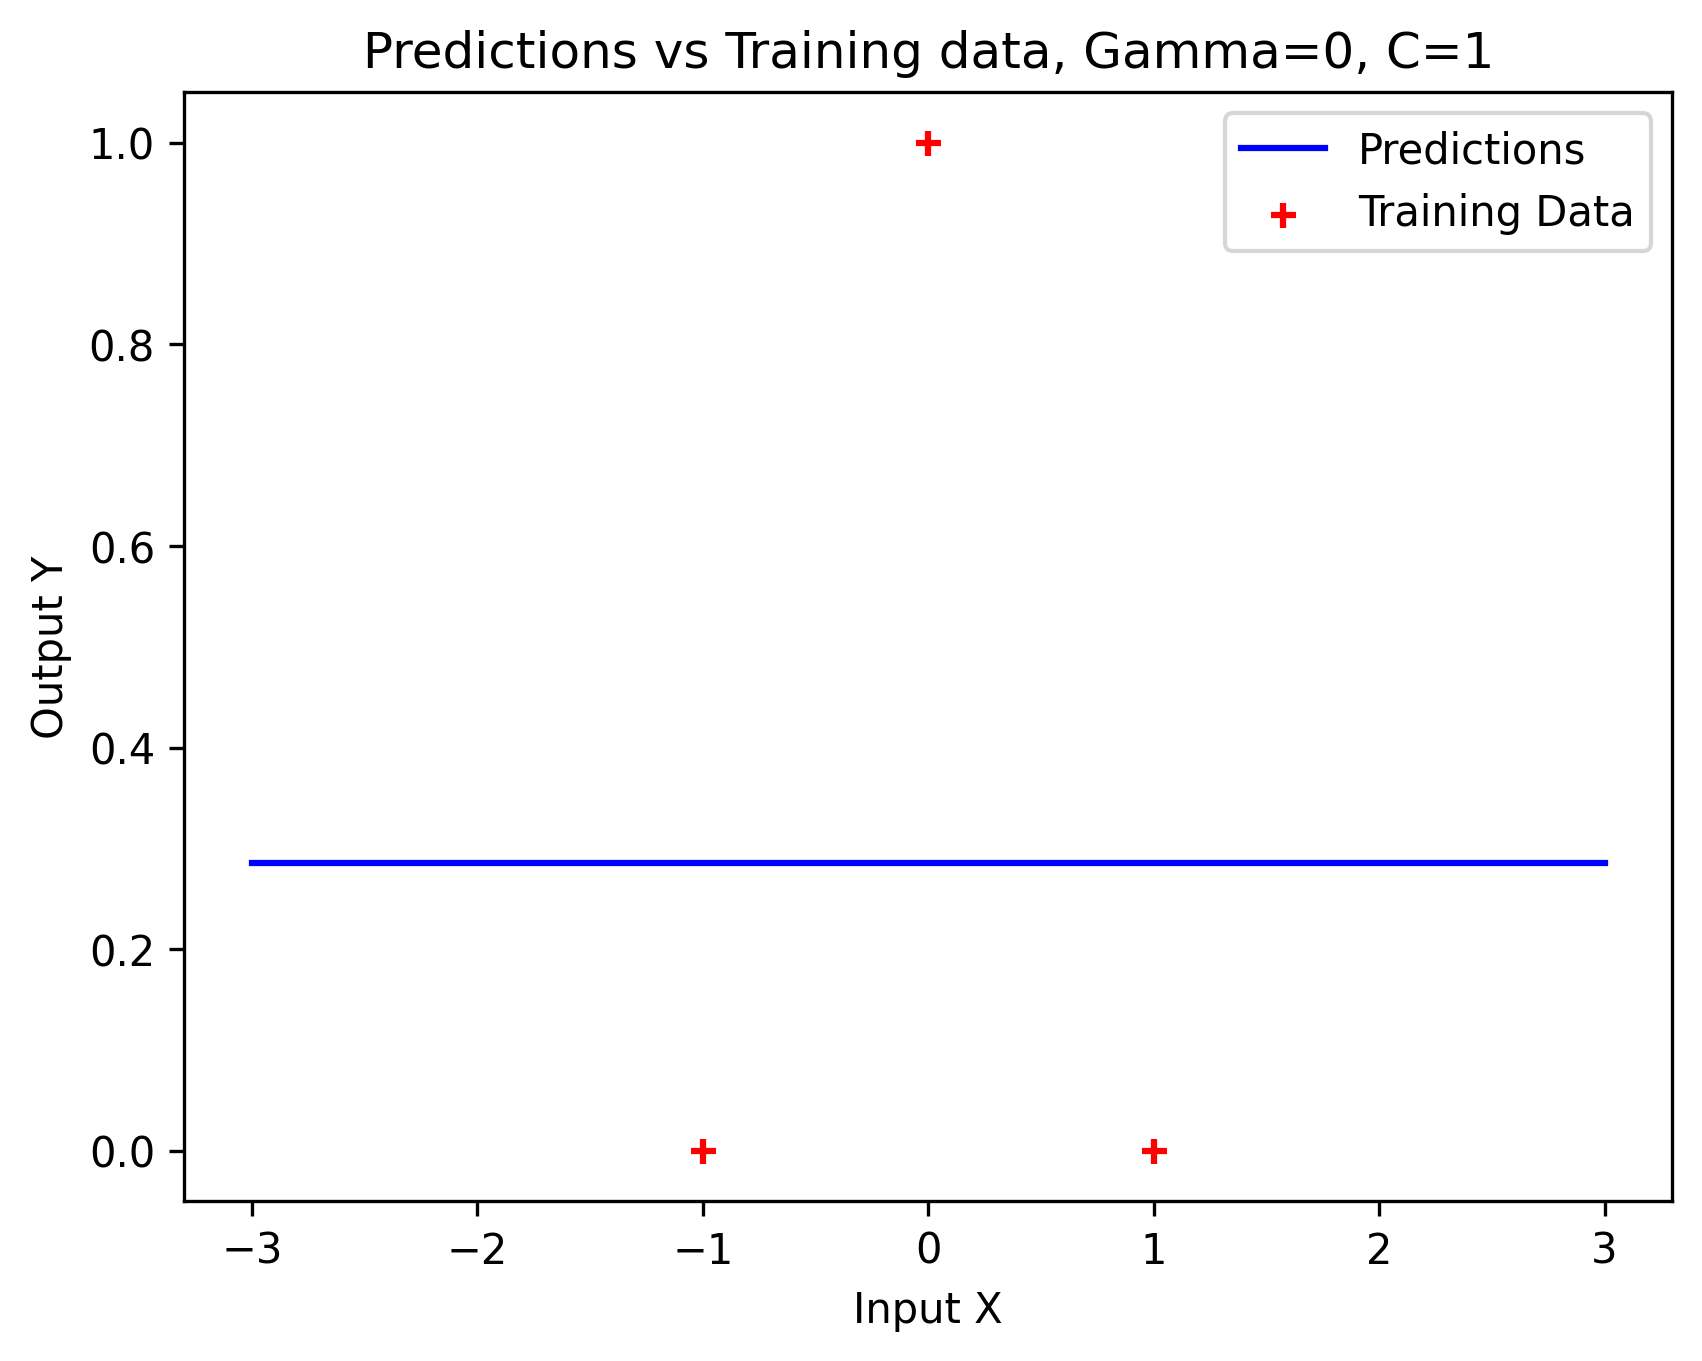
\includegraphics[width=8cm]{kr10.png}}}
\qquad
\subfloat[Gamma = 1, C = 1]{{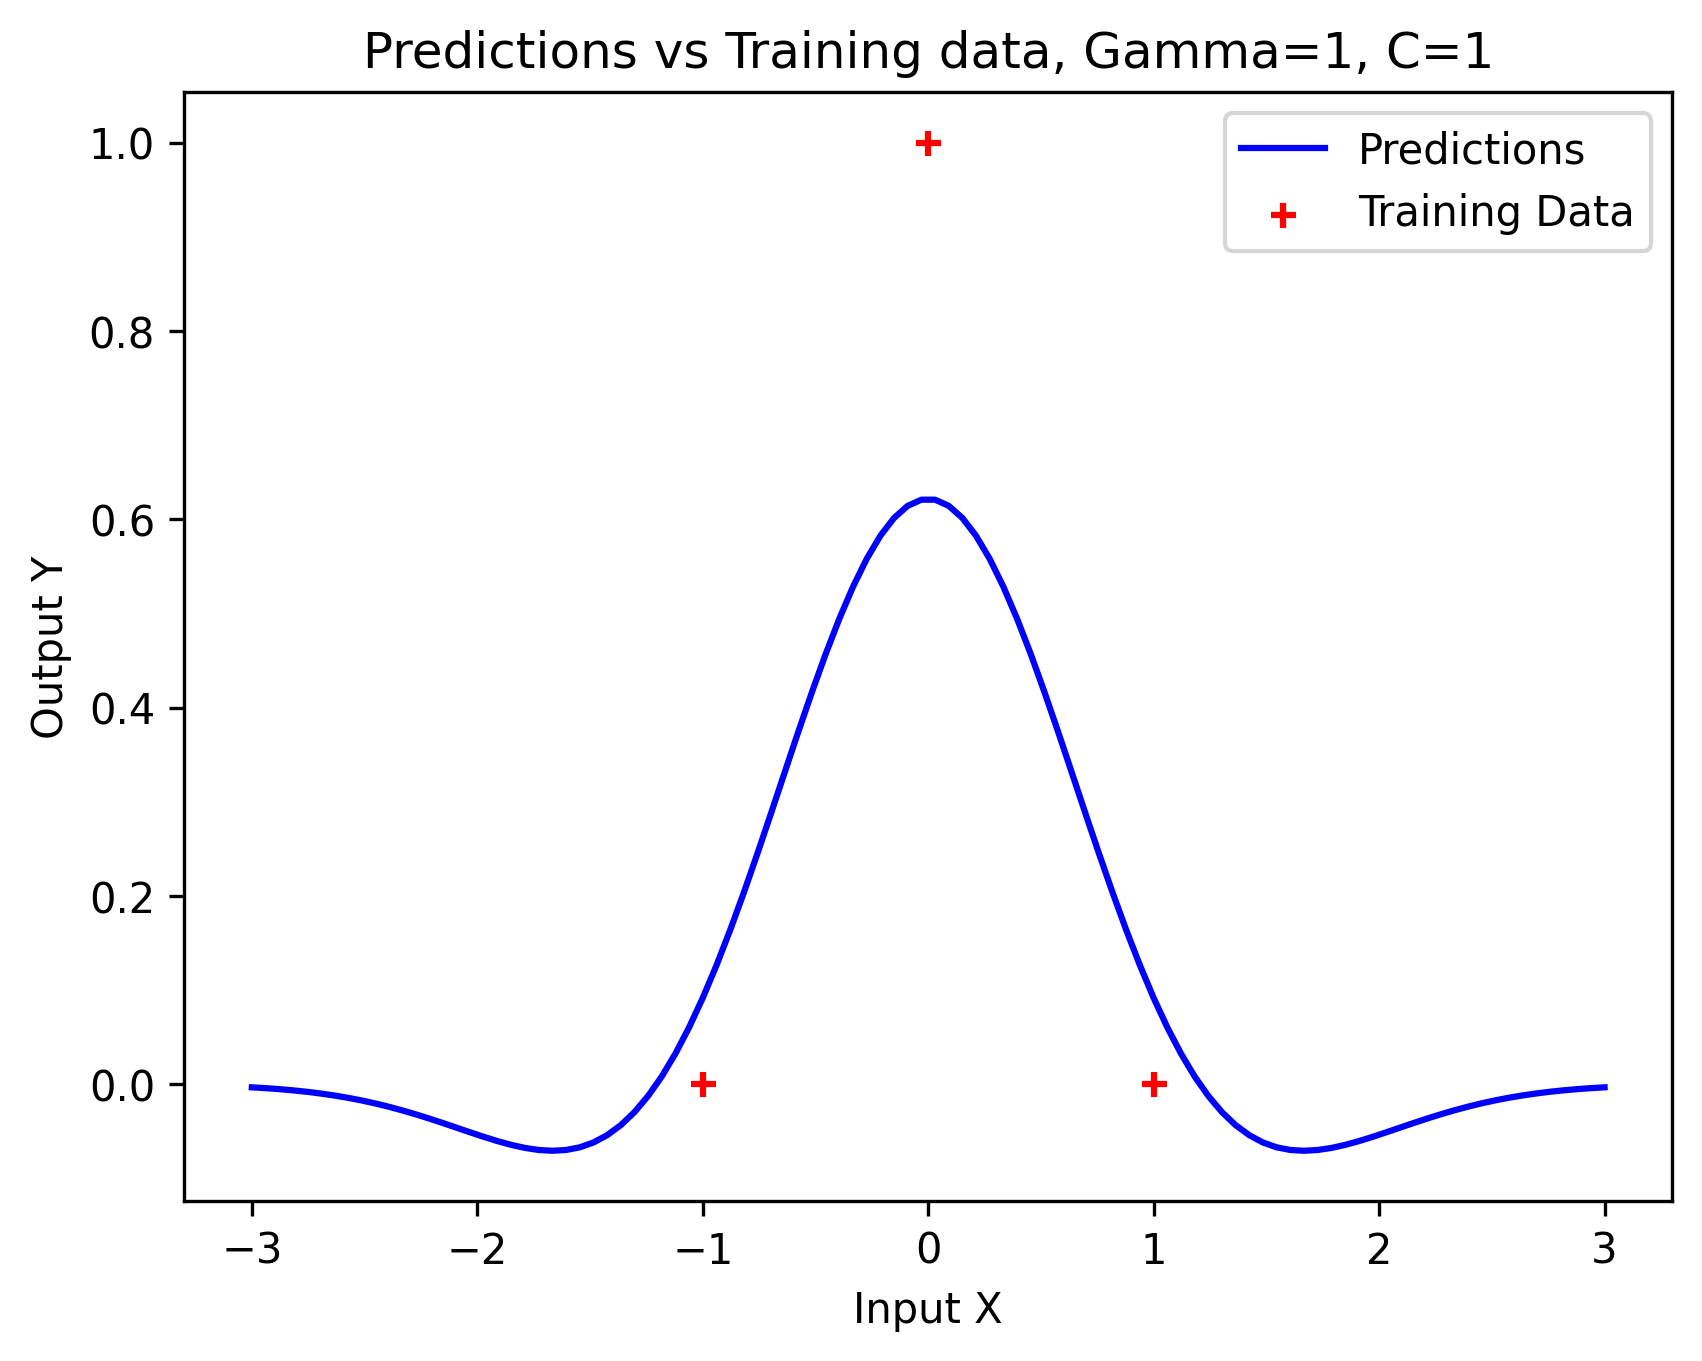
\includegraphics[width=8cm]{kr11.png}}}
\qquad
\subfloat[Gamma = 5, C= 1]{{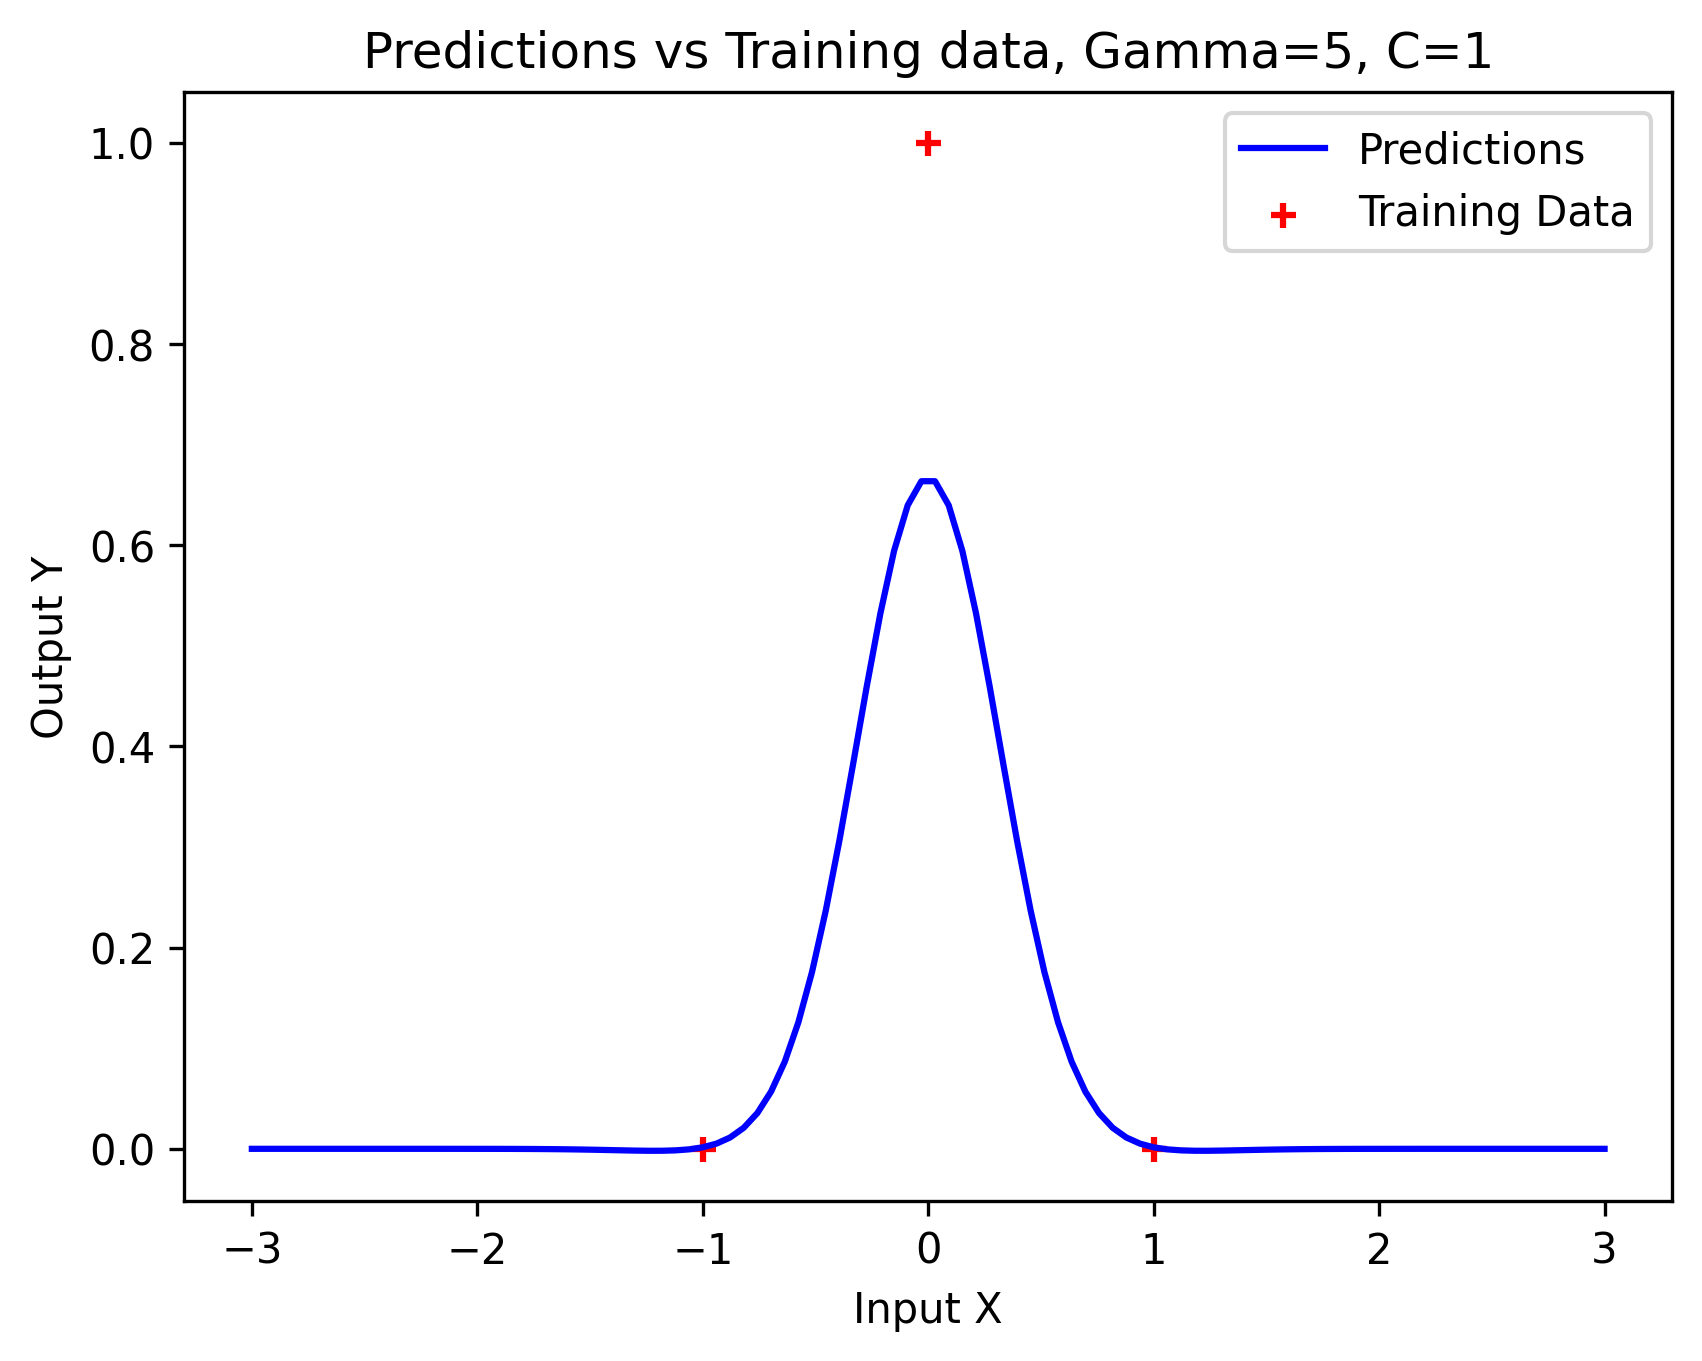
\includegraphics[width=8cm]{kr12.png}}}
\qquad
\subfloat[Gamma = 10, C= 1]{{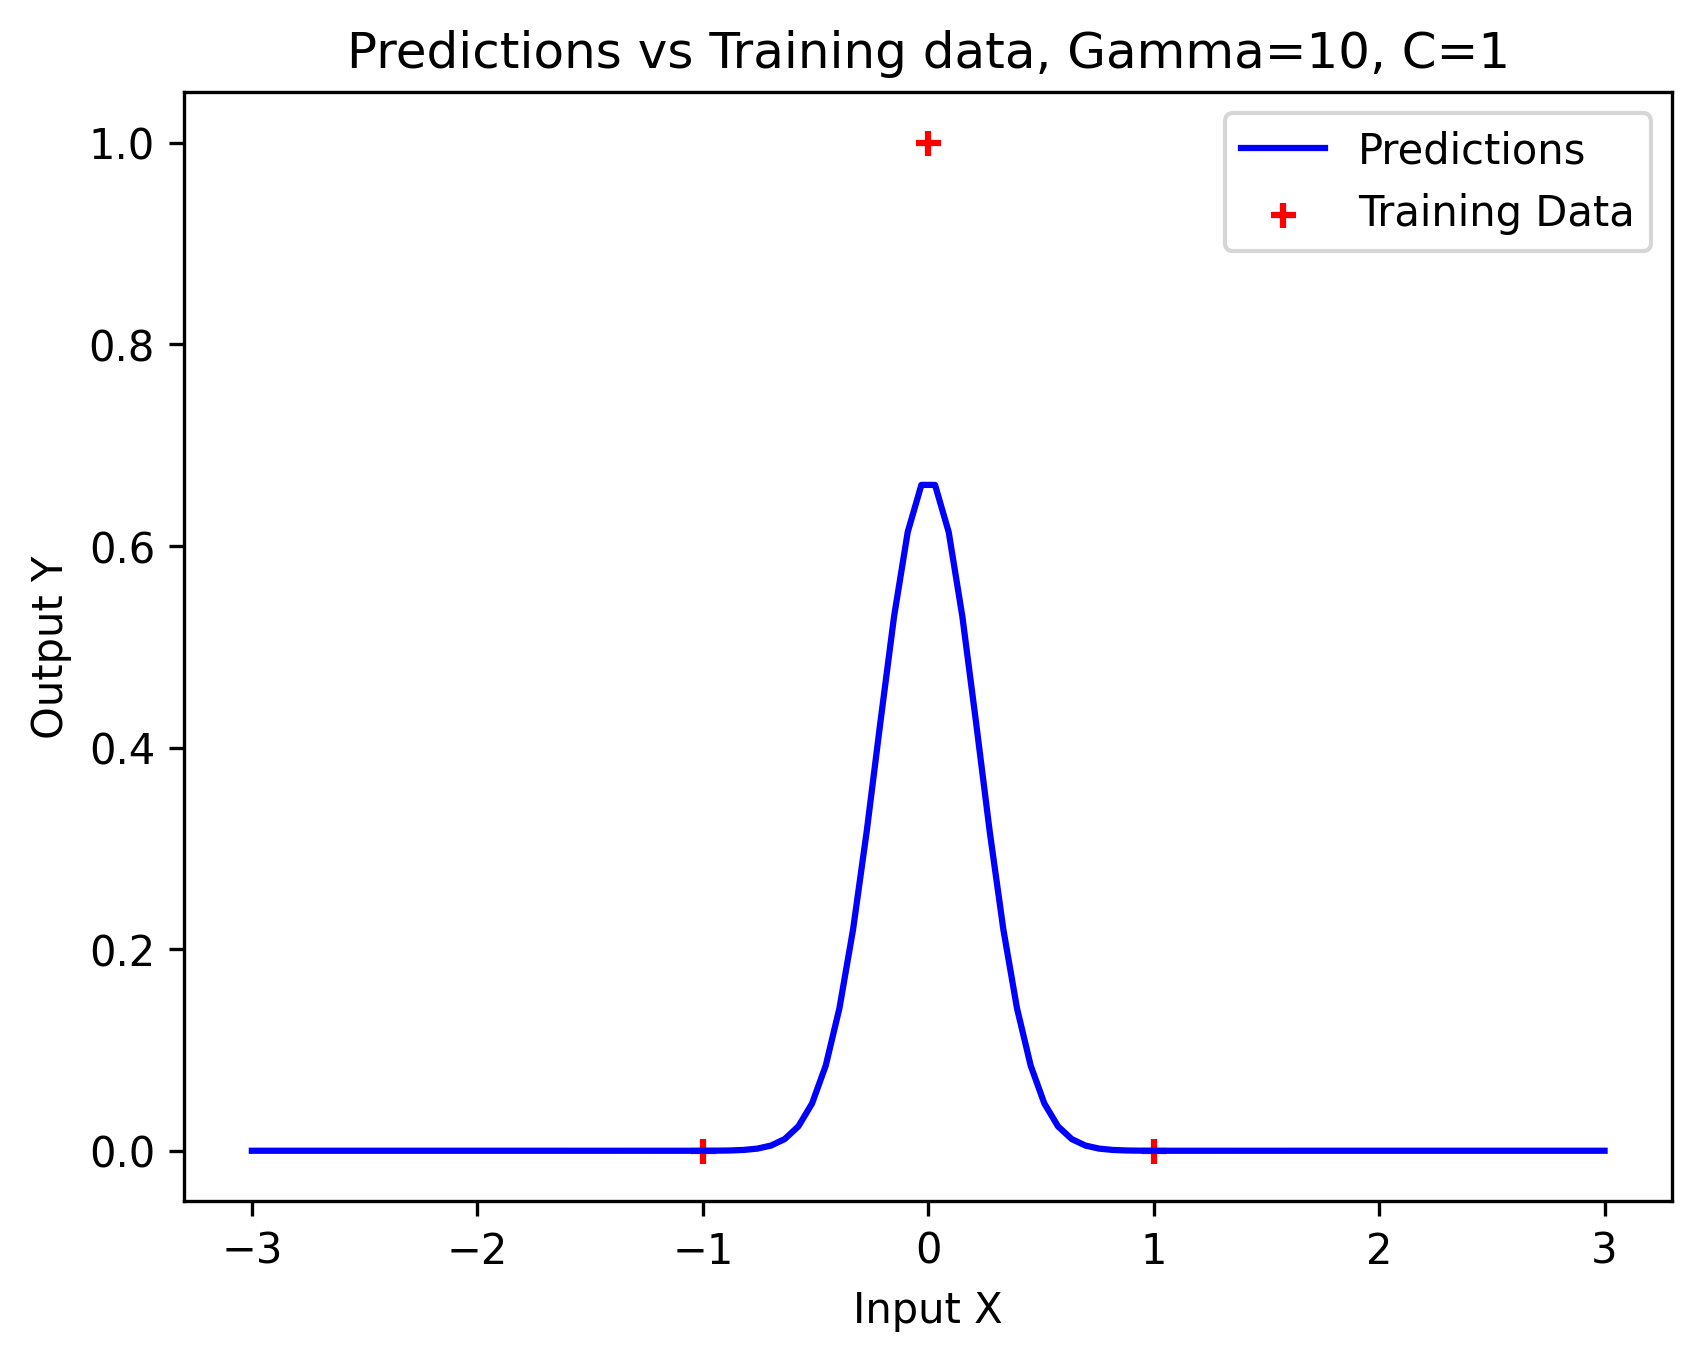
\includegraphics[width=8cm]{kr13.png}}}
\qquad
\subfloat[Gamma = 25, C= 1]{{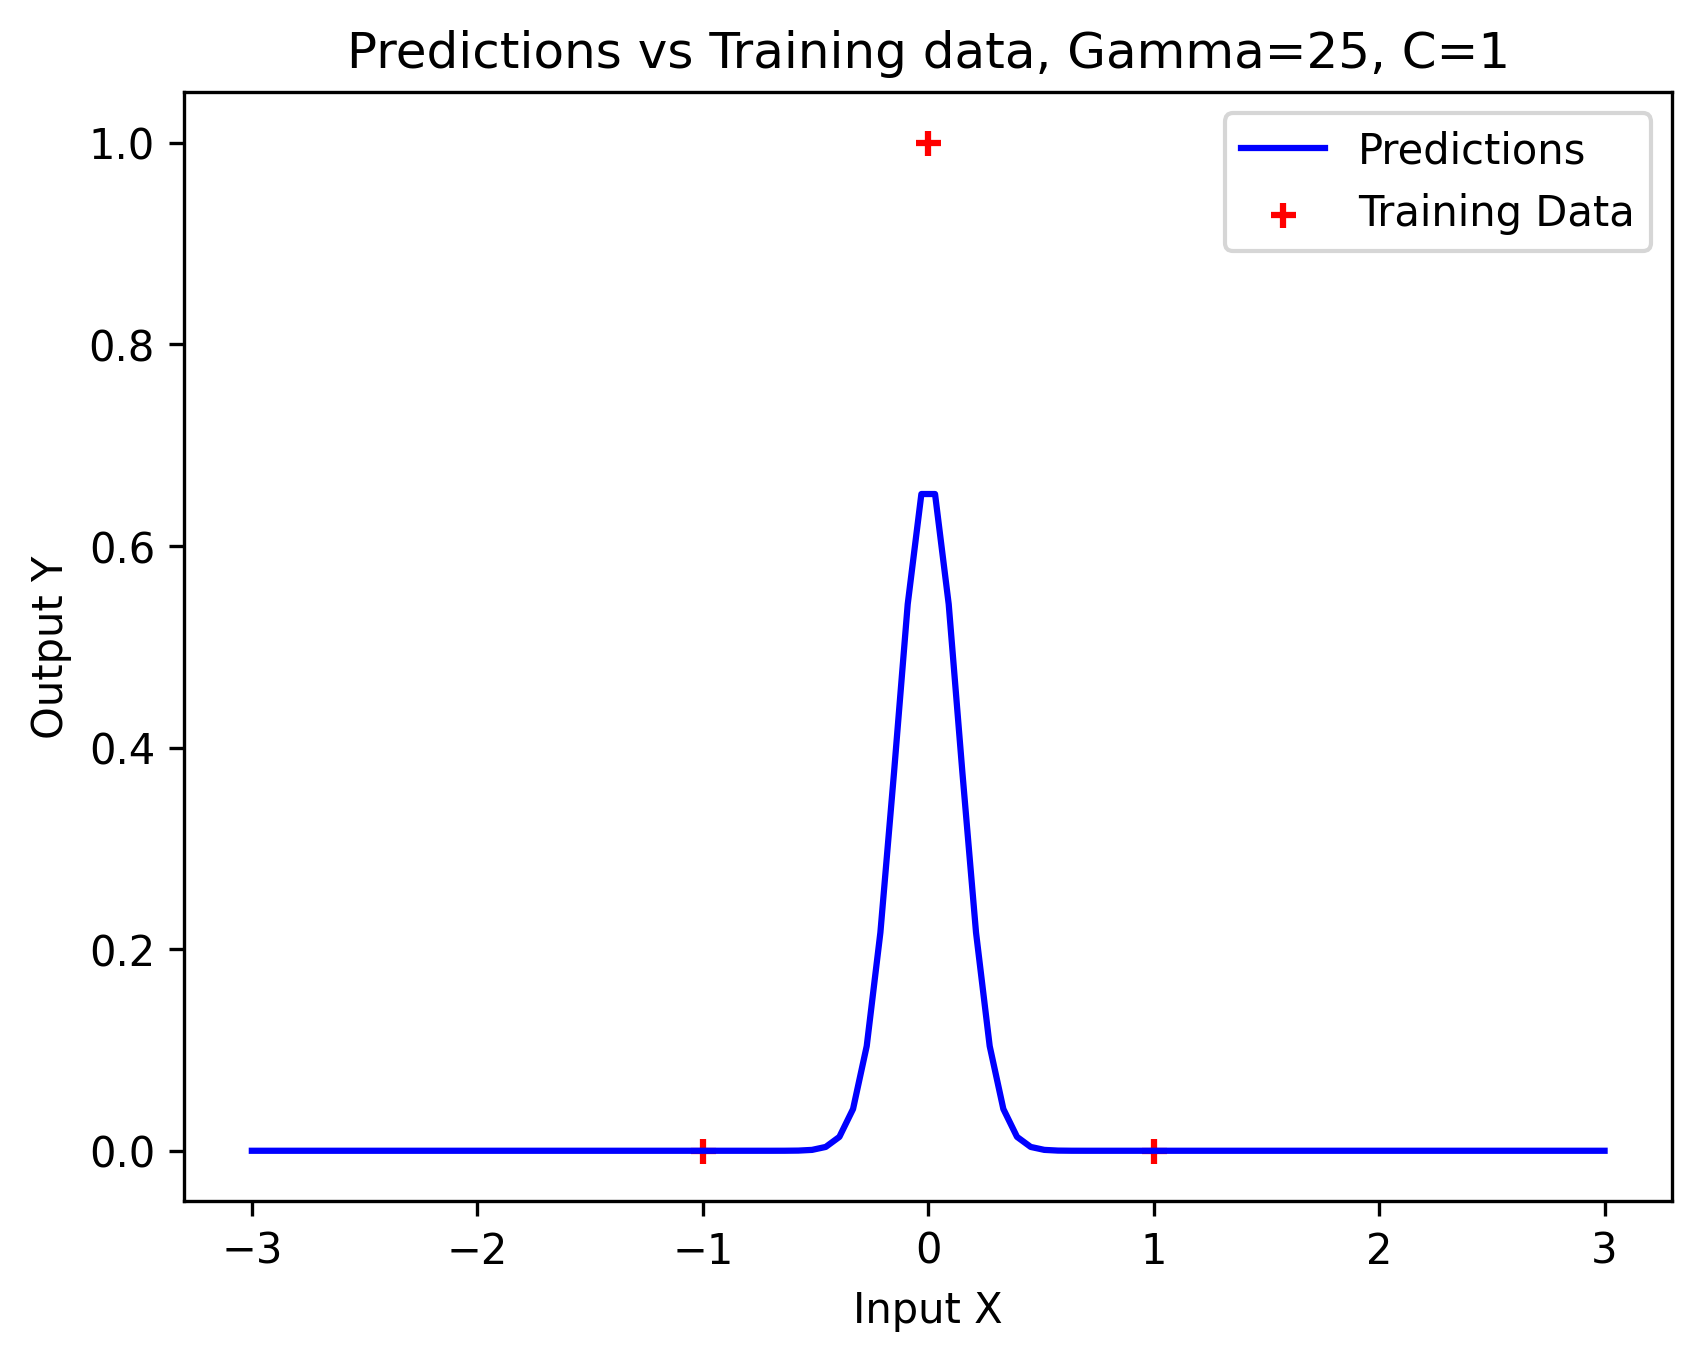
\includegraphics[width=8cm]{kr14.png}}}
\end{figure}
\(\theta_0= -0.5714, \theta_1= 1.4286 , \theta_2 =-0.5714\)\\
\(\theta_0 =-0.1833, \theta_1= 0.7566 , \theta_2 =-0.1833\)\\
\(\theta_0 =-0.003, \theta_1= 0.6667 , \theta_2 =-0.003\)\\
\(\theta_0 =-0.0, \theta_1= 0.6667 , \theta_2= -0.0\)\\
\(\theta_0 =-0.0, \theta_1 =0.6667 , \theta_2 =-0.0\)\\

\begin{figure}[h]
\centering
\subfloat[Gamma = 0, C = 10]{{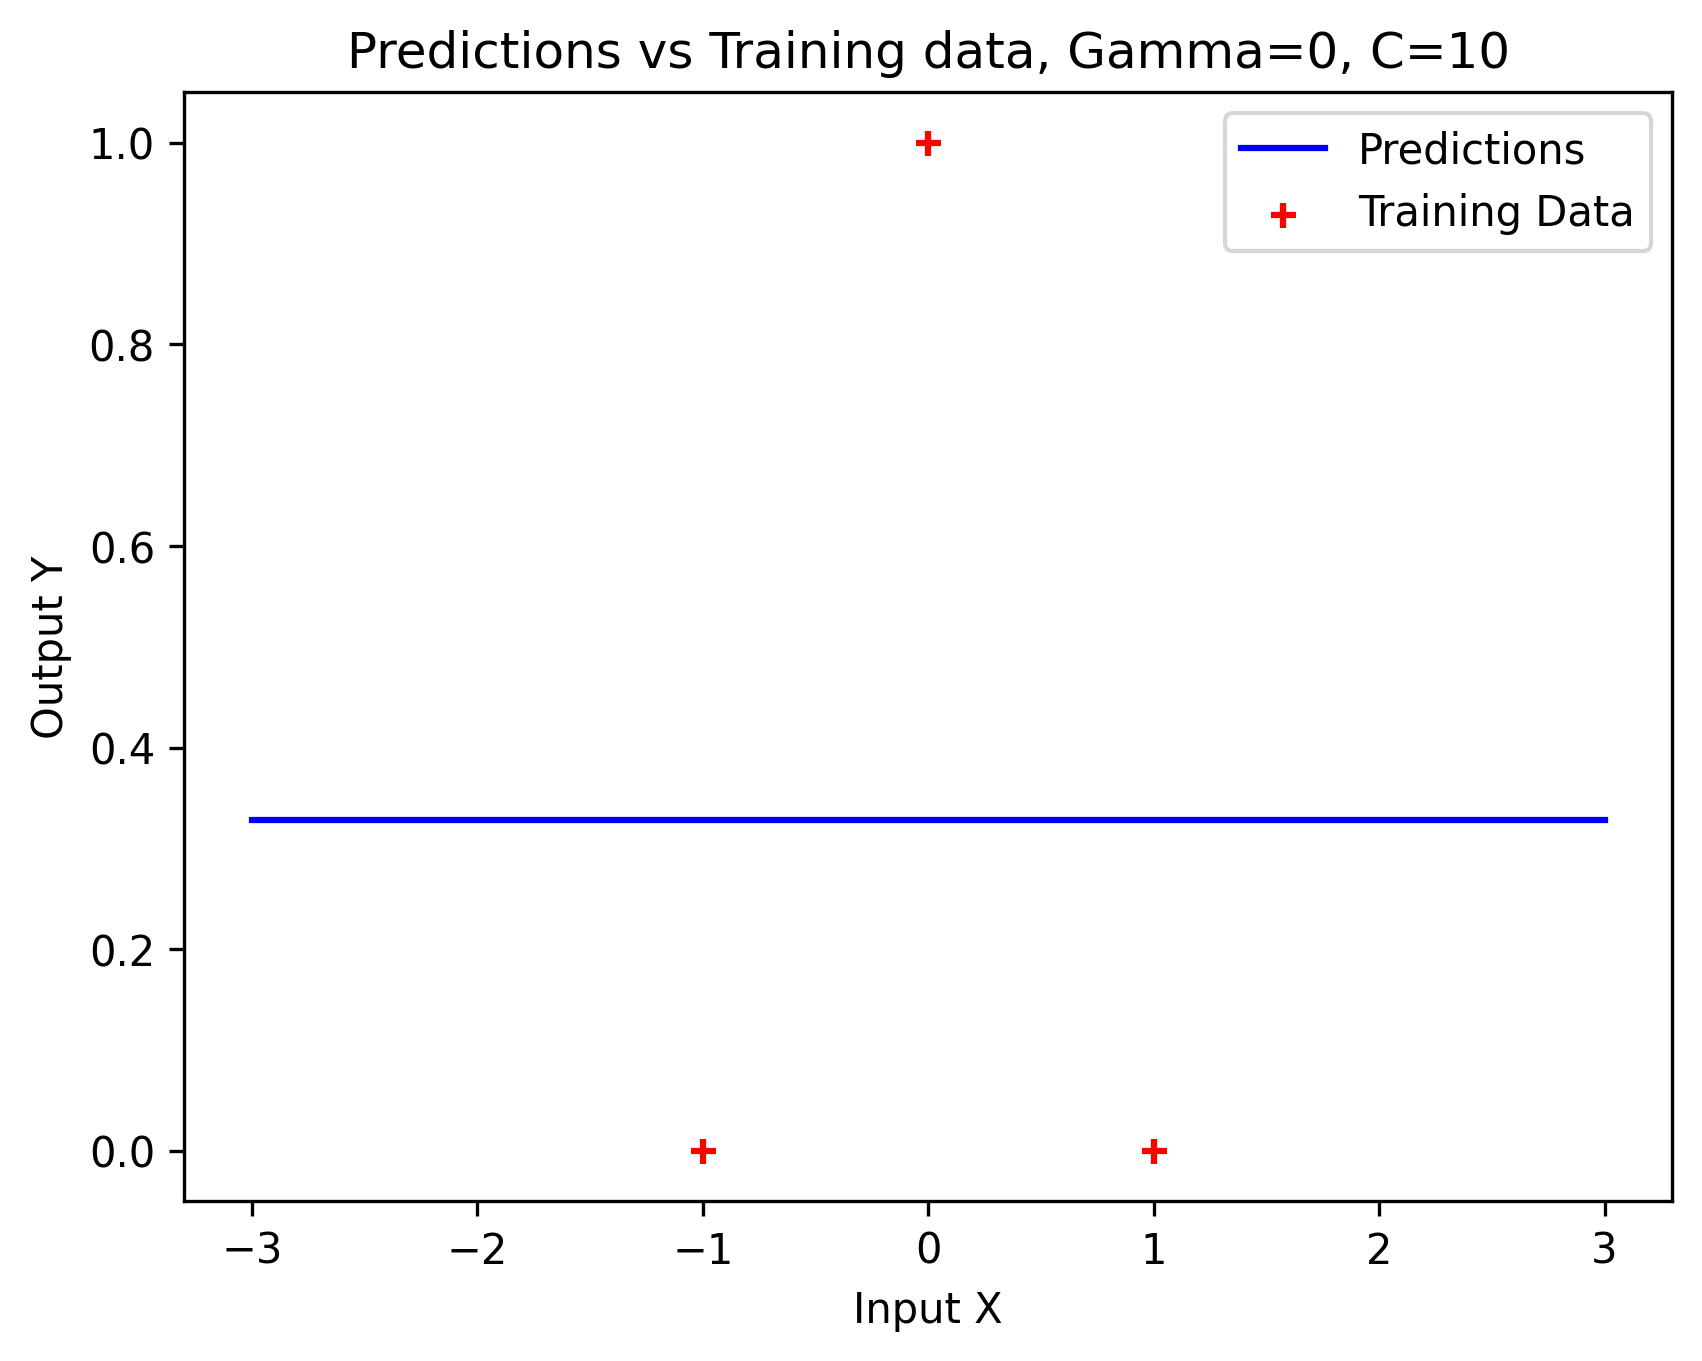
\includegraphics[width=8cm]{kr20.png}}}
\qquad
\subfloat[Gamma = 1, C = 10]{{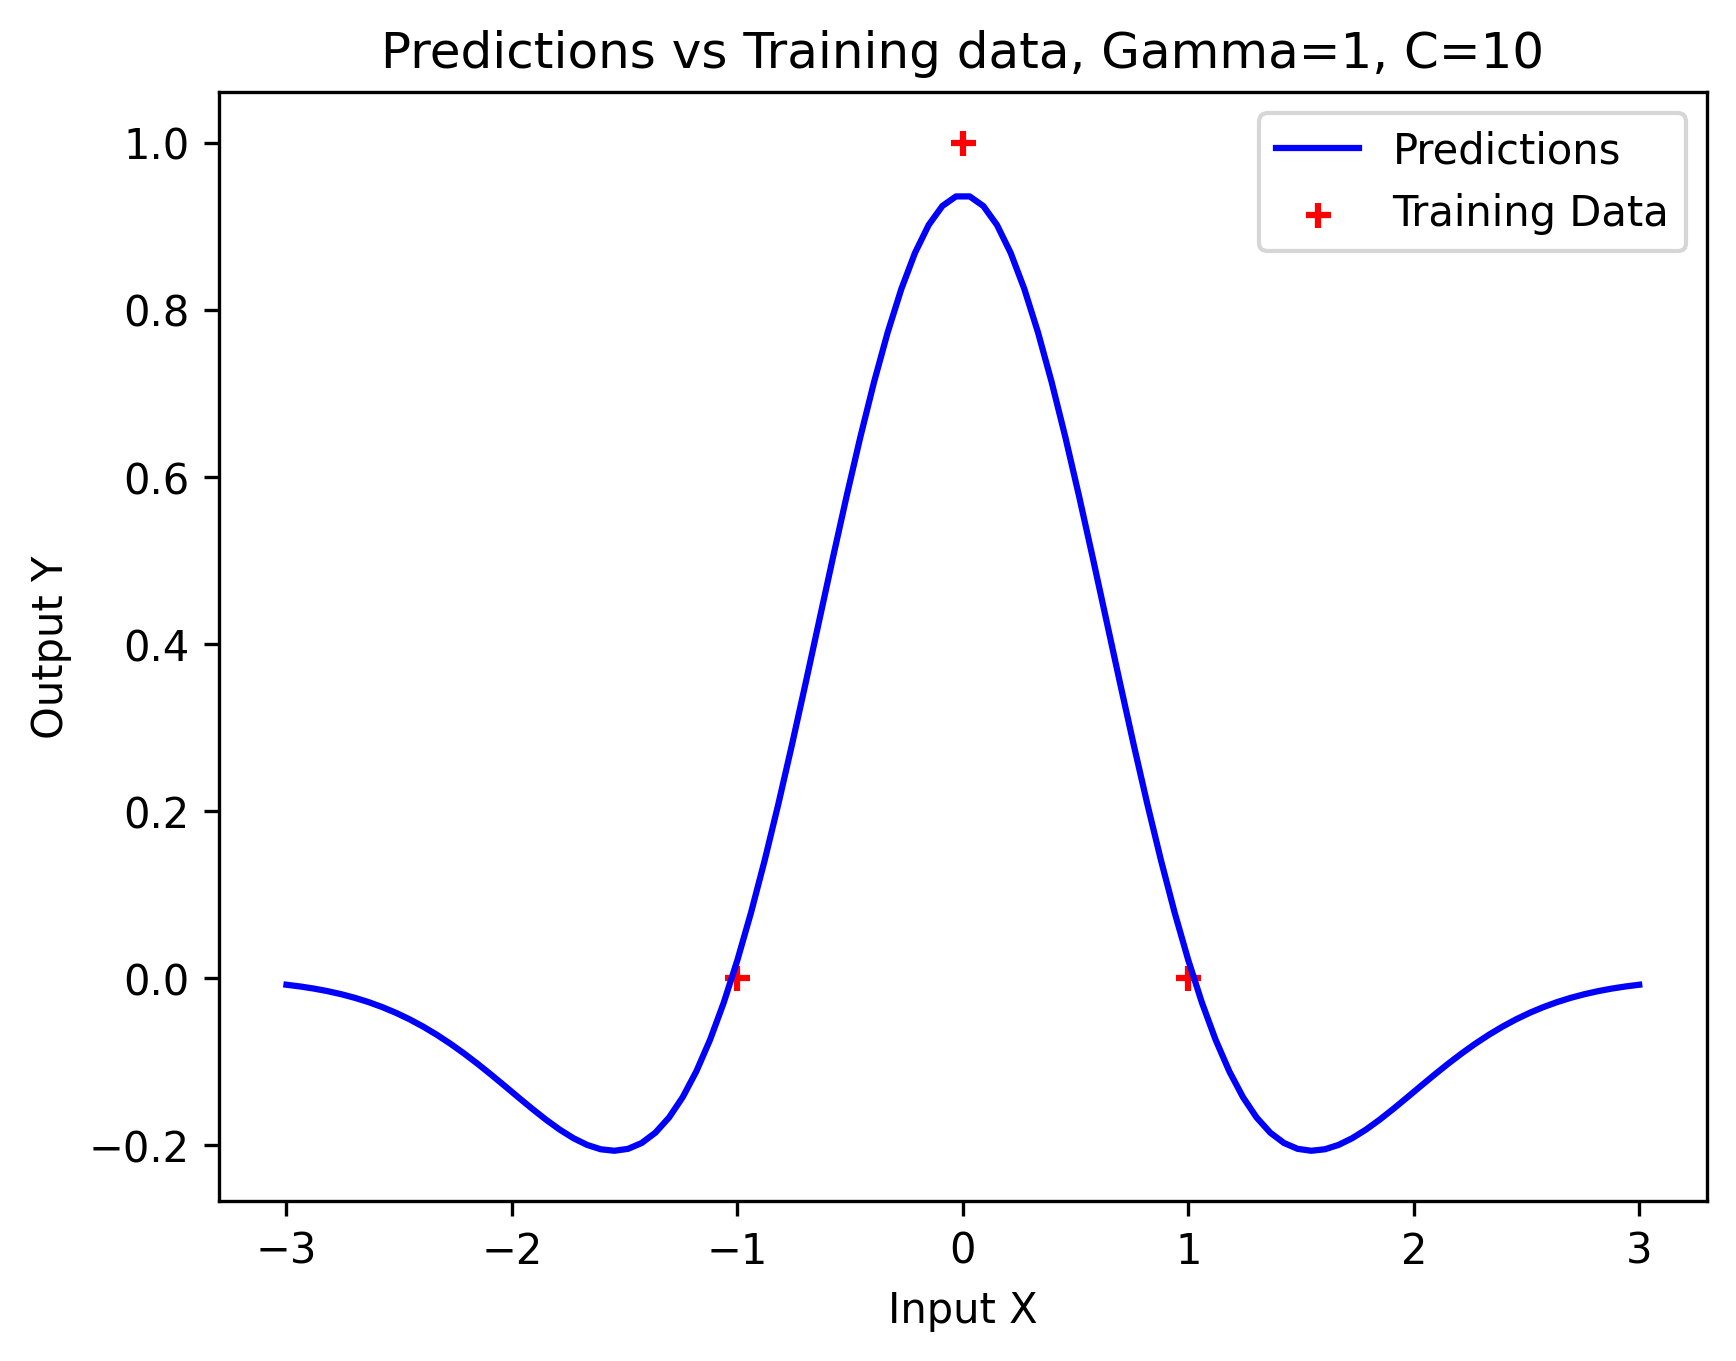
\includegraphics[width=8cm]{kr21.png}}}
\qquad
\subfloat[Gamma = 5, C= 10]{{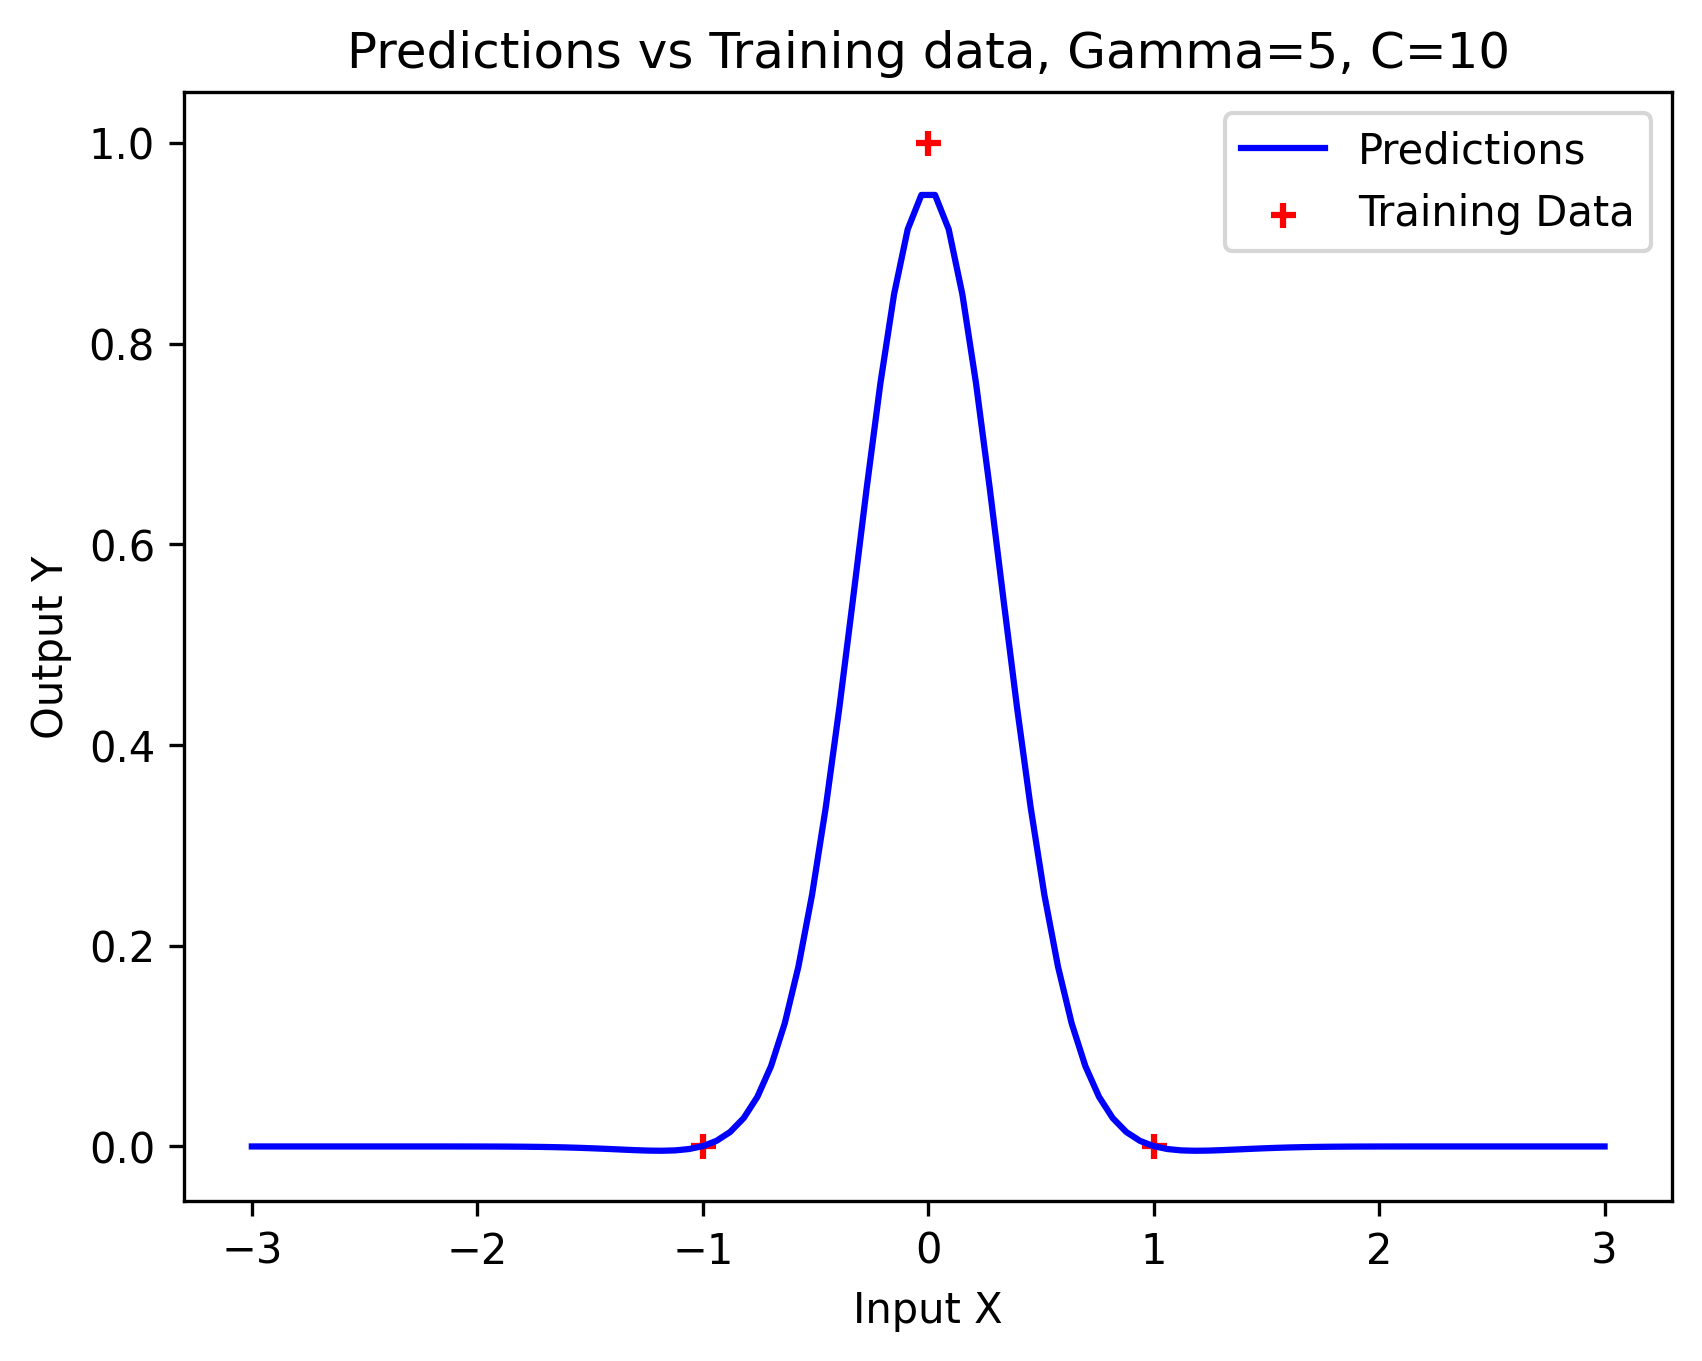
\includegraphics[width=8cm]{kr22.png}}}
\qquad
\subfloat[Gamma = 10, C= 10]{{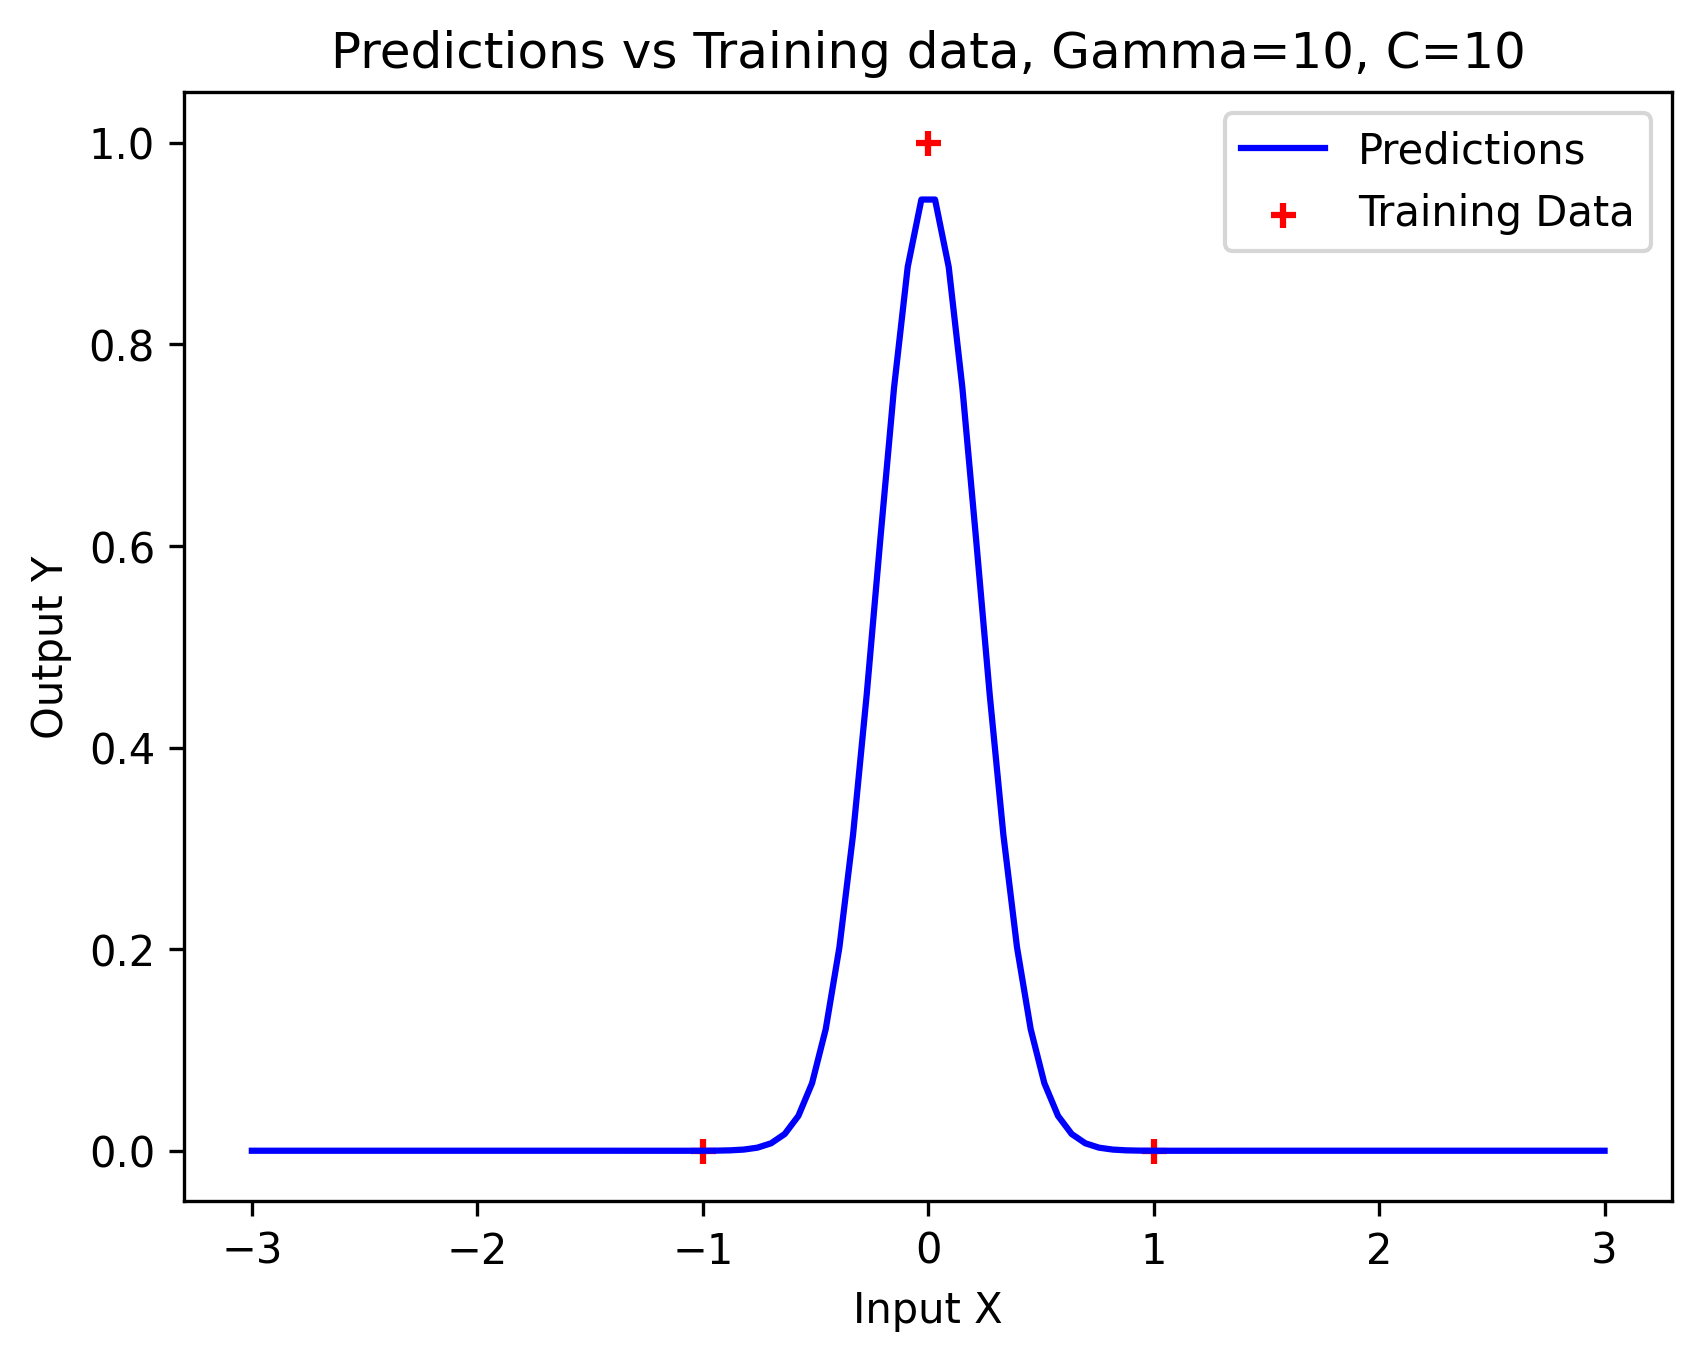
\includegraphics[width=8cm]{kr23.png}}}
\qquad
\subfloat[Gamma = 25, C= 10]{{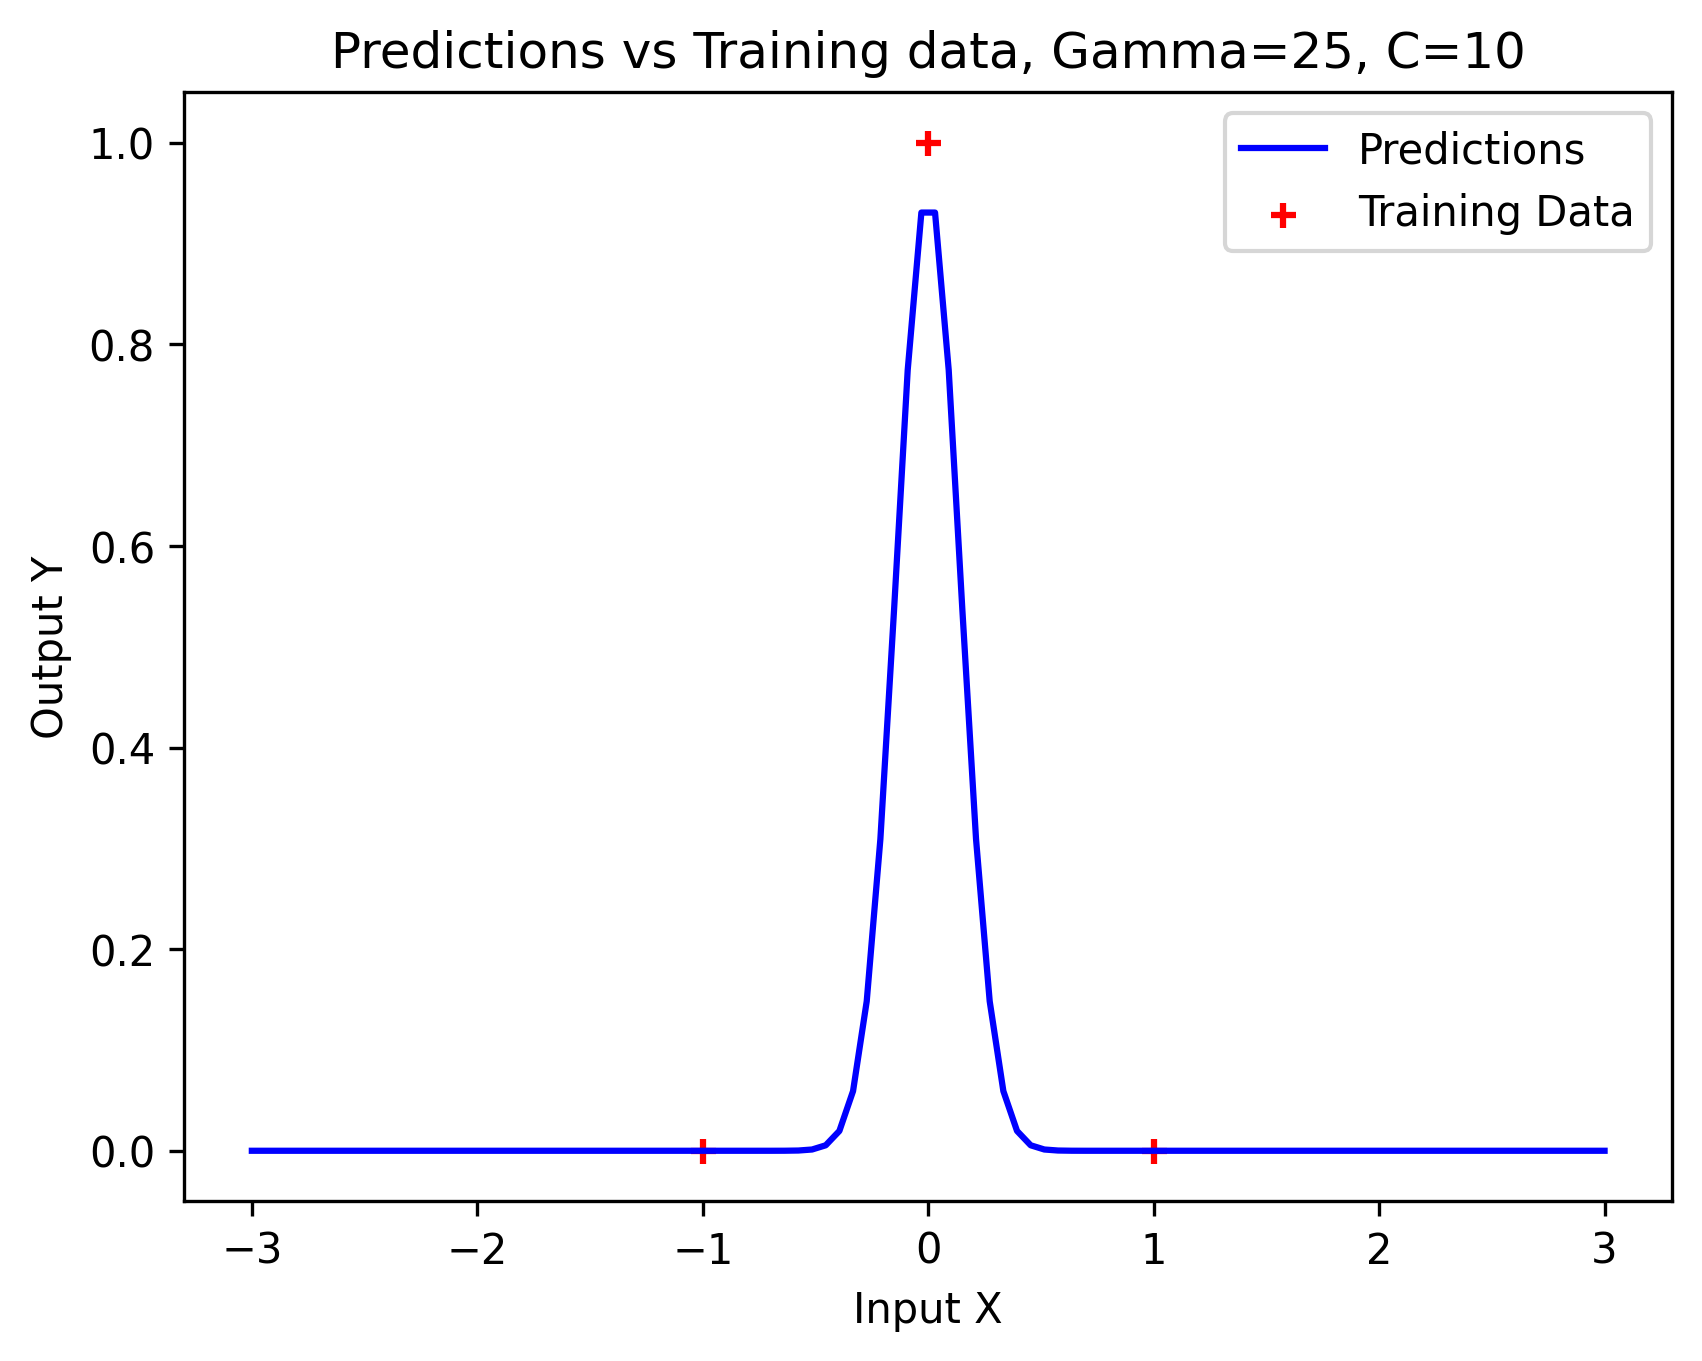
\includegraphics[width=8cm]{kr24.png}}}
\end{figure}
\(\theta_0= -6.5574, \theta_1= 13.4426 , \theta_2= -6.5574\)\\
\(\theta_0= -0.4323, \theta_1= 1.2553 , \theta_2= -0.4323\)\\
\(\theta_0= -0.0061, \theta_1= 0.9525 , \theta_2= -0.0061\)\\
\(\theta_0= -0.0, \theta_1= 0.9524 , \theta_2= -0.0\)\\
\(\theta_0= -0.0, \theta_1= 0.9524 , \theta_2= -0.0\)\\

\begin{figure}[h]
\centering
\subfloat[Gamma = 0, C = 100]{{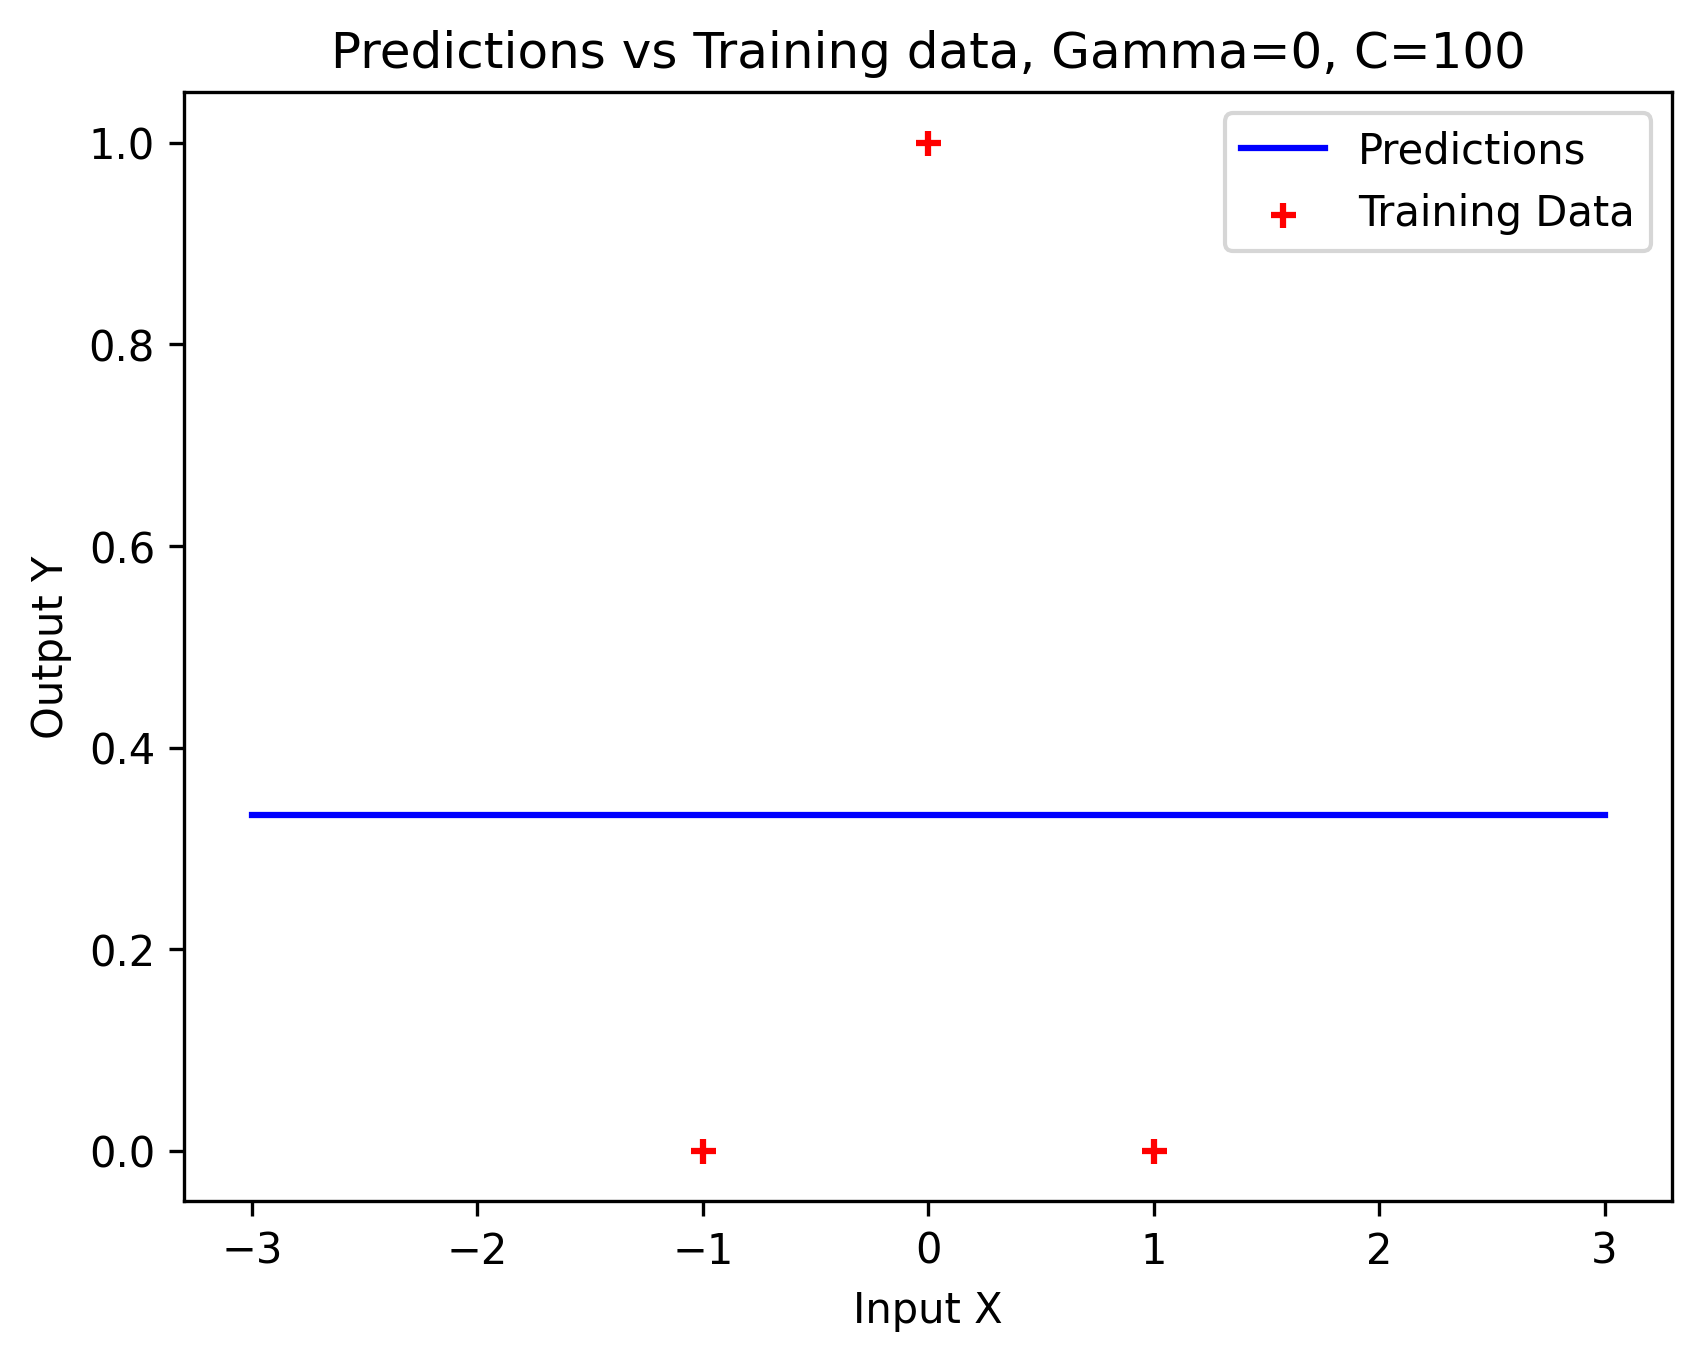
\includegraphics[width=8cm]{kr30.png}}}
\qquad
\subfloat[Gamma = 1, C = 100]{{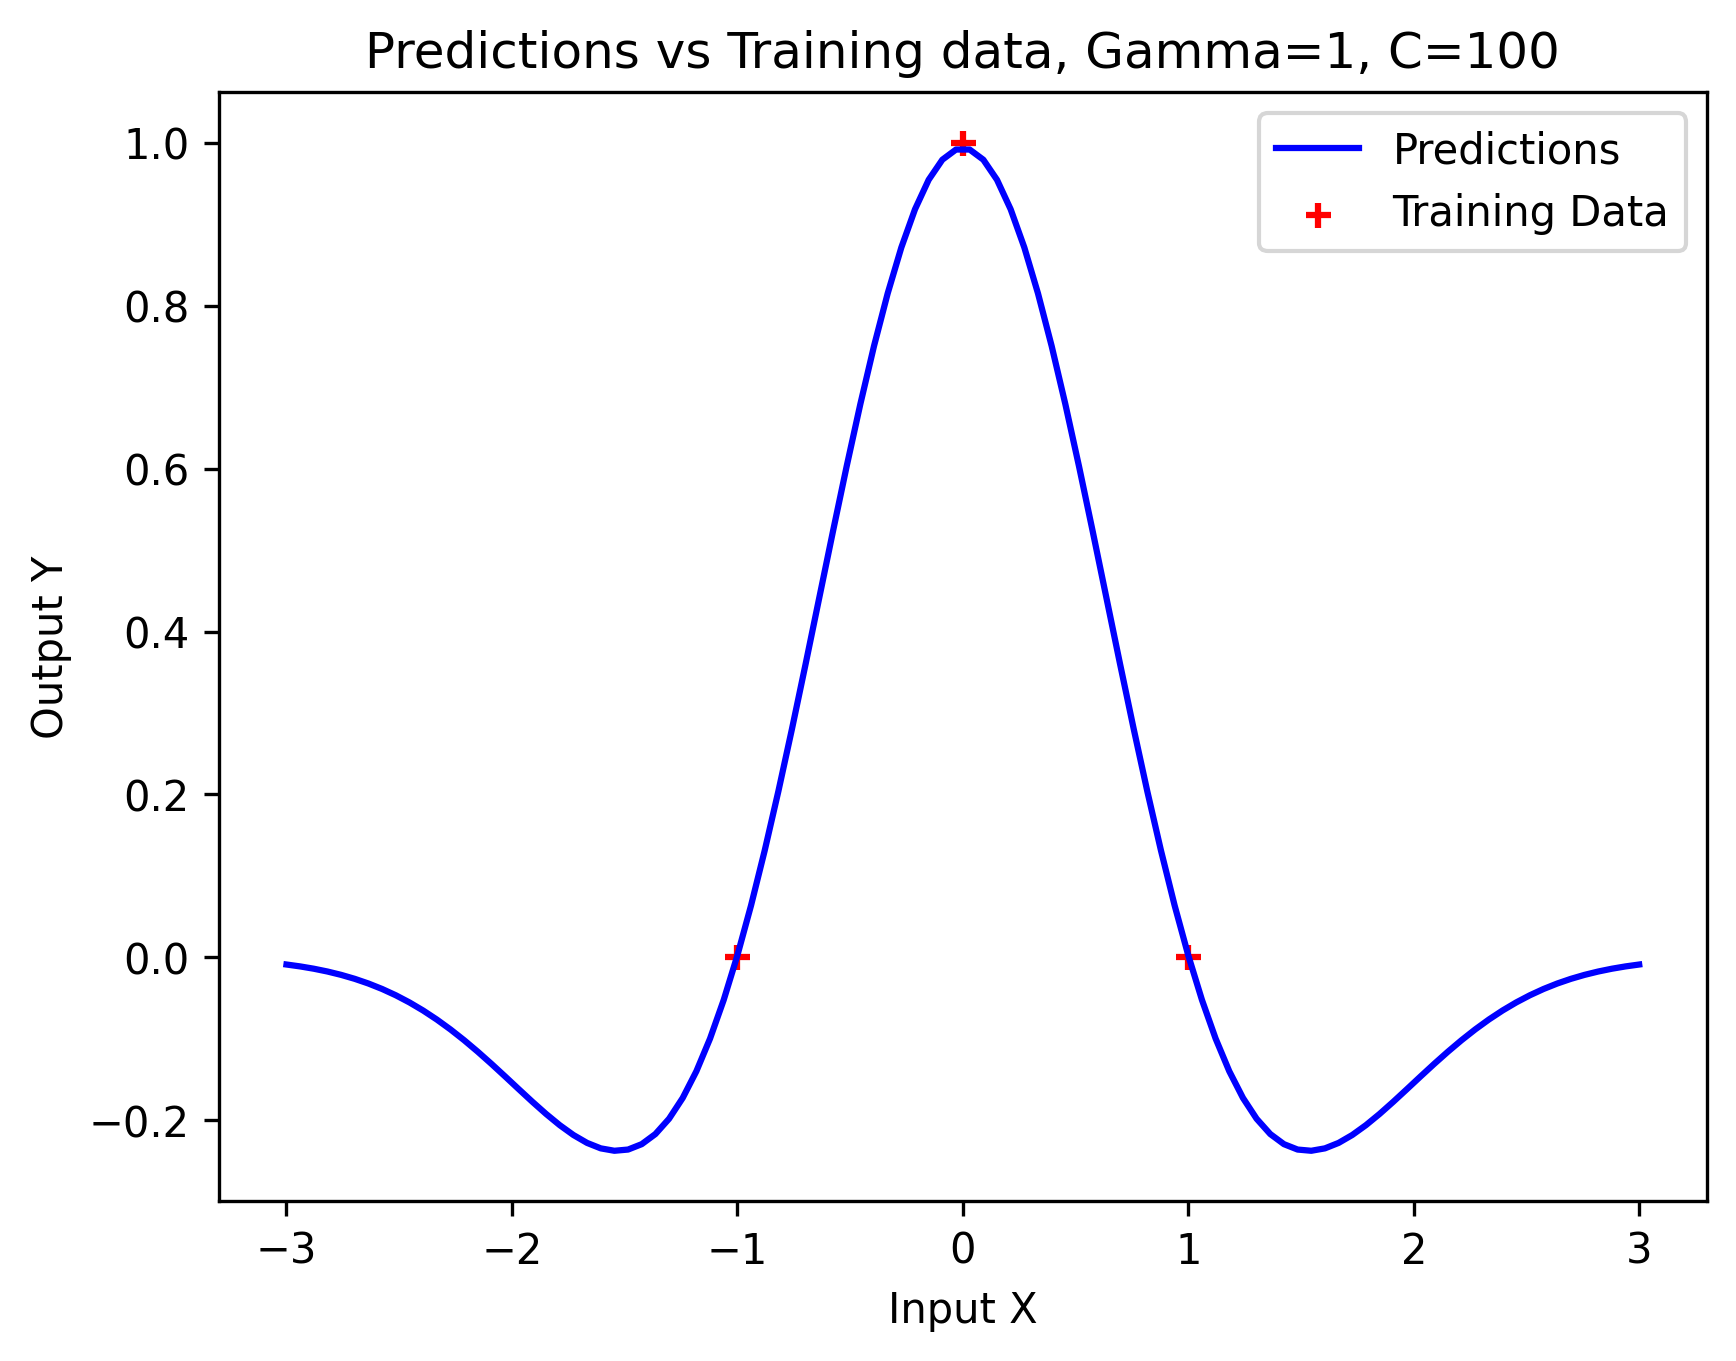
\includegraphics[width=8cm]{kr31.png}}}
\qquad
\subfloat[Gamma = 5, C= 100]{{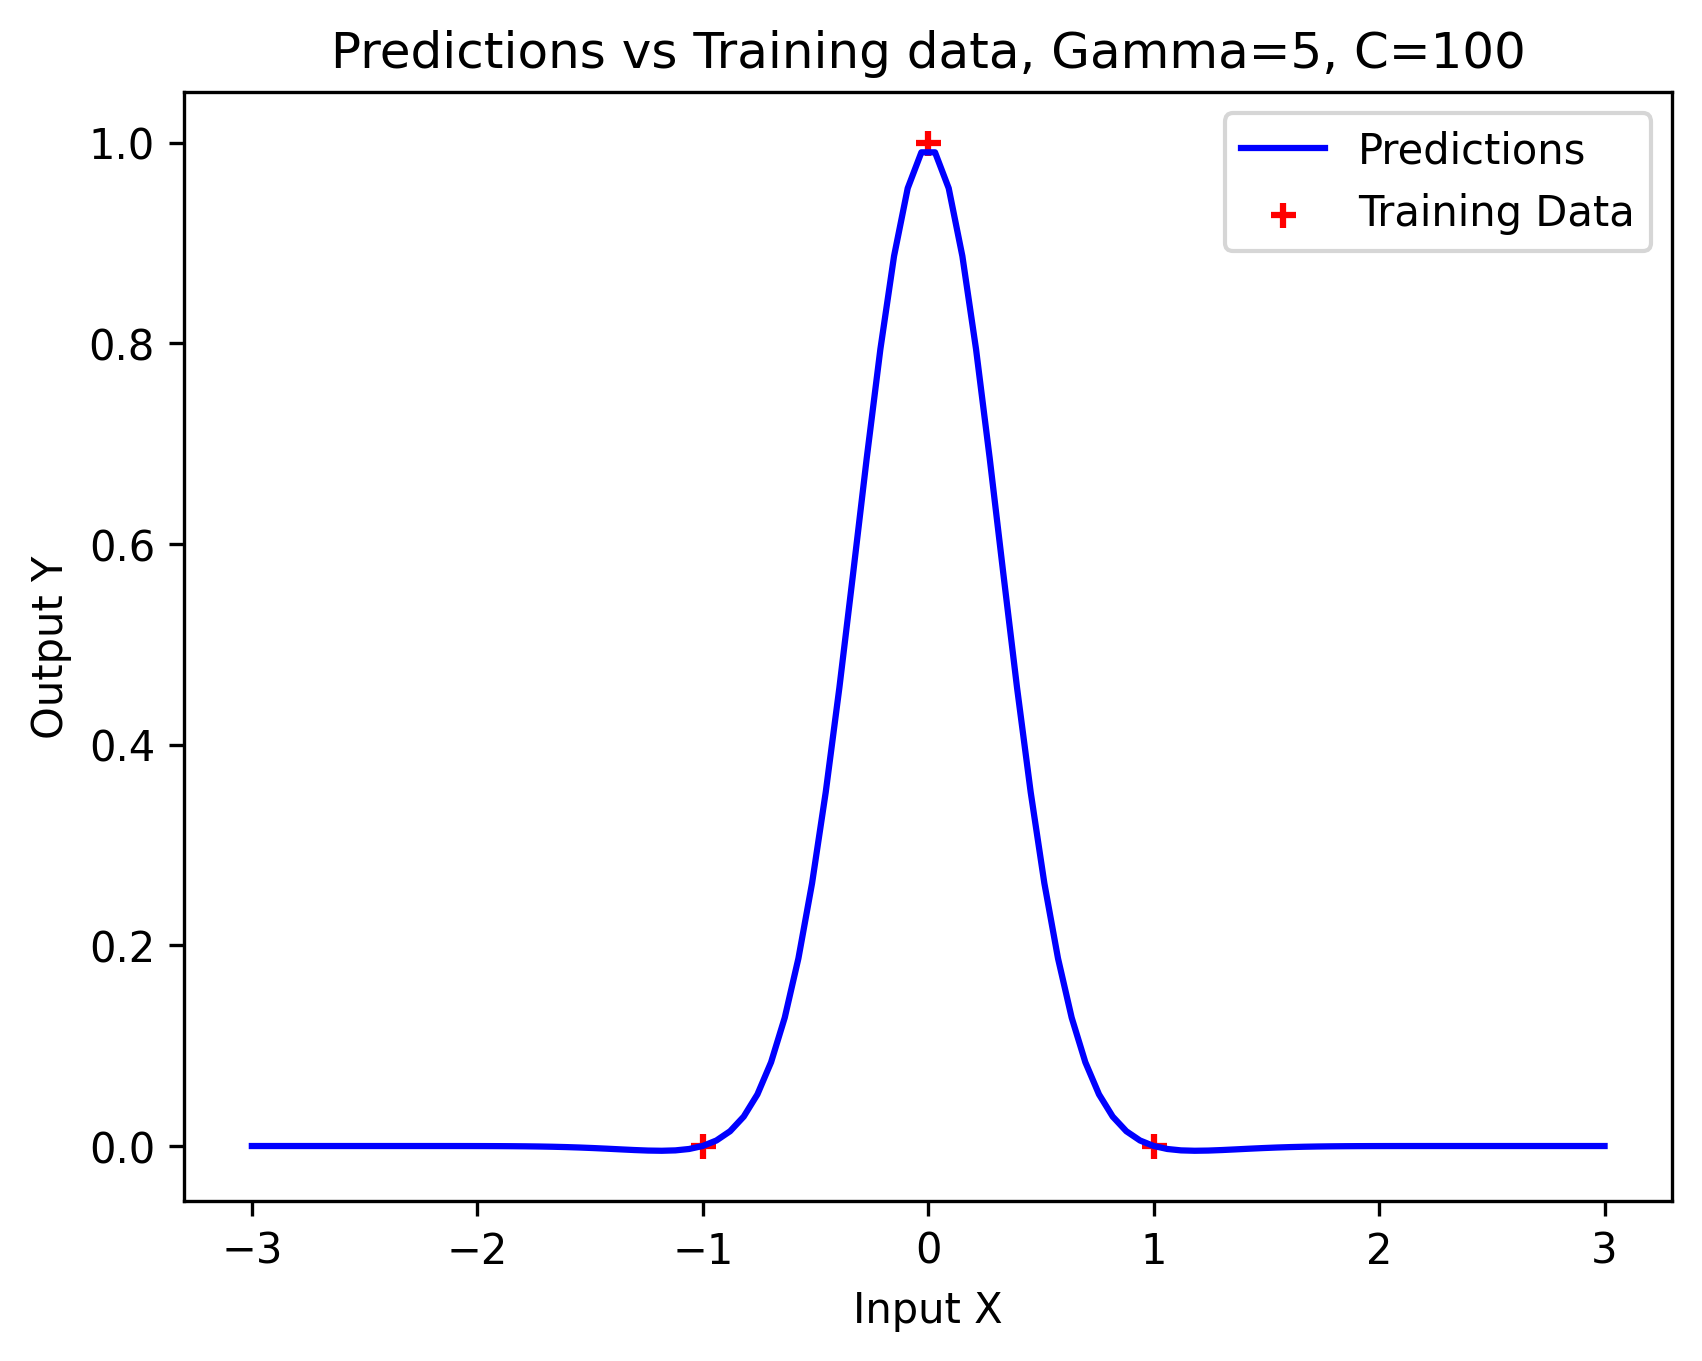
\includegraphics[width=8cm]{kr32.png}}}
\qquad
\subfloat[Gamma = 10, C= 100]{{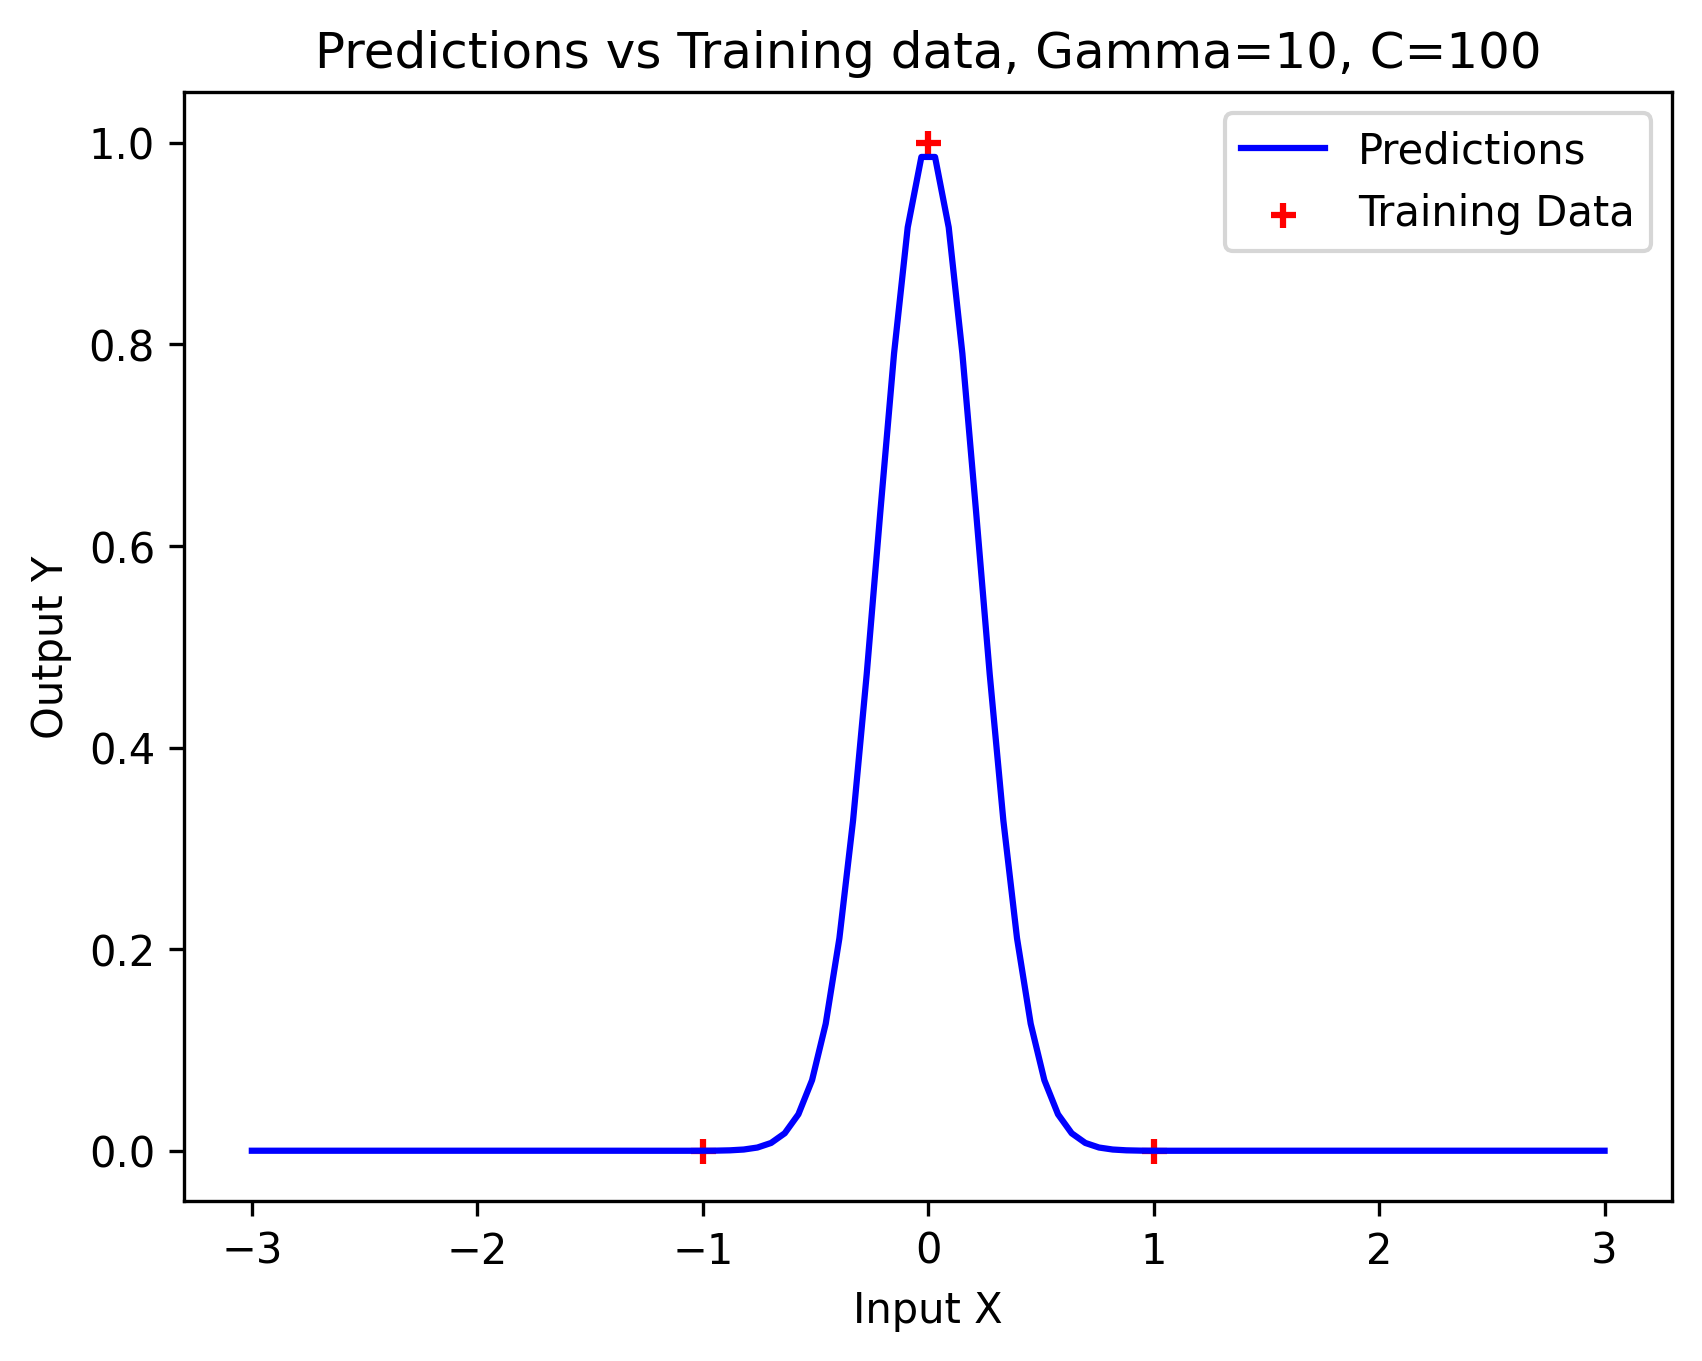
\includegraphics[width=8cm]{kr33.png}}}
\qquad
\subfloat[Gamma = 25, C= 100]{{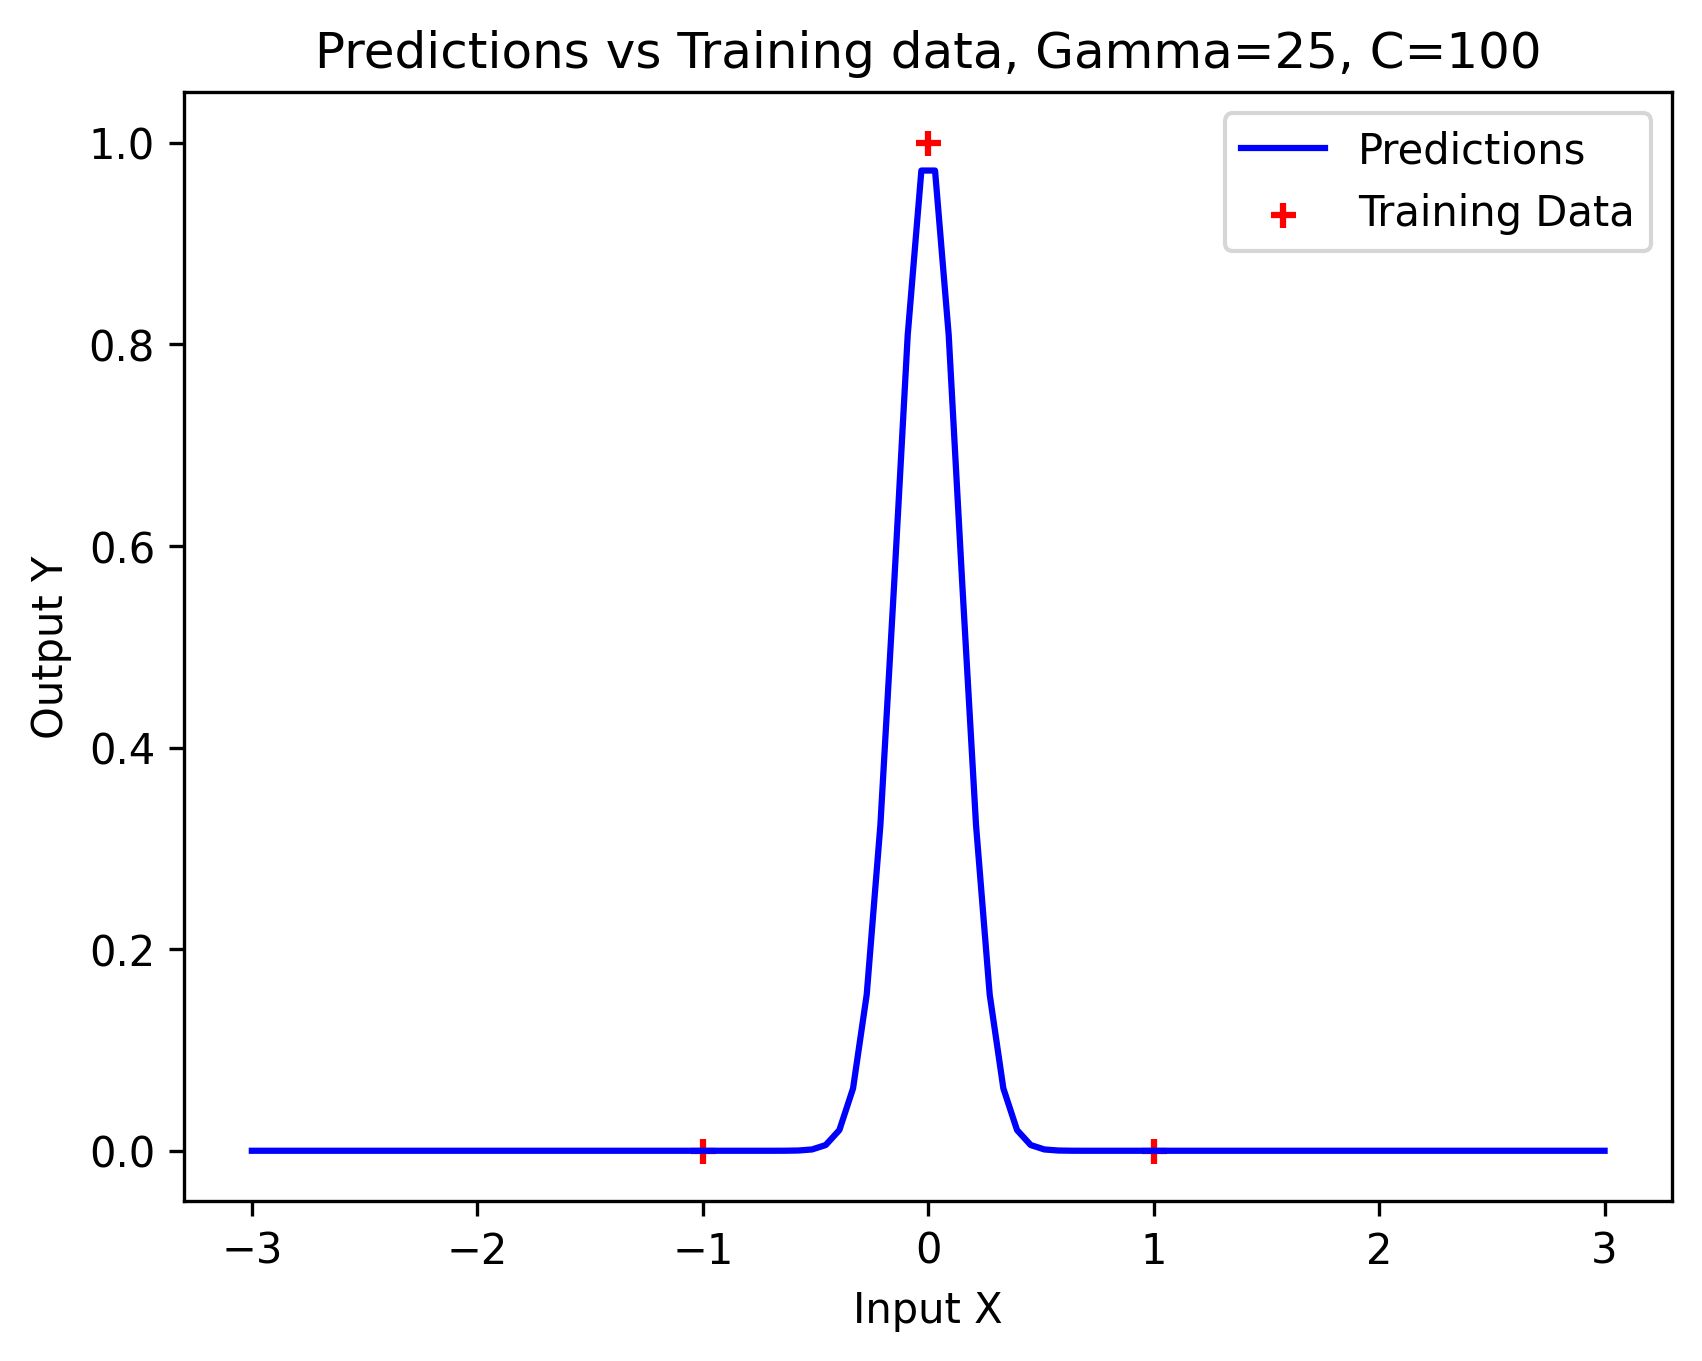
\includegraphics[width=8cm]{kr34.png}}}
\end{figure}
\(\theta_0= -66.5557, \theta_1= 133.4443 , \theta_2= -66.5557\)\\
\(\theta_0= -0.4855, \theta_1= 1.3504 , \theta_2= -0.4855\)\\
\(\theta_0= -0.0067, \theta_1= 0.9951 , \theta_2= -0.0067\)\\
\(\theta_0= -0.0, \theta_1= 0.995 , \theta_2= -0.0\)\\
\(\theta_0= -0.0, \theta_1= 0.995 , \theta_2= -0.0\)\\

\begin{figure}[h]
\centering
\subfloat[Gamma = 0, C = 1000]{{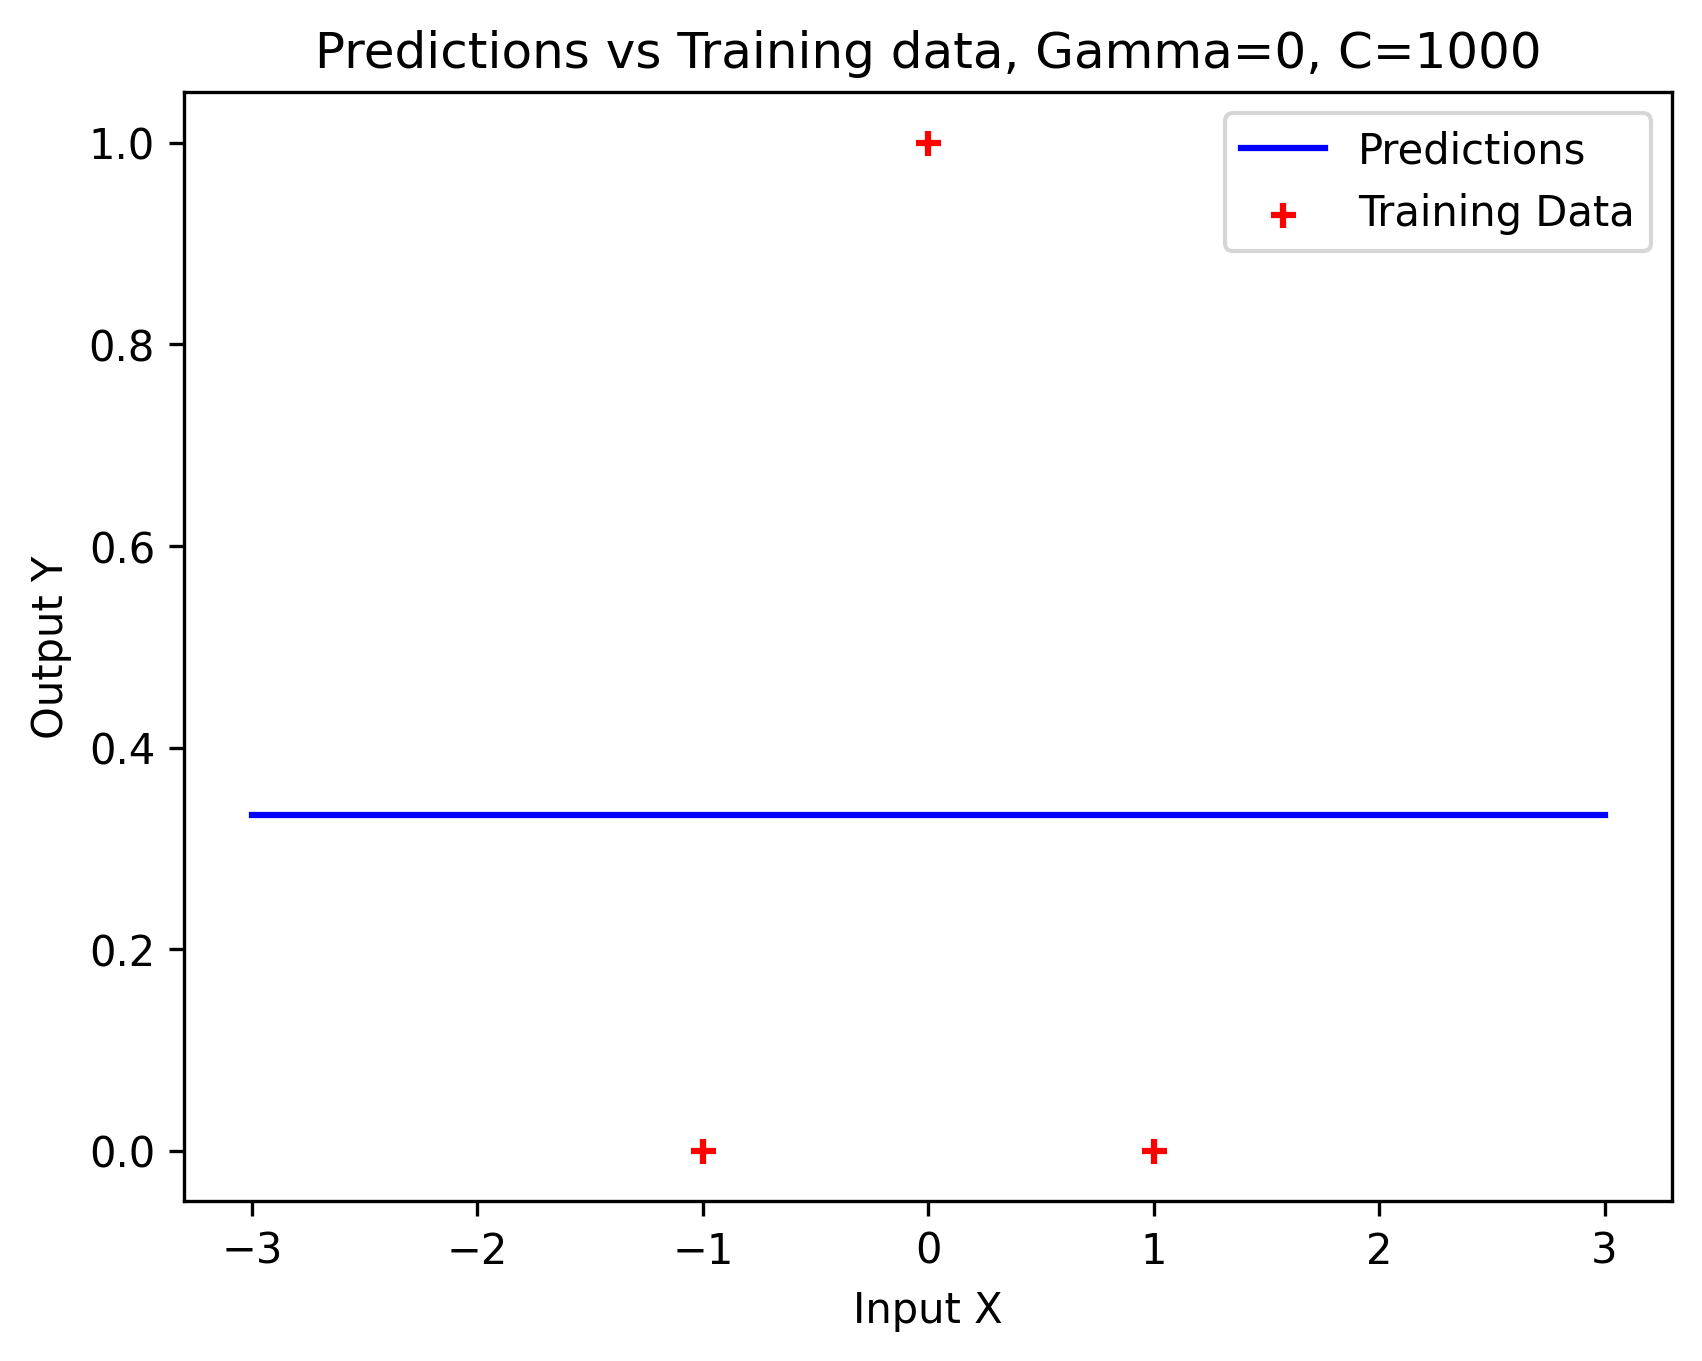
\includegraphics[width=8cm]{kr40.png}}}
\qquad
\subfloat[Gamma = 1, C = 1000]{{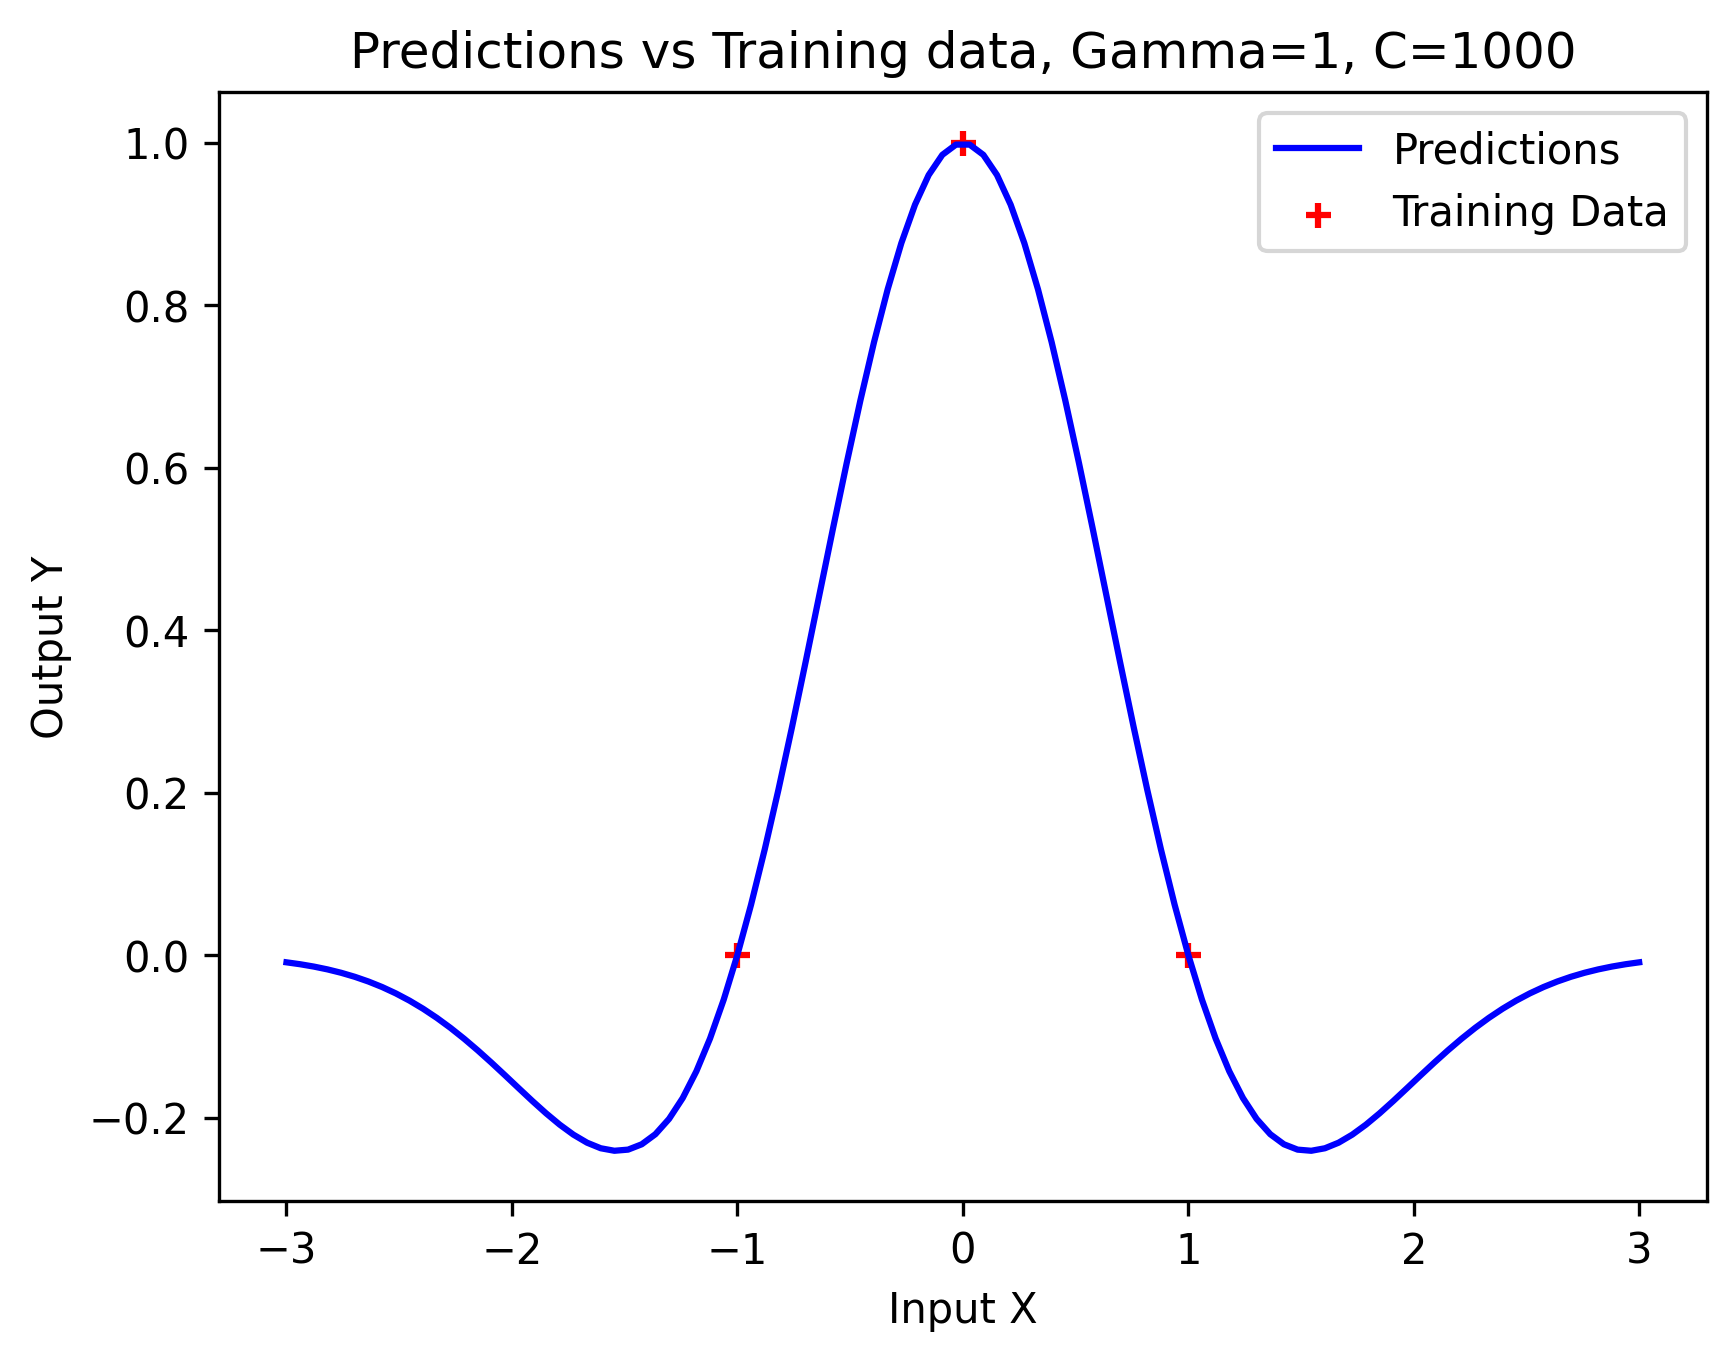
\includegraphics[width=8cm]{kr41.png}}}
\qquad
\subfloat[Gamma = 5, C= 1000]{{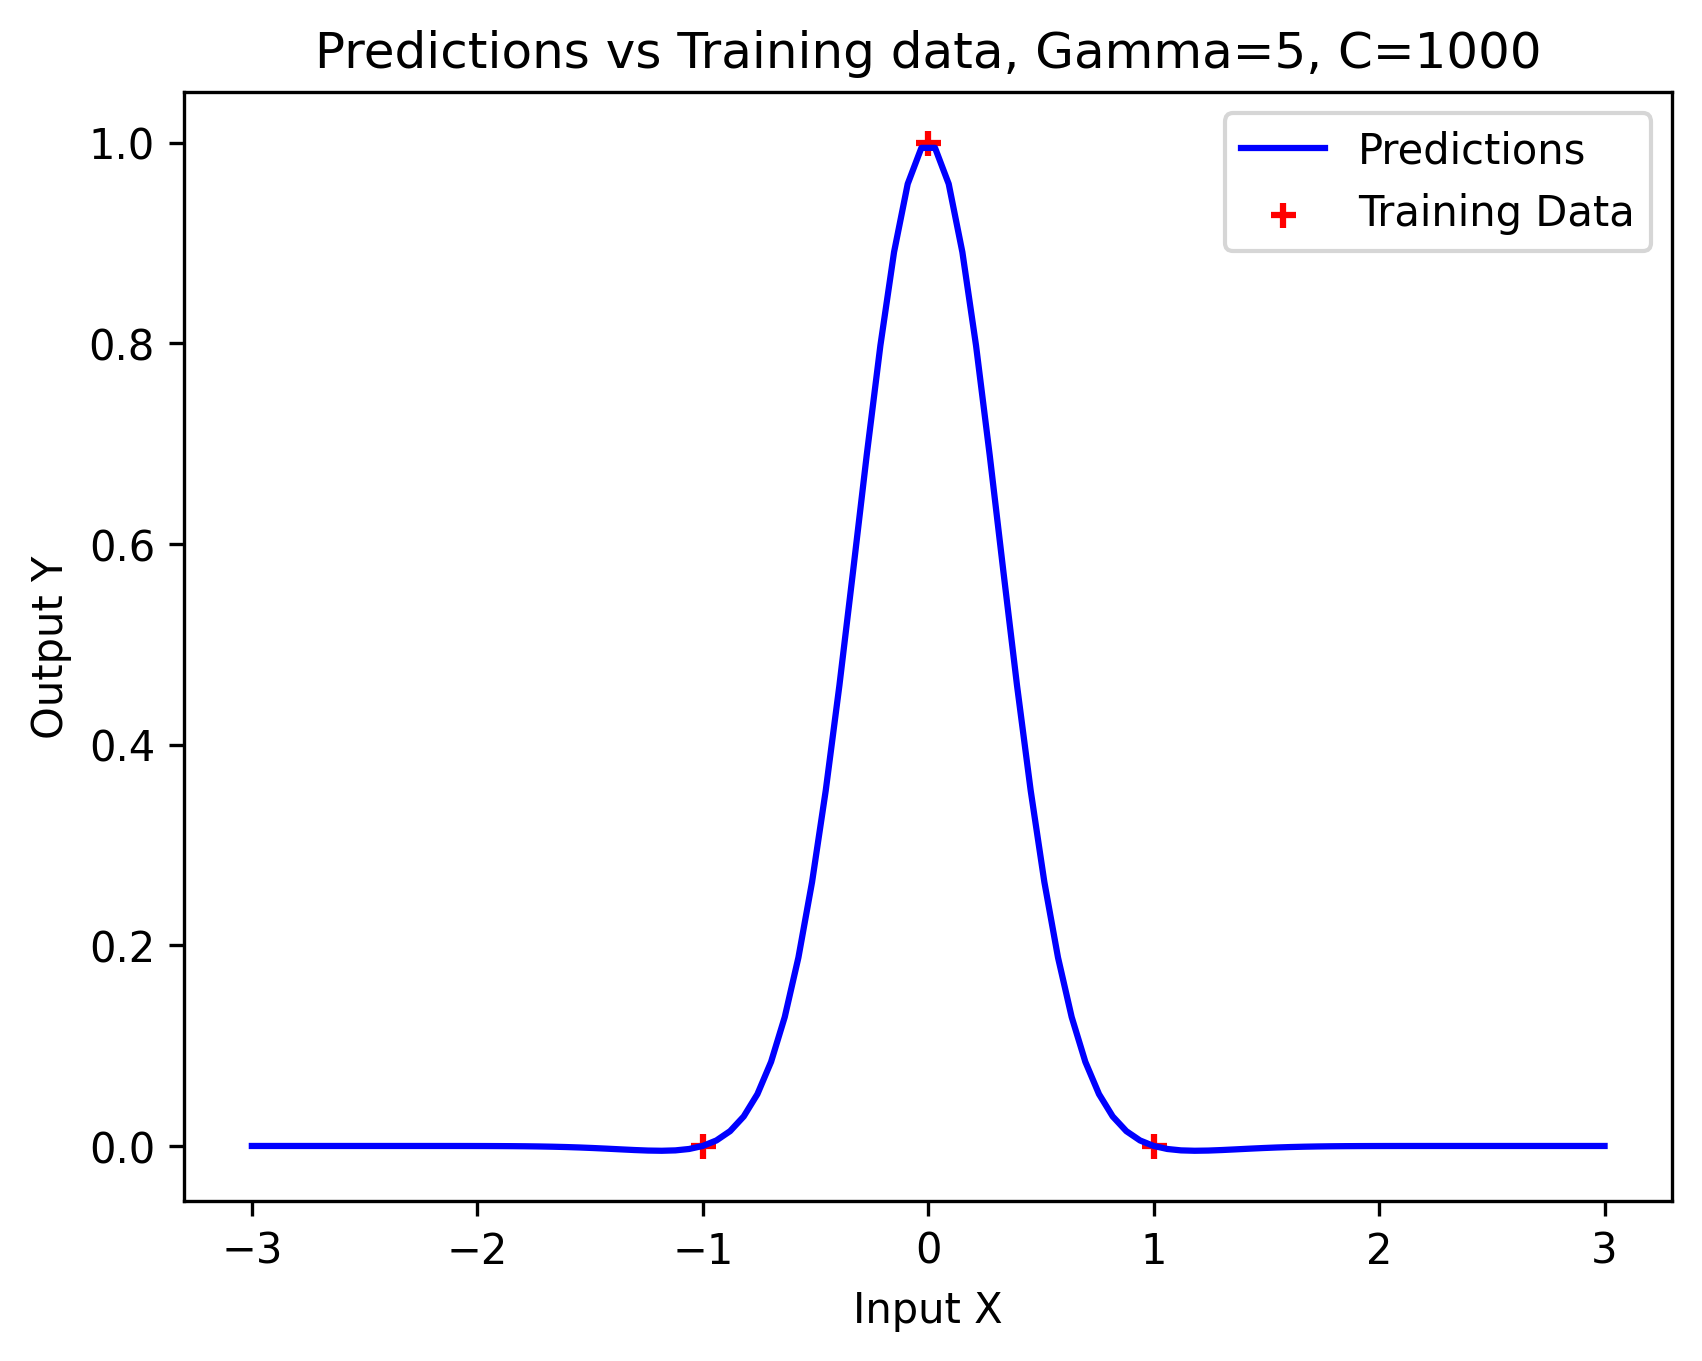
\includegraphics[width=8cm]{kr42.png}}}
\qquad
\subfloat[Gamma = 10, C= 1000]{{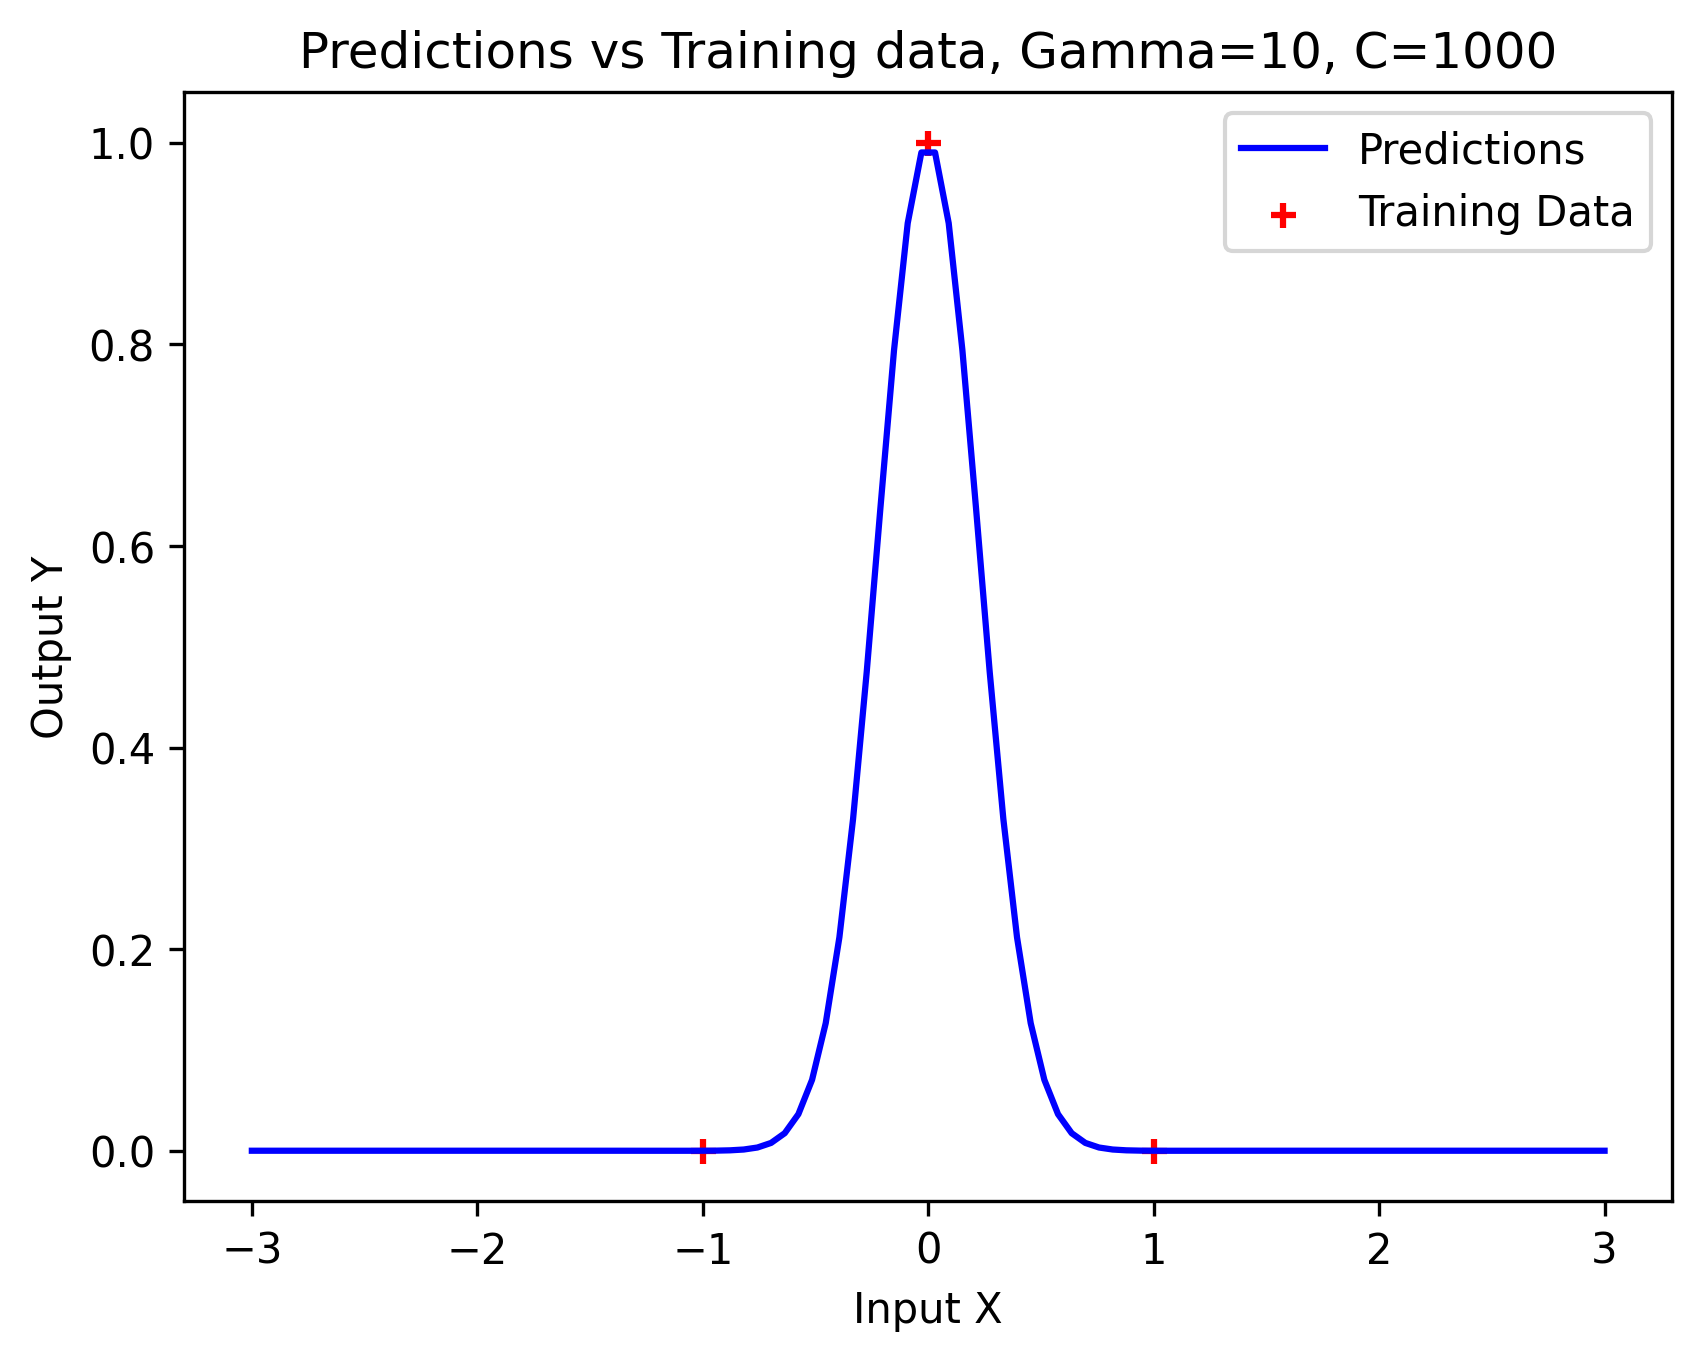
\includegraphics[width=8cm]{kr43.png}}}
\qquad
\subfloat[Gamma = 25, C= 1000]{{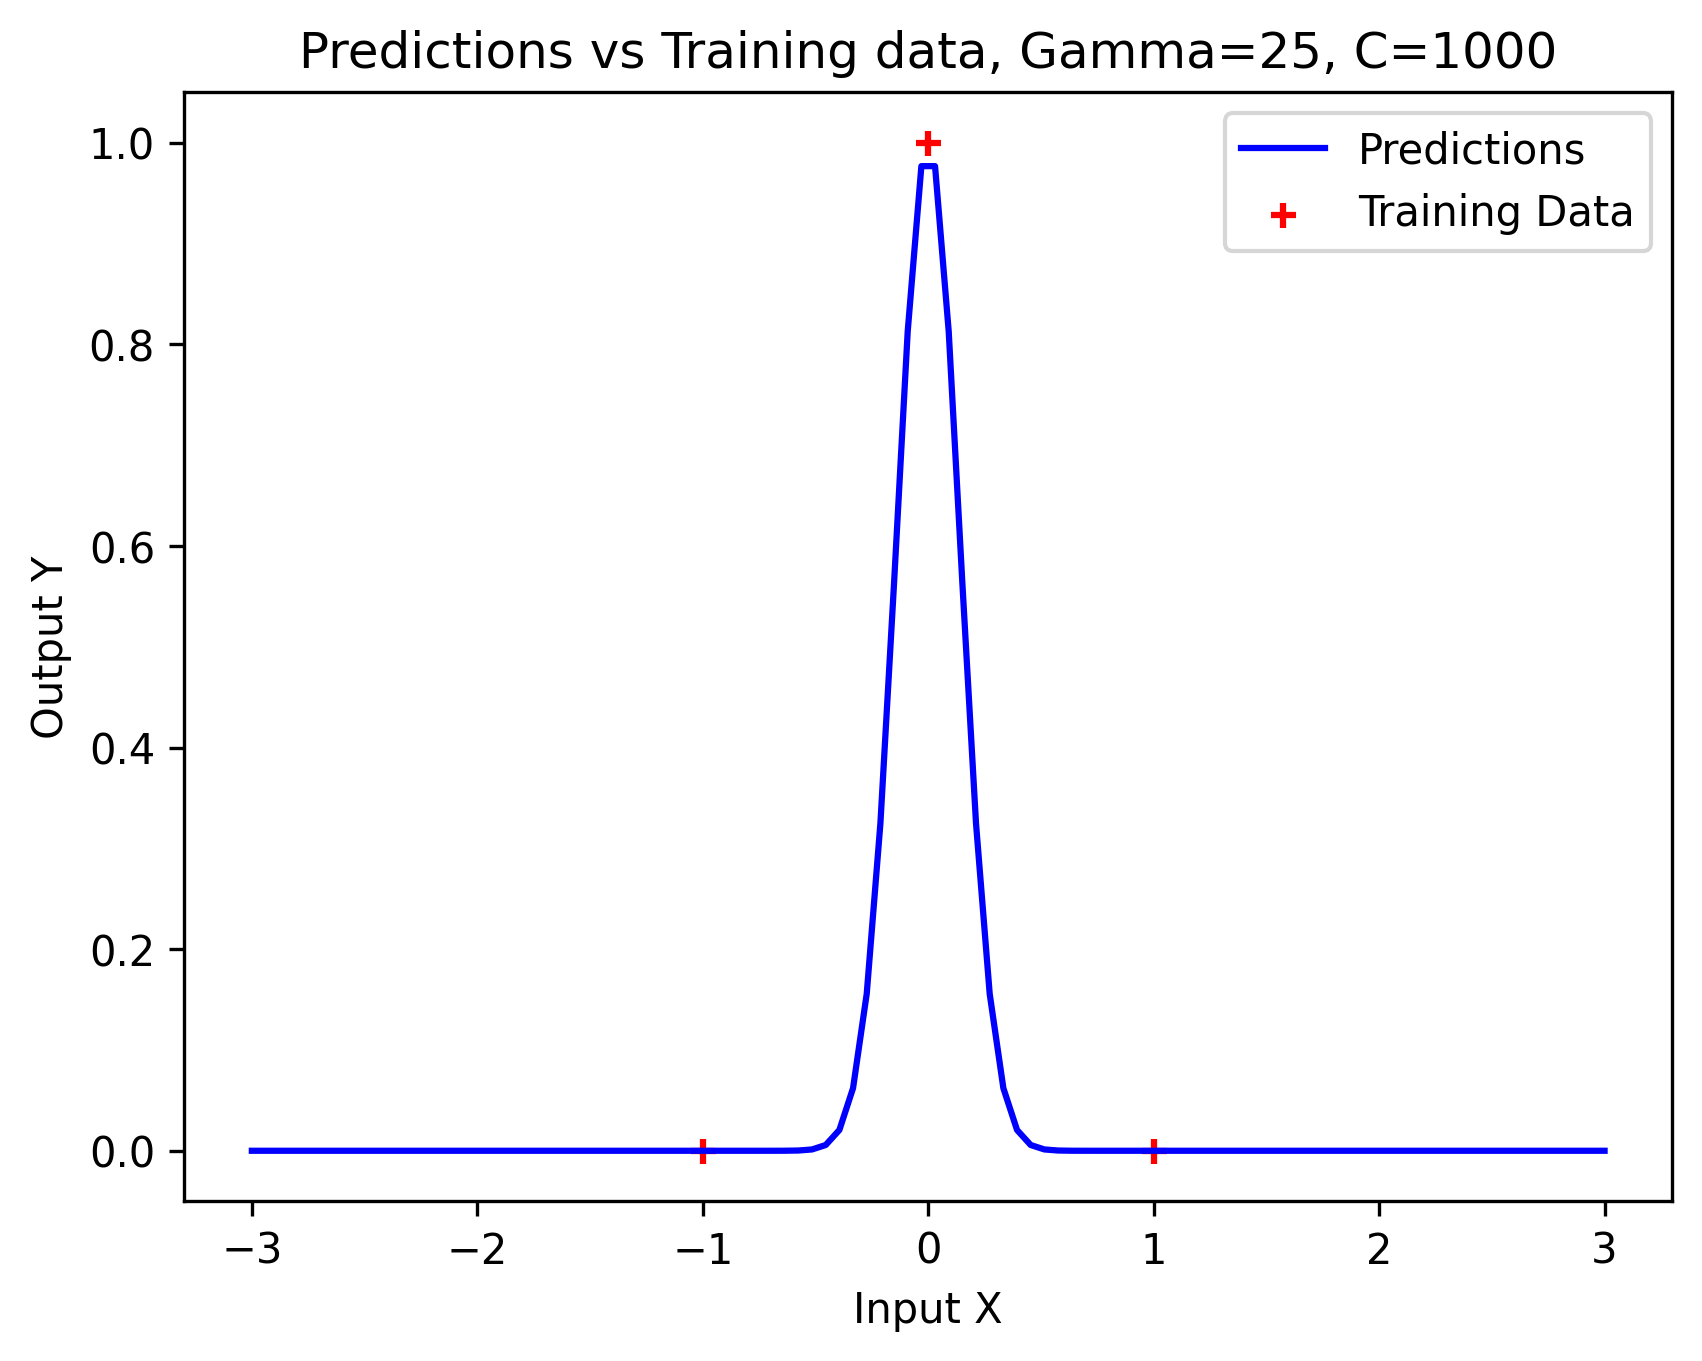
\includegraphics[width=8cm]{kr44.png}}}
\end{figure}
\(\theta_0= -666.5556, \theta_1= 1333.4444 , \theta_2= -666.5556\)\\
\(\theta_0= -0.4914, \theta_1= 1.3609 , \theta_2= -0.4914\)\\
\(\theta_0= -0.0067, \theta_1= 0.9996 , \theta_2= -0.0067\)\\
\(\theta_0= -0.0, \theta_1= 0.9995 , \theta_2= -0.0\)\\
\(\theta_0= -0.0, \theta_1= 0.9995 , \theta_2= -0.0\)\\

\clearpage
\subsection{D}
Kernalised Ridge Regression works by applying a L2 penalty to normal linear regression to shrink parameters down to near 0 that aren't as important to the model in an effort to prevent overfitting. This used along side a kernel can introduce non-linearity to the regressor by introducing new features that are non-linear depending on the type of kernel used. In this case we use a Gaussian kernel to introduce new features hence enabling us to fit a non-linear curve to our data. When we vary our values of C and Gamma, we alter how much of a penalty does the L2 penalty give and also alter how much each of our new features introduced by our kernel effects the slope of our curve. From our data we can see that lower values of Gamma give us much more curved predictions while higher values of gamma snap to the data points. Lower values of C allow for much more of our data to be underfitted while higher values of C do not. When we take these 2 together, Gamma gives us the slope of our line due to introducing non-linear features while C reigns in the slope by giving a penalty to parameters that are not as important in dictating the slope of our line. We can see this in our data, as our value of Gamma is increasing, C gives a more strict penalty hence why more of out parameters are approaching 0(I've rounded the data).  In terms of behaviour between KNN and Kernalised Ridge Regression, Kernalised Ridge Regression allows for more flexible models overall as we can tune both C and Gamma, whiles in KNN we can only tune Gamma. This leads to better predictions as we can get more general and flexible models. KNN seems to much more readily snap to data and give a range of data the same Y output whilst for the same value of Gamma in KRR, it's more general. 
\clearpage

\section{(ii)}
\subsection{A}
\begin{figure}[h]
\centering
\subfloat[Gamma = 0]{{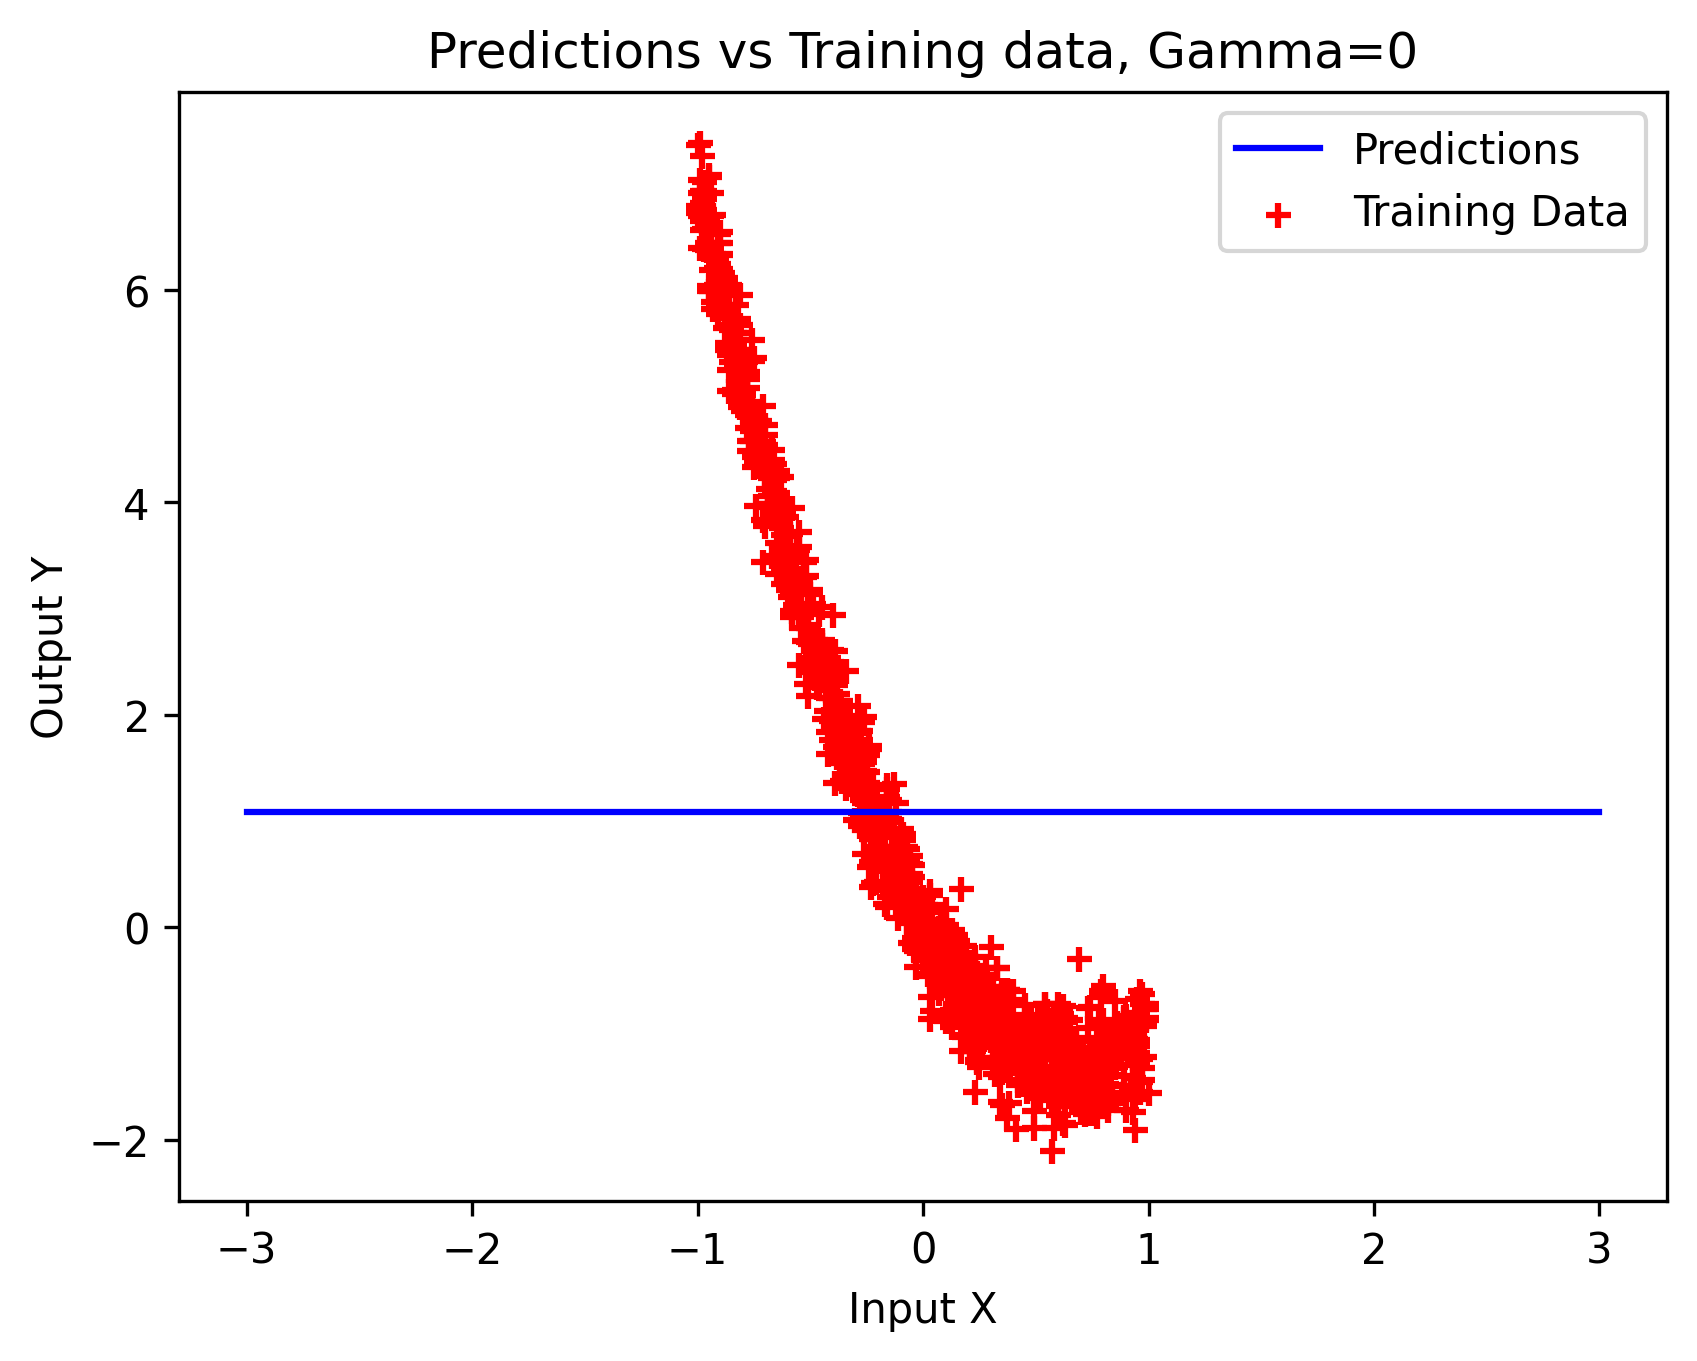
\includegraphics[width=8cm]{ks0.png}}}
\qquad
\subfloat[Gamma = 1]{{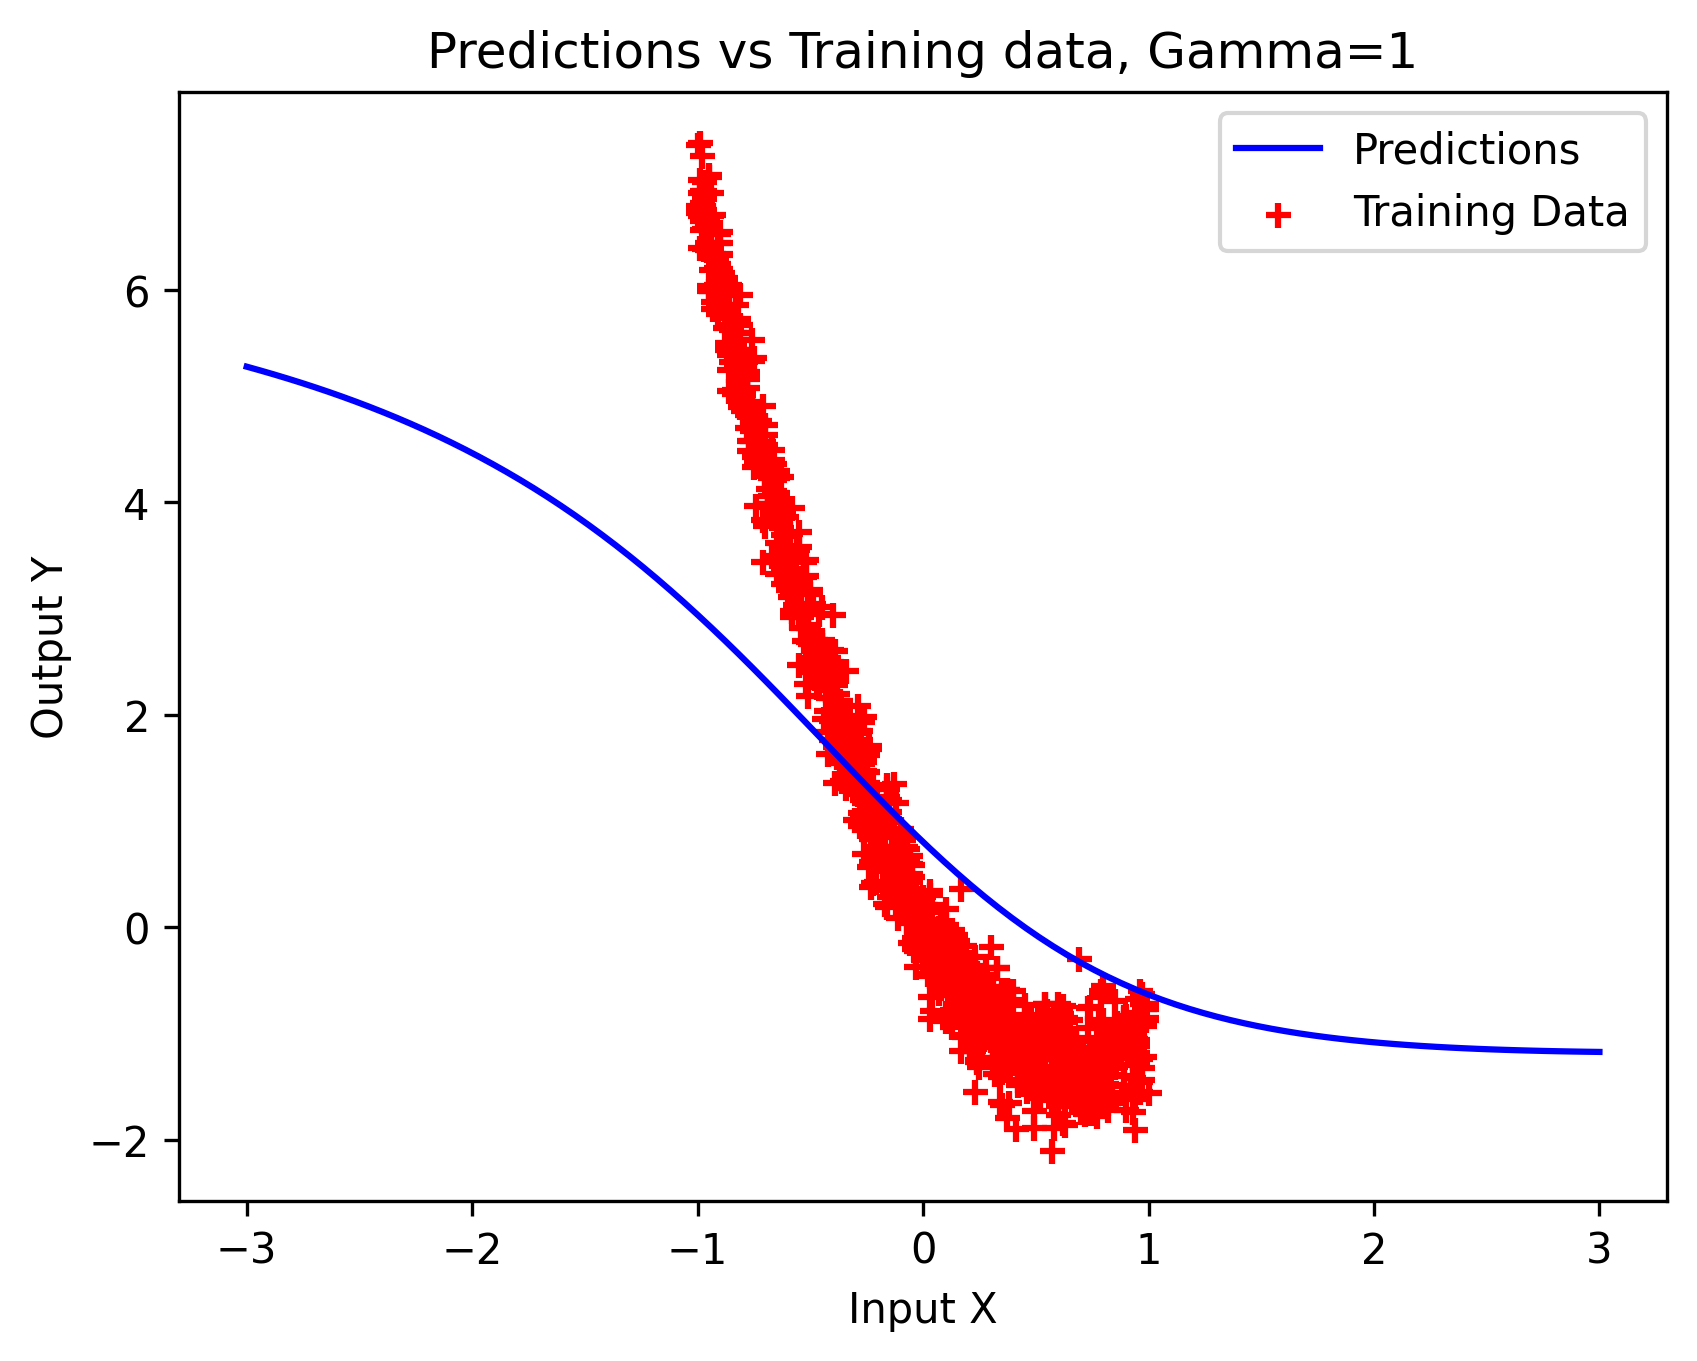
\includegraphics[width=8cm]{ks1.png}}}
\qquad
\subfloat[Gamma = 5]{{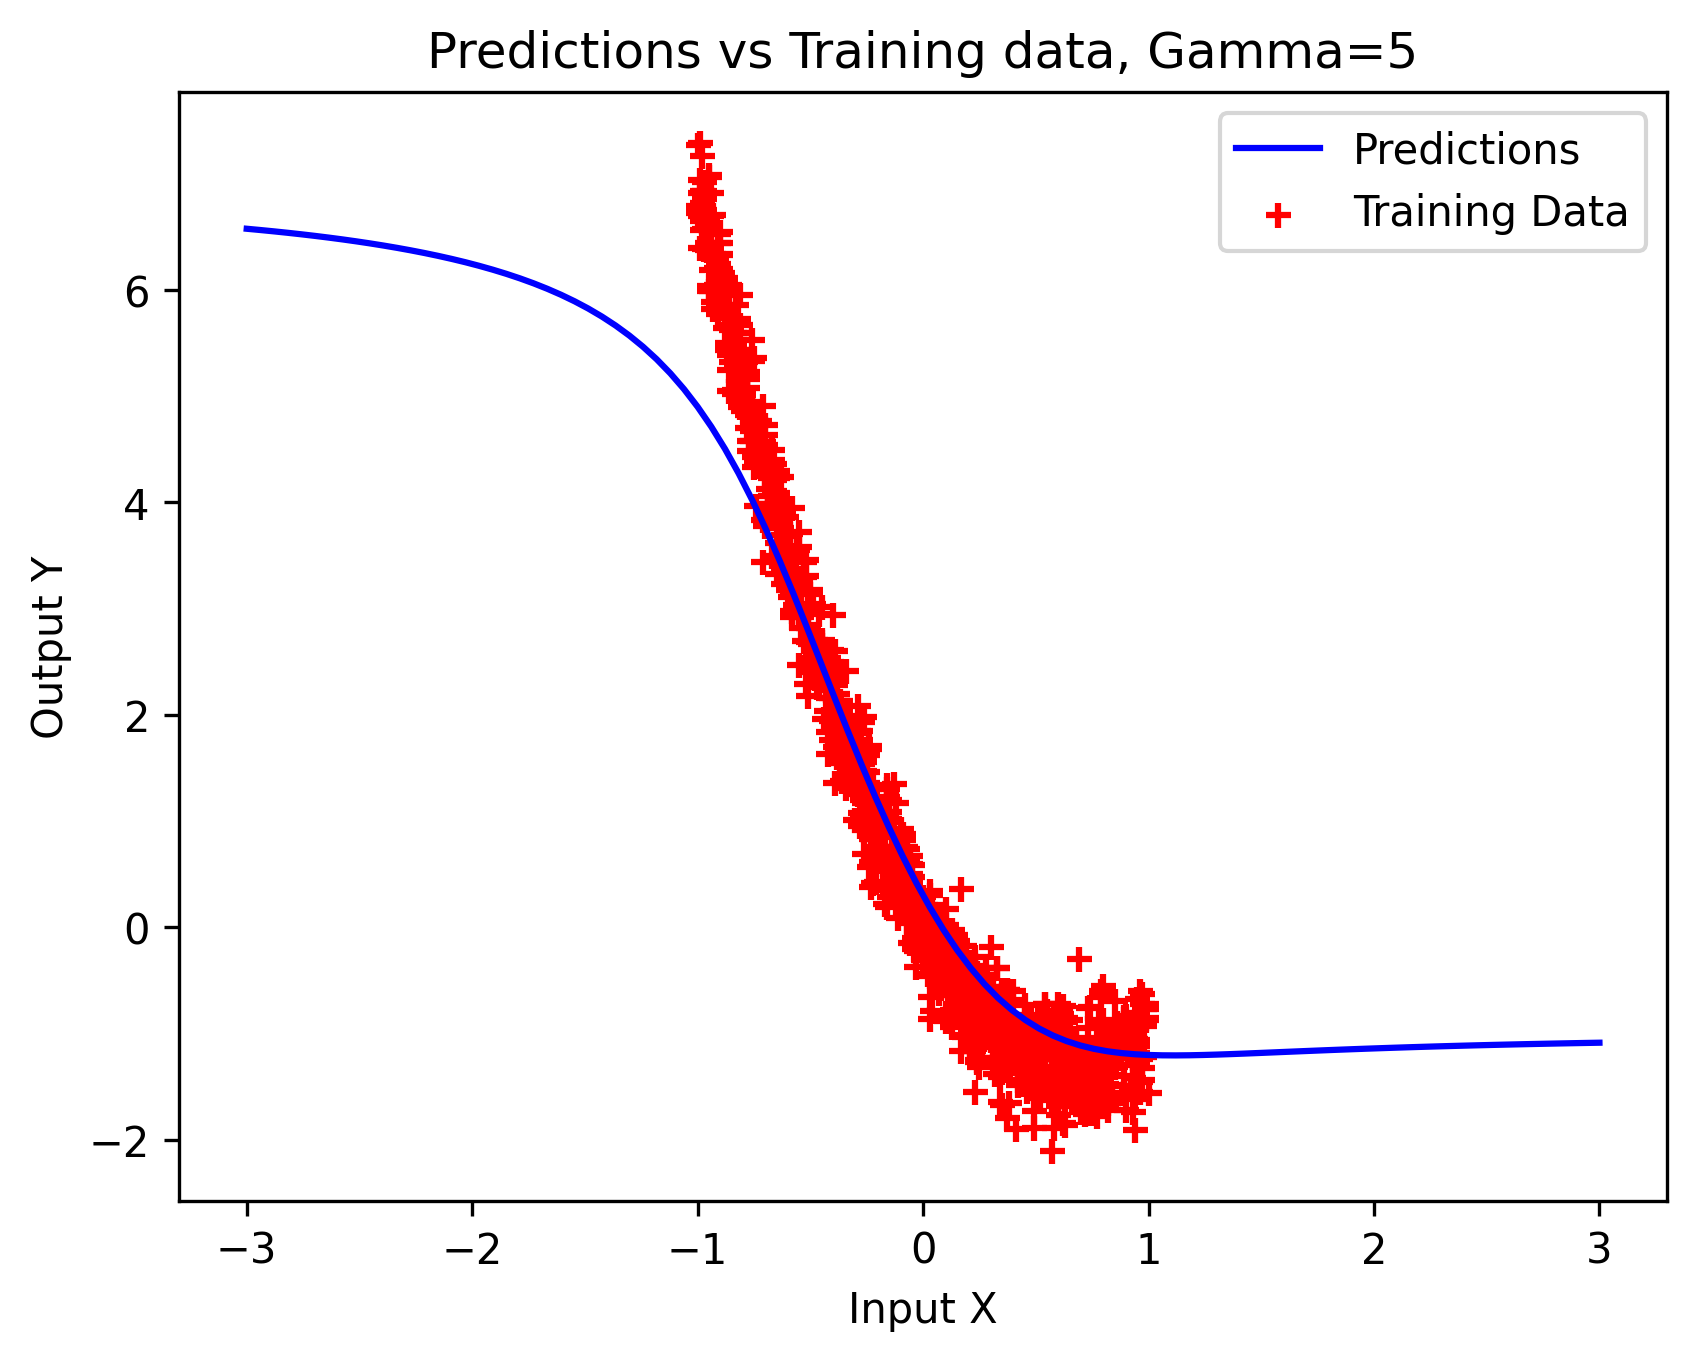
\includegraphics[width=8cm]{ks2.png}}}
\qquad
\subfloat[Gamma = 10]{{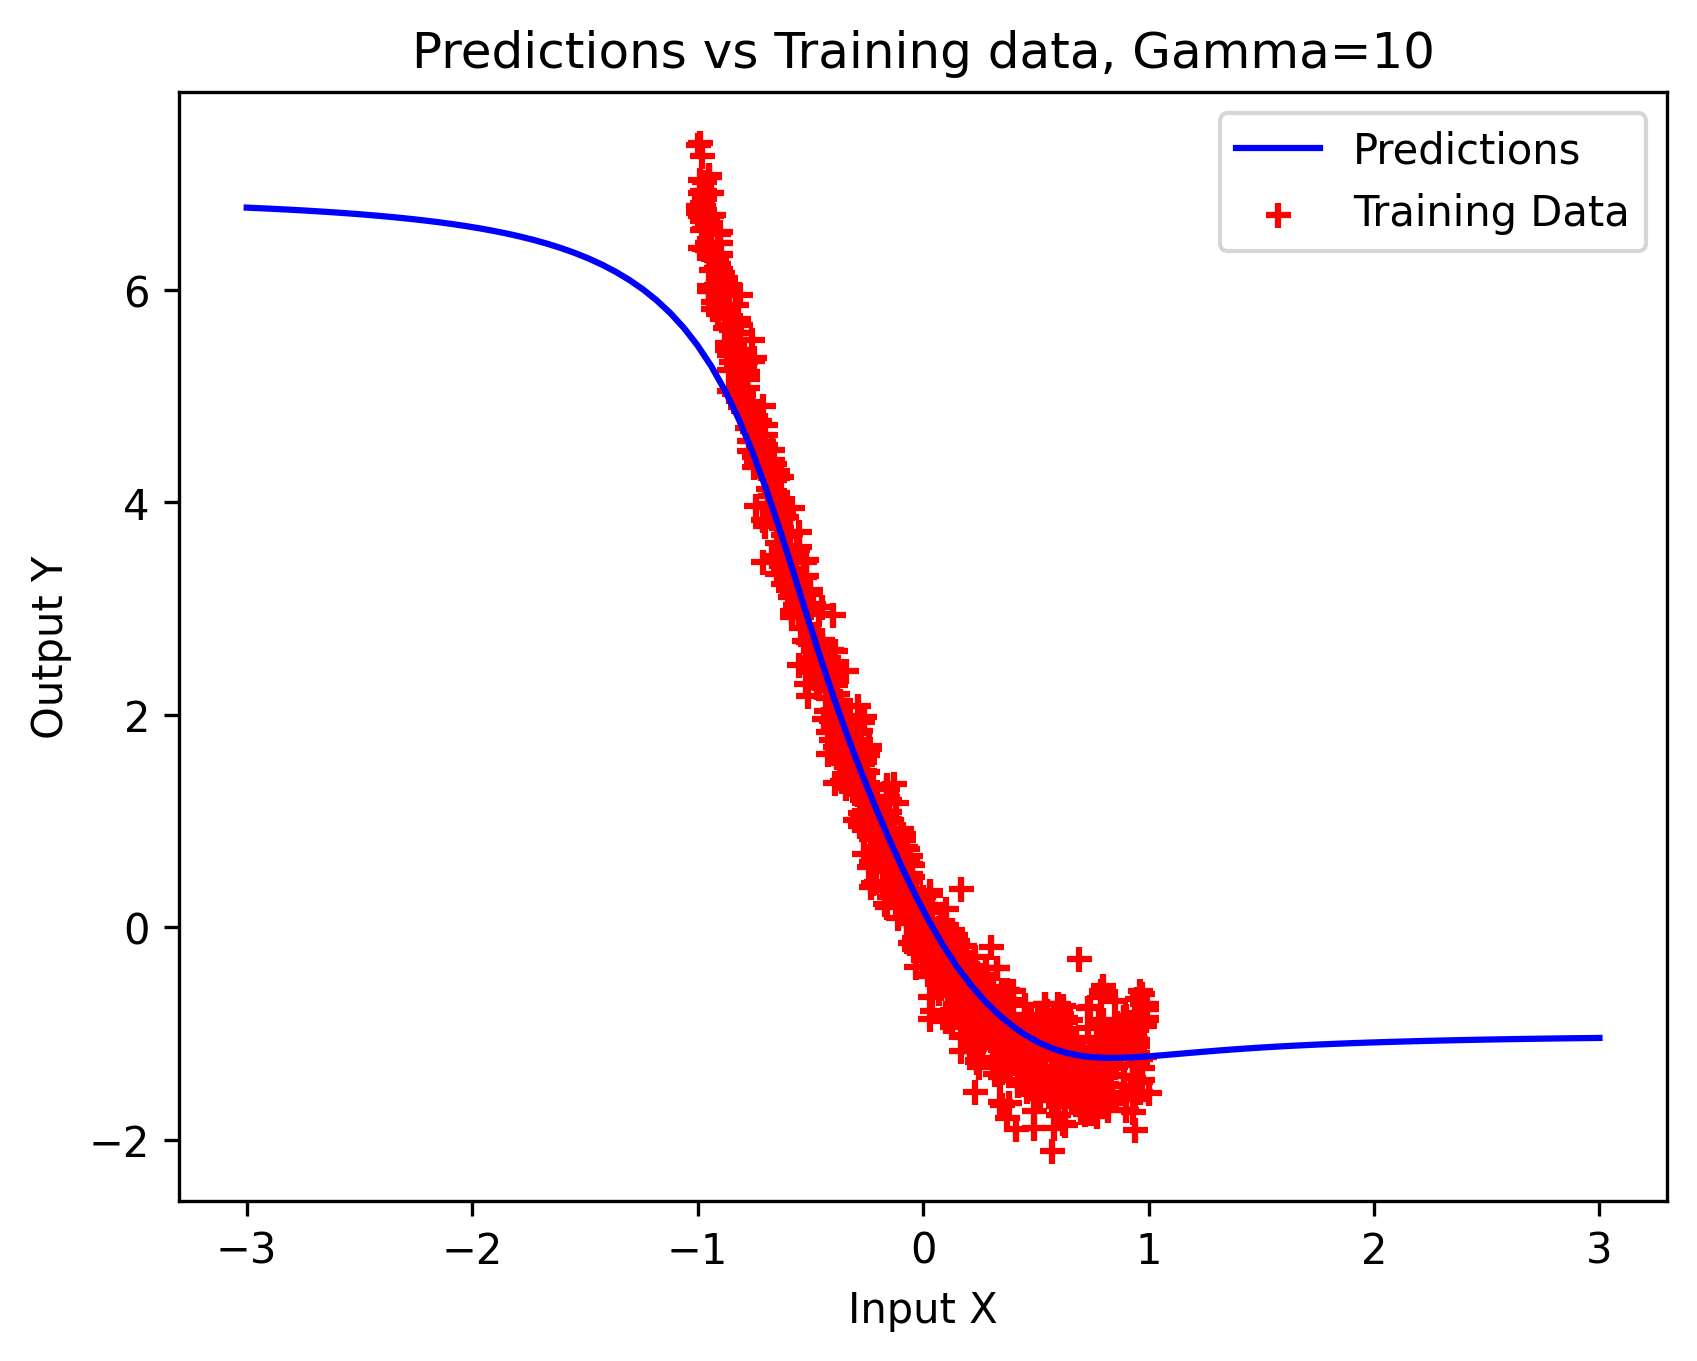
\includegraphics[width=8cm]{ks3.png}}}
\qquad
\subfloat[Gamma = 25]{{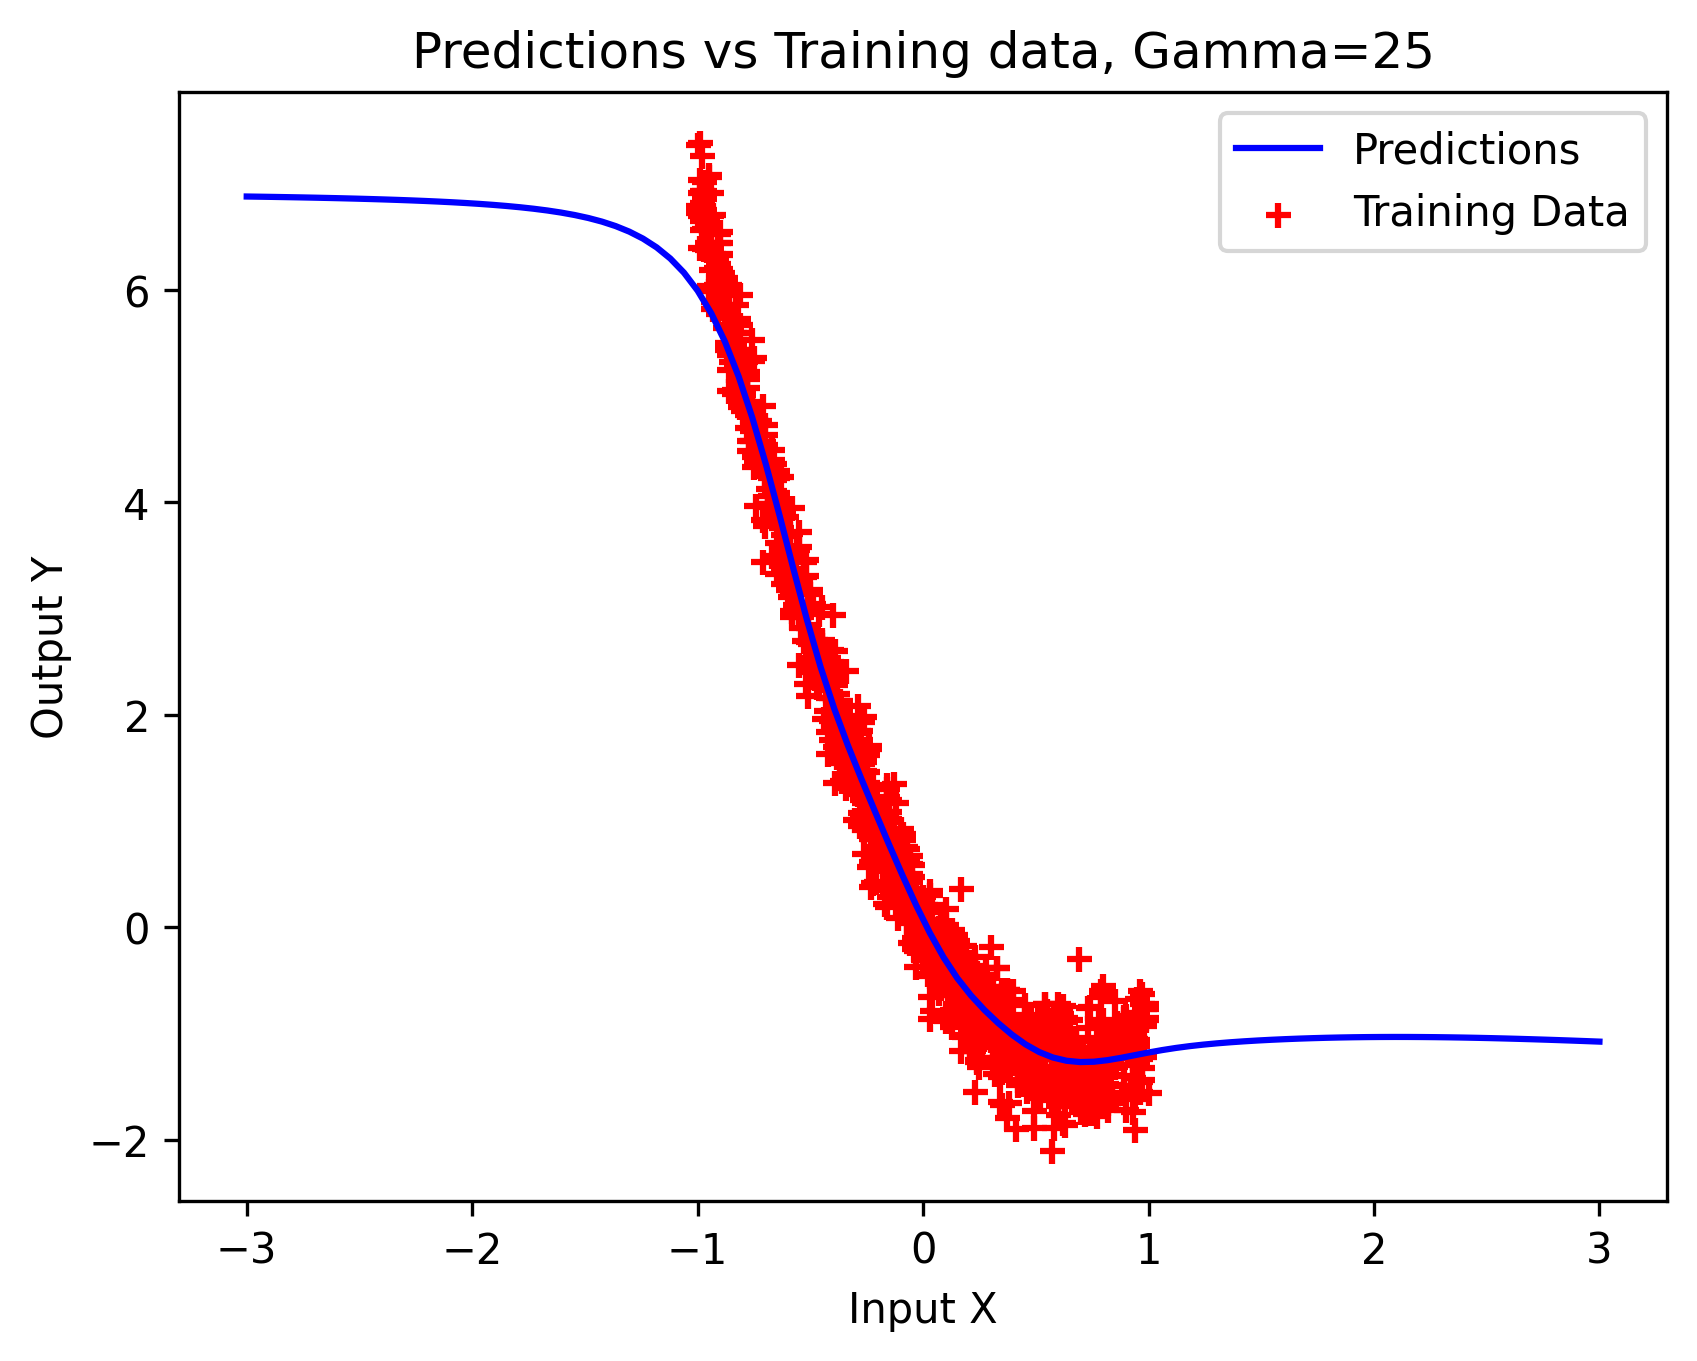
\includegraphics[width=8cm]{ks4.png}}}
\end{figure}
From the figures we can see that as we alter gamma, our predictions fit closer to the training data. This is due to the fact as our gamma grows, the output for our kernel decreases, causing the weights on points closer to the origin point to be decreased, meaning the influence of other points is decreased overall, causing predictions to follow the trend of the data much more closely than when Gamma is low. When Gamma is low such as when Gamma = 1, the influence of other points is much higher so the predictor is much more general hence the slight slope. In comparison when Gamma = 10, our predictions follow the trend of the data much more closely. Concerning the data that's out of range of the training data, KNN isn't good at predicting data that isn't within the range of the training data, hence the nearly straight lines we see when X is less than -1 and greater then 1. 
\\
To get the above graphs, I used the KNGaus function but used the dataset from the link provided.
\subsection{B}
\begin{figure}[h]
\centering
\subfloat[]{{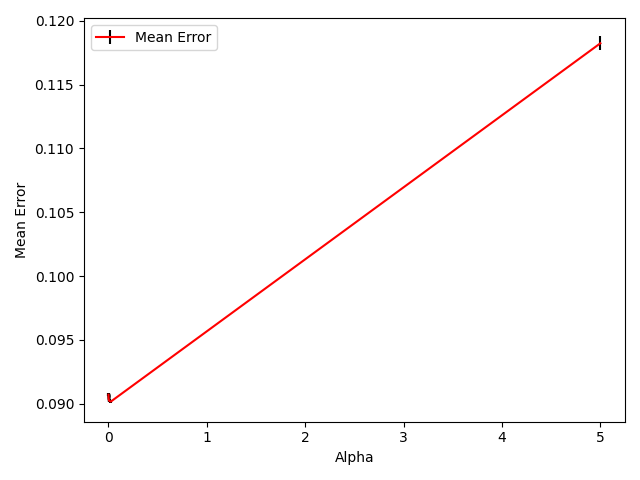
\includegraphics[width=8cm]{cr1.png}}}
\qquad
\subfloat[]{{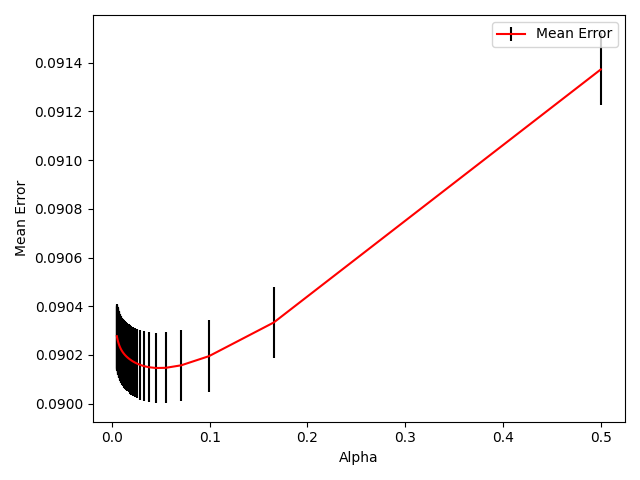
\includegraphics[width=8cm]{cr2.png}}}
\qquad
\end{figure}
I first selected the optimum value of Alpha(1/2C) using cross validation and a default Gamma of 25. I chose 25 at random since I was going to vary the Gamma value afterwards. Initially I used a range of 0.1 to 1000 but as we can see in graph a, larger values of C produced better models so I reduced the range to between 1 and 100. From this I picked a value of 11.102. \\
From the graphs on the next page, we can see that as we increase Gamma, our predictions fit closer and closer to the data with over-fitting being mitigated due to alpha. We can see at higher values of Gamma i.e when Gamma = 25, some over-fitting is beginning to occur as the curve is no longer smooth but jittery as the model is beginning to fit to all the noise in the data. This is due to features introduced by higher values of Gamma causing the predictions to start overfitting the data. With lower values of Gamma, we get much more general predictions as the features introduced by the kernel aren't so extreme so the penalty doesn't need to be as high.
\\ To get the above graphs I created a function called hyper\_pick\_ridge\_gamma(). In this function I created a list of C values to iterate over. For each value of C I did cross validation to get the best value of C. From there I plotted the values of C vs the error to get the best value of C. 
\\ To get the graphs below, I just called the kernel\_ridge function I created and used a static value of C.
\begin{verbatim}
def hyper_pick_ridge_gamma():
    alt_gamma_vals = np.linspace(1, 5, num=25)
    dataframe = read_data()
    mean_list = []
    variance_list = []
    for i in alt_gamma_vals:
        kf = KFold(n_splits=10)
        error_list = []
        global gamma
        gamma = i
        for train, test in kf.split(dataframe):
            x_train, x_test = dataframe.loc[train, 'x'], dataframe.loc[test, 'x']
            y_train, y_test = dataframe.loc[train, 'y'], dataframe.loc[test, 'y']
            model = KernelRidge(alpha=1/(2*11.102), kernel='rbf', gamma=i)
            model.fit(np.array(x_train).reshape(-1, 1), y_train)
            ys = model.predict(np.array(x_test).reshape(-1, 1))
            error_list.append(mean_squared_error(y_test.values, ys))
        error_list = np.array(error_list)
        mean_list.append(error_list.mean())
        variance_list.append(error_list.var())
\end{verbatim}		

\begin{figure}[h]
\centering
\subfloat[Gamma = 0]{{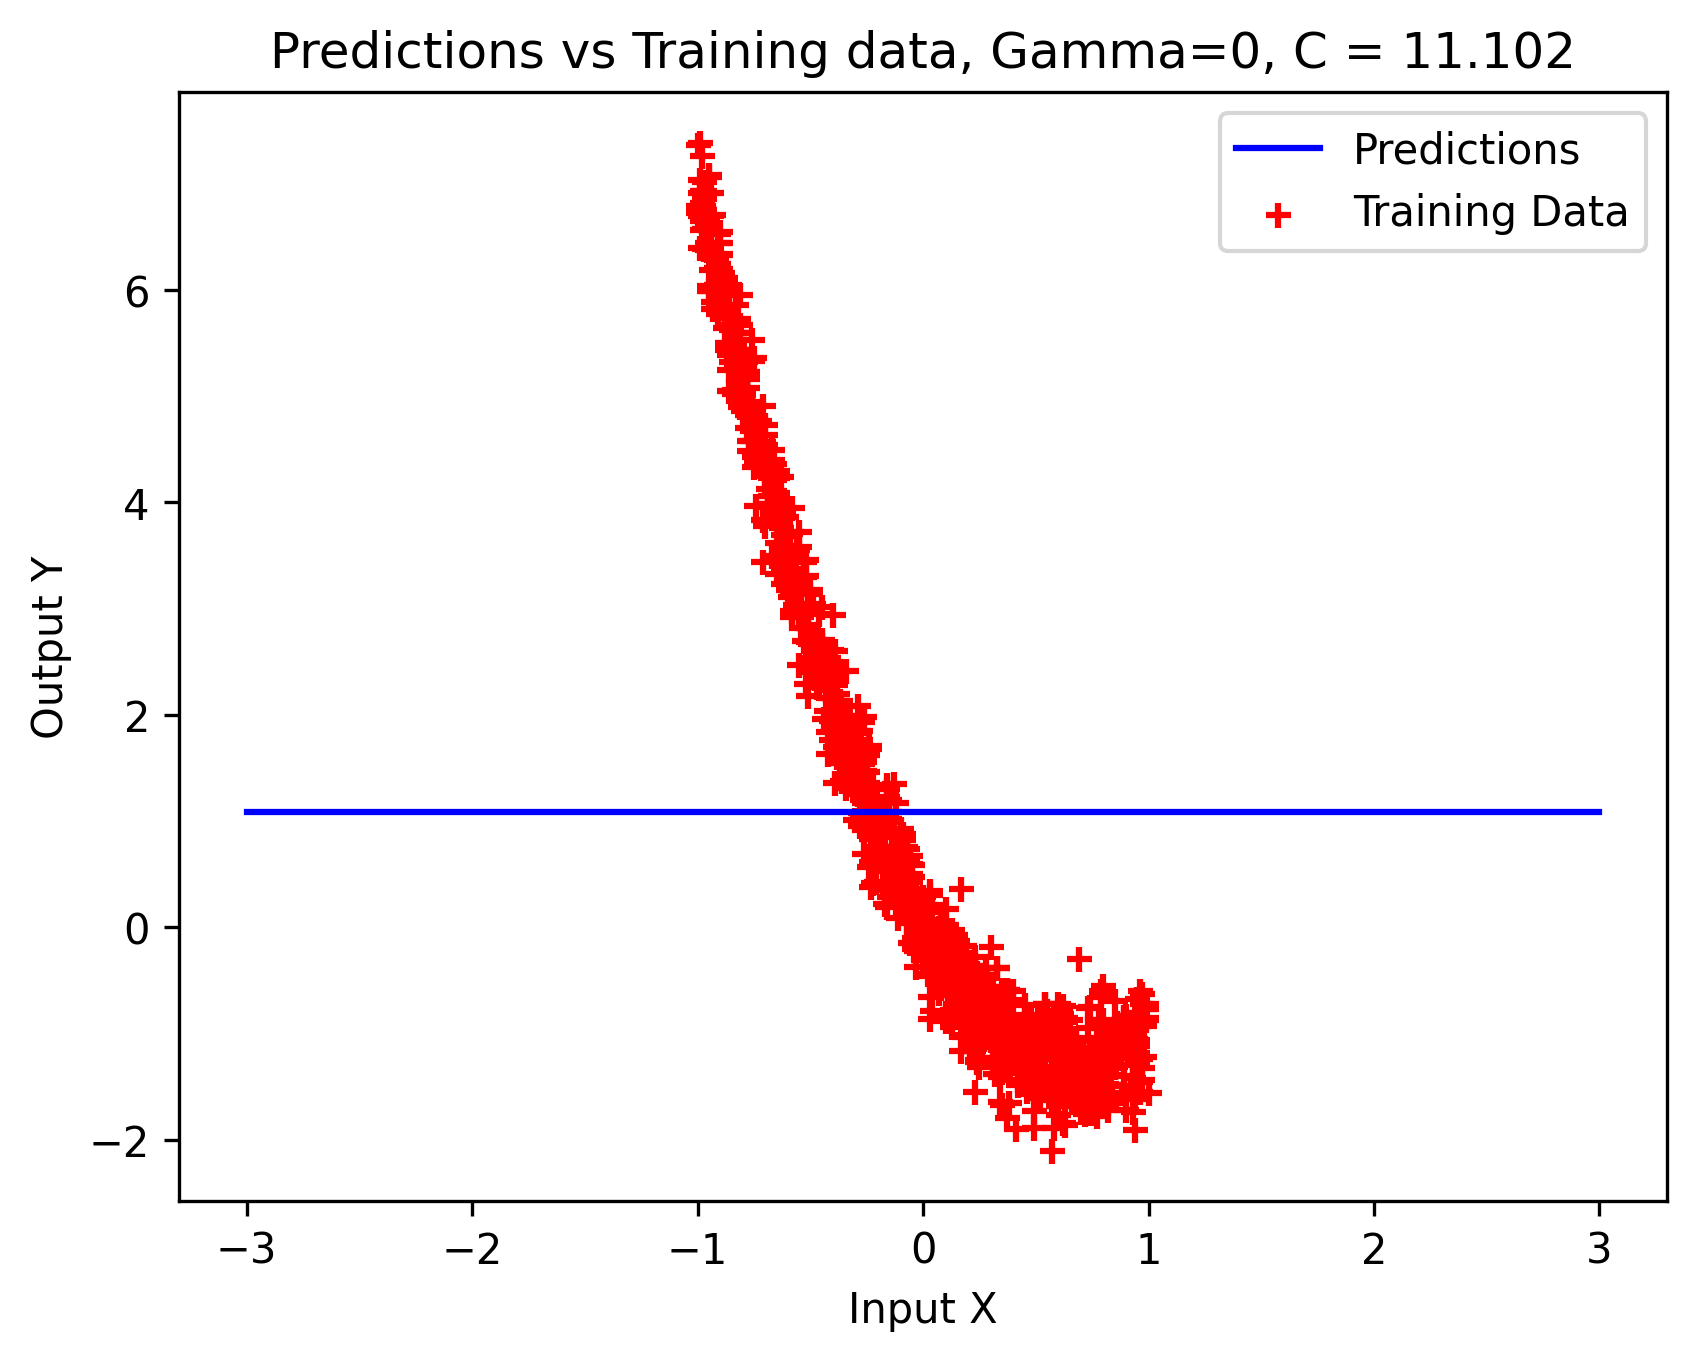
\includegraphics[scale=0.6]{kz0.png}}}
\qquad
\subfloat[Gamma = 1]{{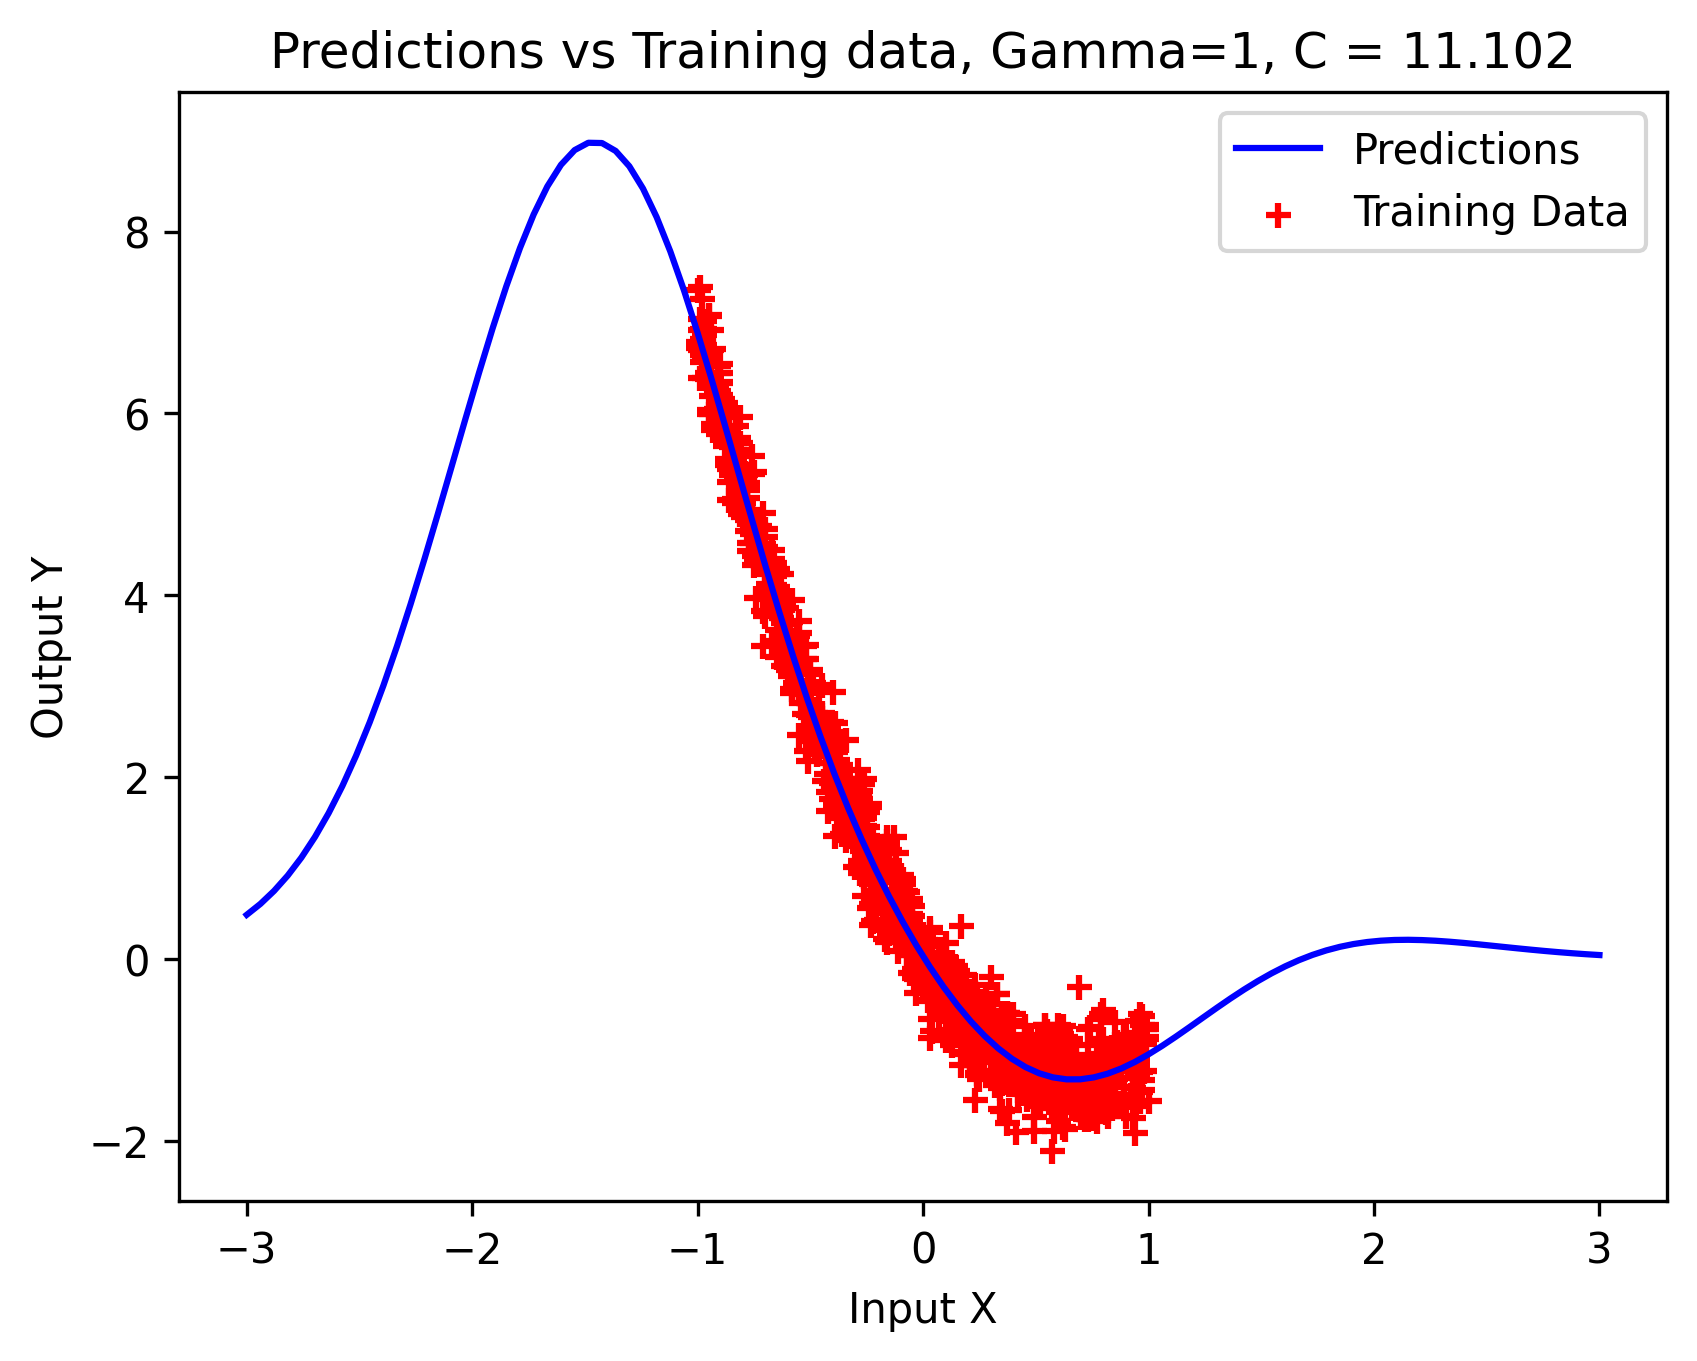
\includegraphics[scale=0.6]{kz1.png}}}
\qquad
\subfloat[Gamma = 5]{{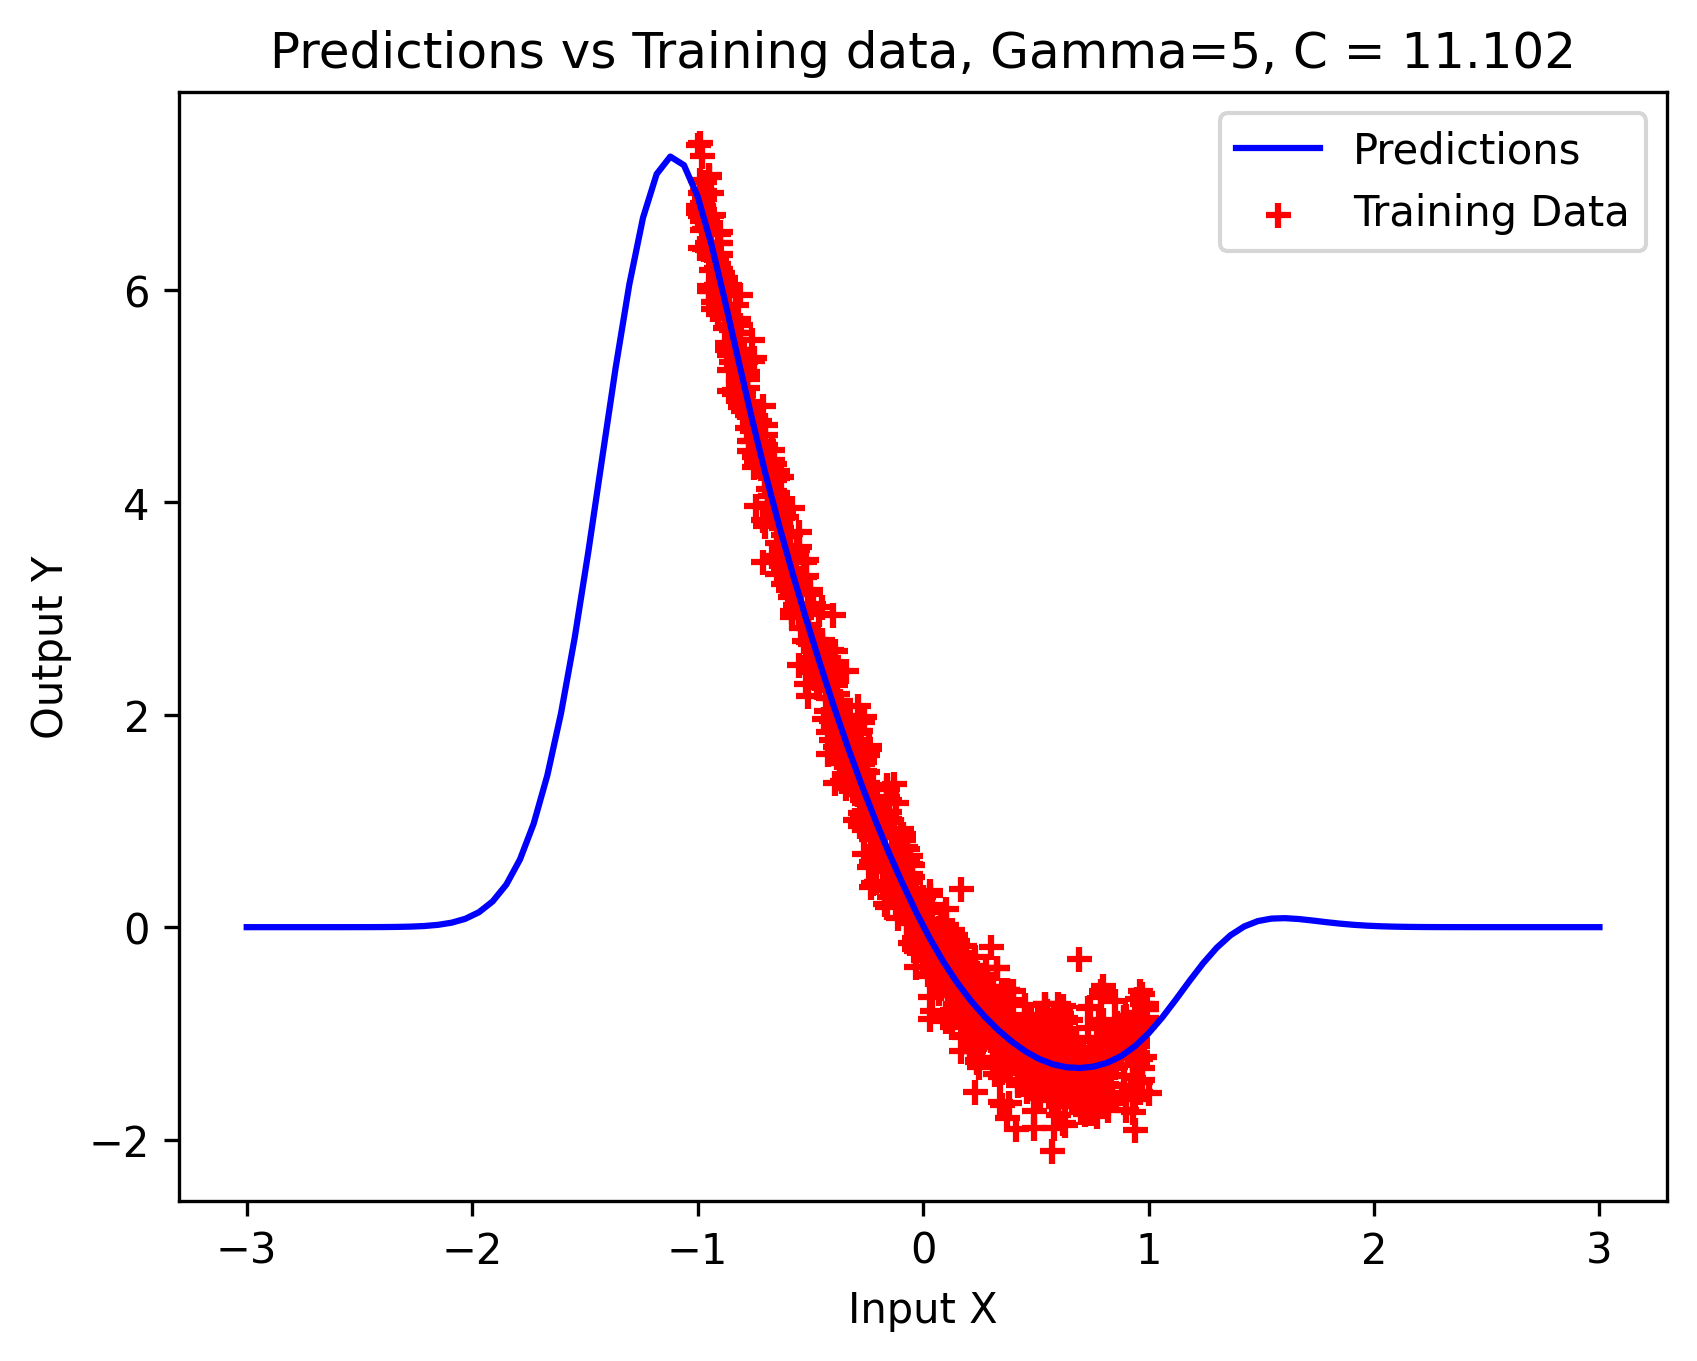
\includegraphics[scale=0.6]{kz2.png}}}
\qquad
\subfloat[Gamma = 10]{{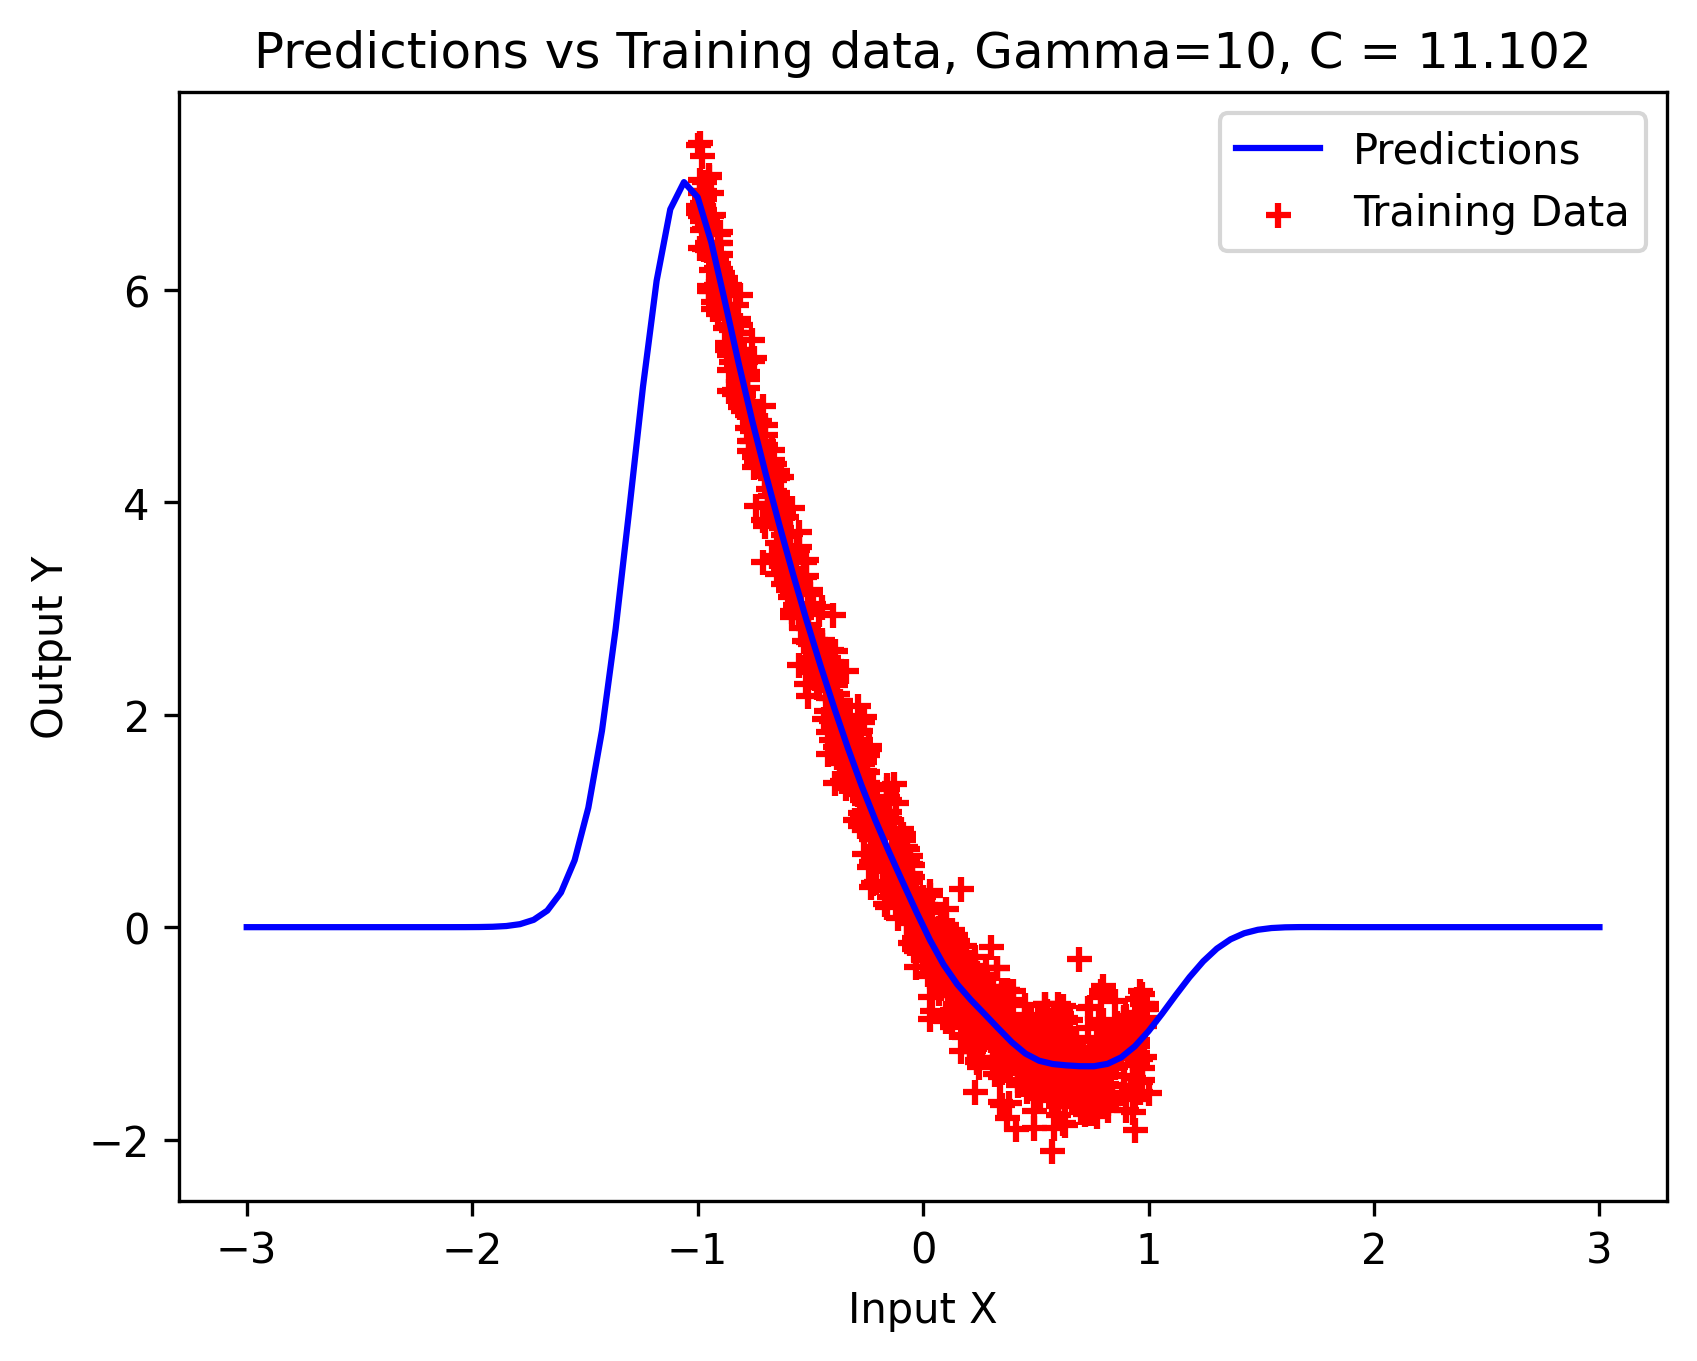
\includegraphics[scale=0.6]{kz3.png}}}
\qquad
\subfloat[Gamma = 25]{{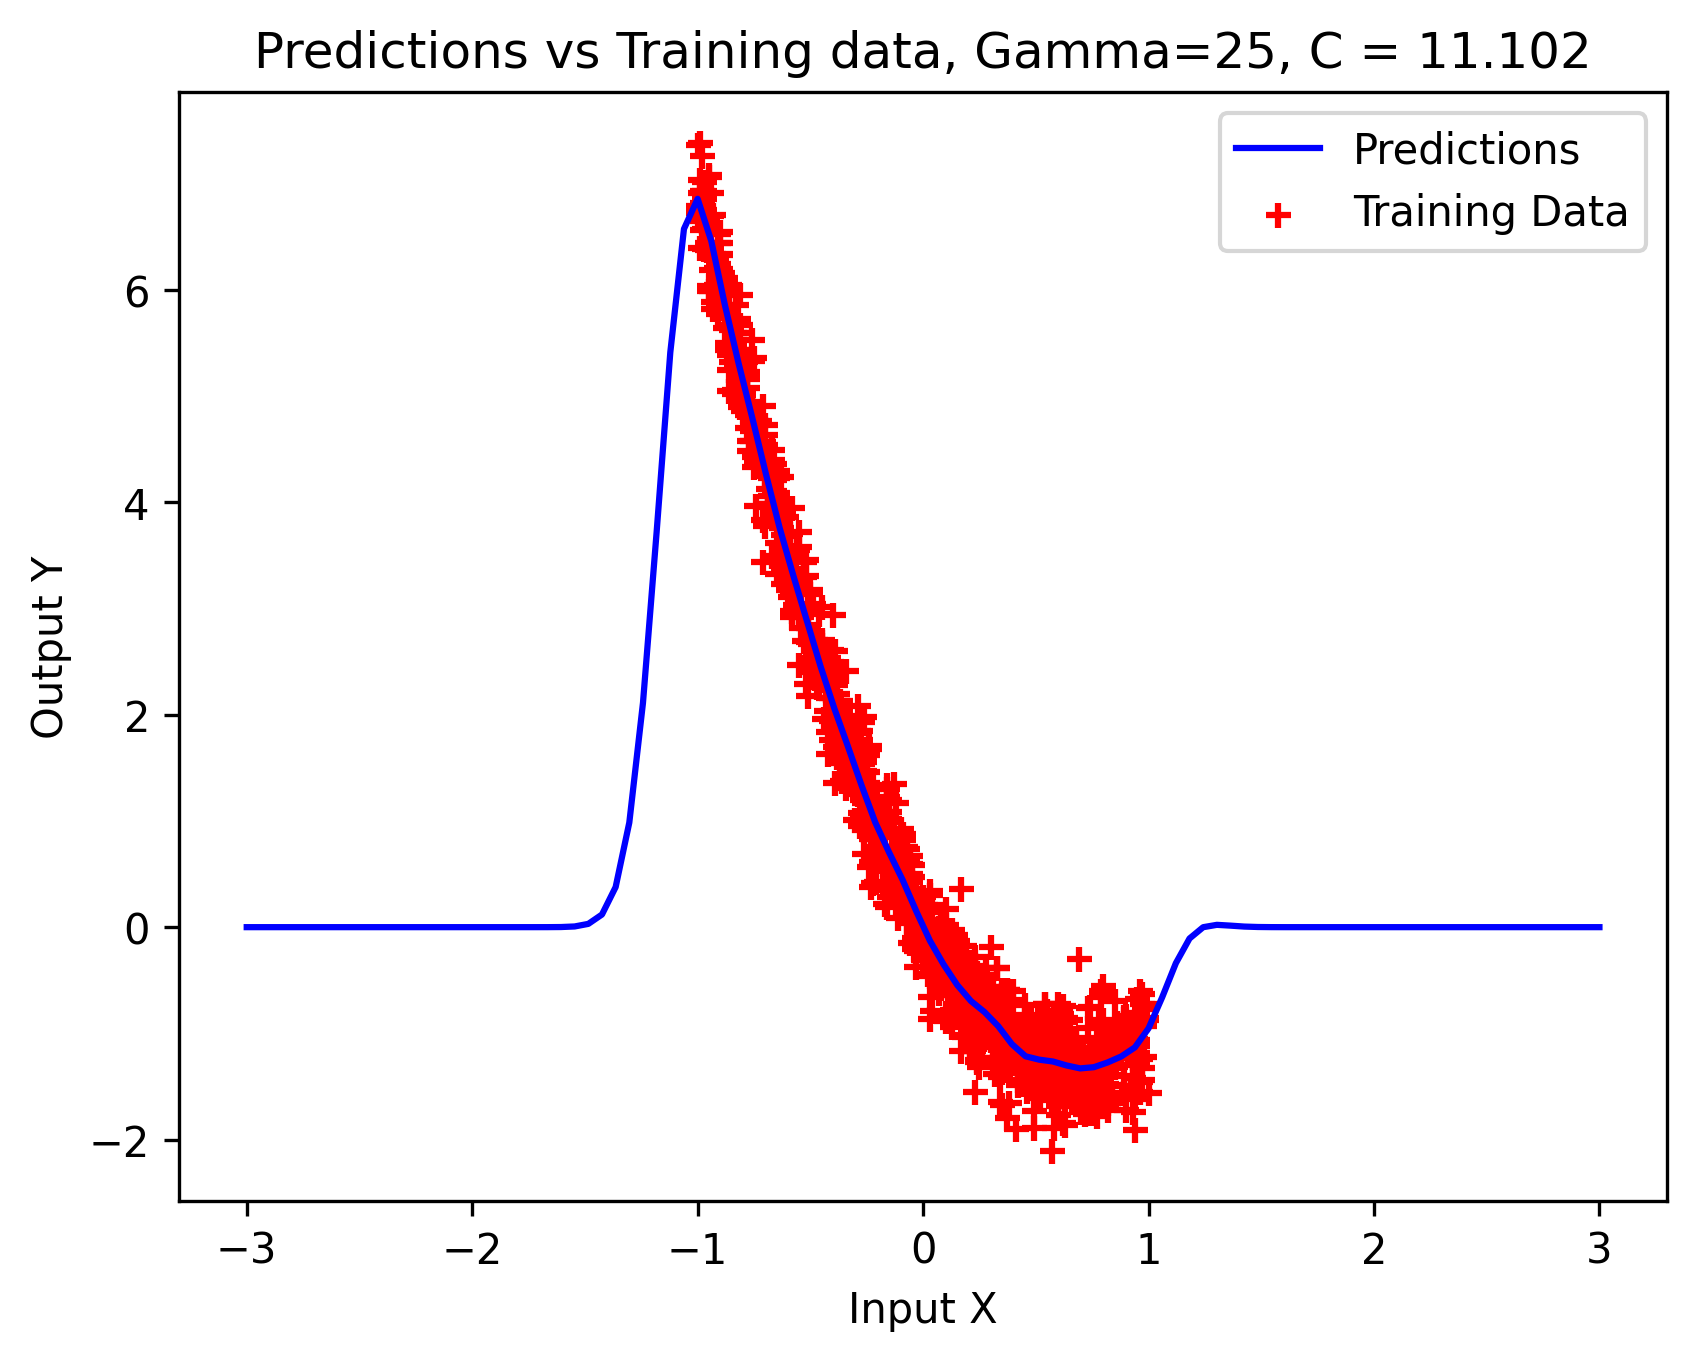
\includegraphics[scale=0.6]{kz4.png}}}
\end{figure}

\clearpage
\subsection{C}
\begin{figure}[h]
\centering
\subfloat[]{{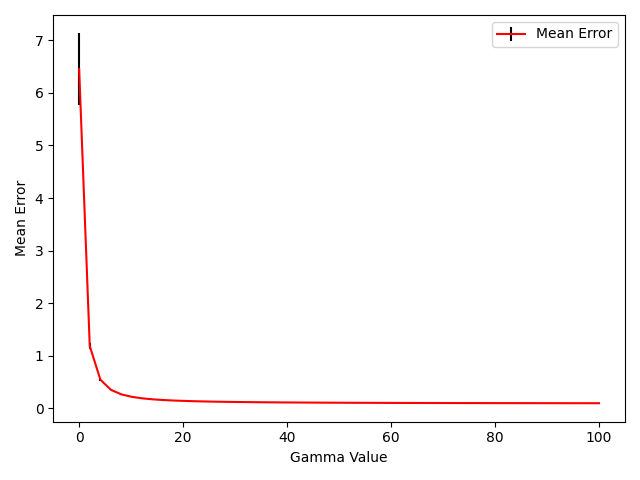
\includegraphics[scale=0.4]{kq1.png}}}
\qquad
\end{figure}
From the above figure, as we increase Gamma, the performance of our model increases also but the amount of error is reducing exponentially also. Based on this it seems using Gamma = 25 should be optimal as having higher values of Gamma only gives us very marginally better models.\\\\ To get the best value of Gamma I used cross validation in a function called hyper\_pick\_knn() The methodology to do it is the same as hyper\_pick\_ridge\_gamma but instead of fitting Kernel Ridge models, I fitted KNNRegressor models instead on predicted on such.
\begin{figure}[h]
\centering
\subfloat[]{{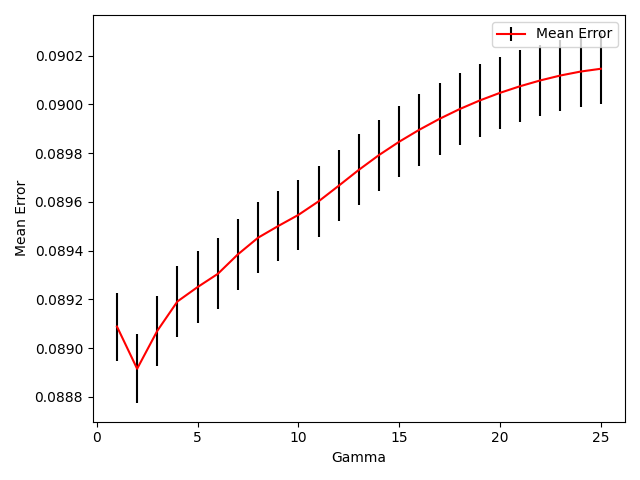
\includegraphics[width=8cm]{fk1.png}}}
\qquad
\subfloat[]{{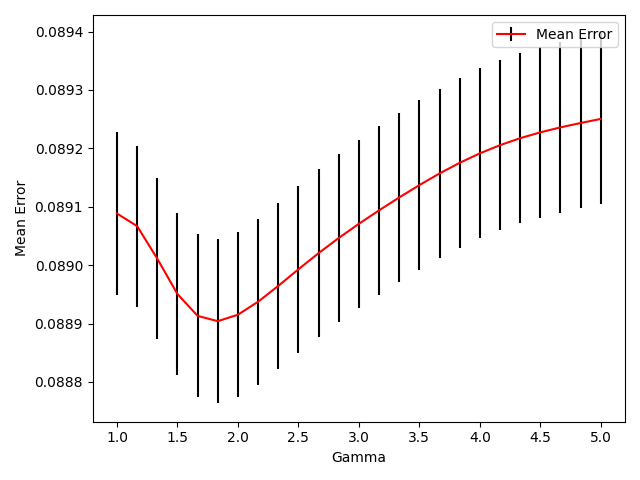
\includegraphics[width=8cm]{fk2.png}}}
\qquad
\end{figure}
As I already selected the best value of C earlier, I hard-coded in the value and then used cross validation to pick Gamma. I started with a range between 0 and 25 but as we can see from figure A, the optimal value is somewhere between 0 and 10 and the mean error even increase as Gamma increases. From figure B, it seems Gamma =1.8 is the optimal value of Gamma.
\clearpage
\begin{figure}[h]
\centering
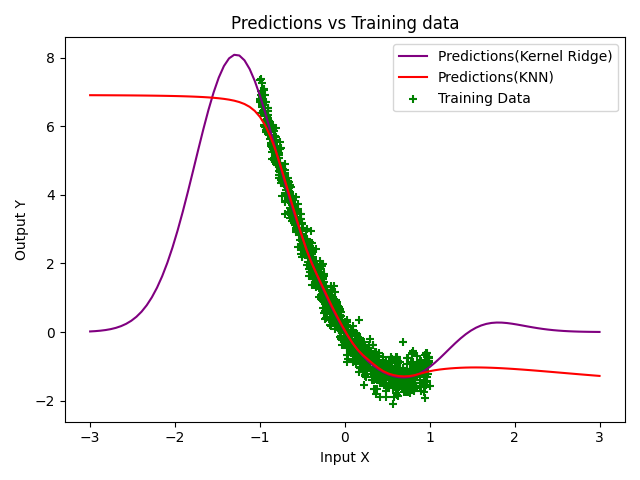
\includegraphics[scale=0.7]{knvkr.png}
\end{figure}
In this figure I plotted the optimal models for both KNN and KRR. From the above graph, we can see that the Kernel Ridge Regression model performs significantly better than out KNN model. The KRR model seems to capture the general trend of the data much better and and also has less error. The KNN model doesn't fully capture all the trends in the data and even misses some of the data in the top of graph completely. The reason the KRR model performs better I believe is because the model is much more general due to having more hyper parameters to tune, both Alpha and Gamma. Due to this we can build much more accurate models in comparison to KNN where we can only tune Gamma. The KRR model seems to be more optimal for this dataset.\\ To get the above graph, I got the best values for each model, created the models in a new function called plotter() and then fitted the models to the data and then predicted on the grid of x inputs. I then plotted the predictions vs the training data.
\section{Code Appendix}
\begin{verbatim}
data = {'x': [-1, 0, 1], 'y': [0, 1, 0]}
df = pd.DataFrame(data)
gamma = 25
gamma_Vals = [0, 1, 5, 10, 25]
c_vals = np.linspace(start=.1, stop=1000, num=50)
grid = np.linspace(start=-3, stop=3, num=100).reshape(-1, 1)


def gaussian_kernel(distances):
    weights = np.exp(- gamma * (distances ** 2))
    return weights / np.sum(weights)


def read_data():
    f = open("week6.txt", "r")
    start = True
    data = {'x': [], 'y': []}
    for i in f:
        if not start:
            i = i.rstrip('\n')
            vals = i.split(",")
            data['x'].append(float(vals[0]))
            data['y'].append(float(vals[1]))
        else:
            start = False
    return pd.DataFrame(data)


def KNGaus():
    dataframe = read_data()
    for i in range(len(gamma_Vals)):
        global gamma
        gamma = gamma_Vals[i]
        model = KNeighborsRegressor(n_neighbors=len(dataframe), weights=gaussian_kernel)
        model.fit(np.array(dataframe['x']).reshape(-1, 1), dataframe['y'])
        ys = model.predict(grid)
        plt.clf()
        plt.scatter(dataframe['x'], dataframe['y'], color='red', marker='+', label='Training Data')
        plt.plot(grid, ys, color='blue', label='Predictions')
        plt.xlabel("Input X")
        plt.ylabel("Output Y")
        plt.title(f'Predictions vs Training data, Gamma={gamma}')
        plt.legend()
        # plt.savefig(f'ks{i}.png', dpi=300, bbox_inches='tight')
        plt.show()


def kernel_Ridge():
    dataframe = read_data()
    # for i in range(len(c_vals)):
    for s in range(len(gamma_Vals)):
            global gamma
            gamma = gamma_Vals[s]
            model = KernelRidge(alpha=1 / (2 * 11.102), kernel='rbf', gamma=gamma)
            model.fit(np.array(dataframe['x']).reshape(-1, 1), dataframe['y'])
            ys = model.predict(grid)
            plt.clf()
            plt.scatter(dataframe['x'], dataframe['y'], color='red', marker='+', label='Training Data')
            plt.plot(grid, ys, color='blue', label='Predictions')
            plt.xlabel("Input X")
            plt.ylabel("Output Y")
            plt.title(f'Predictions vs Training data, Gamma={gamma}, C = {11.102}')
            plt.legend()
            plt.savefig(f'kz{s}.png', dpi=300, bbox_inches='tight')
            plt.show()
            # print(
            #     f'\(\\thetha_0 {round(model.dual_coef_[0], 9)}, thetha_1 {round(model.dual_coef_[1], 9)} , thetha_2 {round(model.dual_coef_[2], 9)}\)')


def hyper_pick_knn():
    alt_gamma_vals = np.linspace(0, 100)
    dataframe = read_data()
    mean_list = []
    variance_list = []
    for i in alt_gamma_vals:
        kf = KFold(n_splits=10)
        error_list = []
        global gamma
        gamma = i
        for train, test in kf.split(dataframe):
            x_train, x_test = dataframe.loc[train, 'x'], dataframe.loc[test, 'x']
            y_train, y_test = dataframe.loc[train, 'y'], dataframe.loc[test, 'y']
            model = KNeighborsRegressor(n_neighbors=len(x_train), weights=gaussian_kernel)
            model.fit(np.array(x_train).reshape(-1, 1), y_train)
            ys = model.predict(np.array(x_test).reshape(-1, 1))
            error_list.append(mean_squared_error(y_test.values, ys))
        error_list = np.array(error_list)
        mean_list.append(error_list.mean())
        variance_list.append(error_list.var())
    plt.clf()
    plt.errorbar(alt_gamma_vals, mean_list, variance_list, label="Mean Error", color='red', ecolor='black')
    plt.xlabel('Gamma Value')
    plt.ylabel('Mean Error')
    plt.legend()
    plt.show()
    print(alt_gamma_vals)
    print(mean_list)


def hyper_pick_ridge_gamma():
    alt_gamma_vals = np.linspace(1, 5, num=25)
    dataframe = read_data()
    mean_list = []
    variance_list = []
    for i in alt_gamma_vals:
        kf = KFold(n_splits=10)
        error_list = []
        global gamma
        gamma = i
        for train, test in kf.split(dataframe):
            x_train, x_test = dataframe.loc[train, 'x'], dataframe.loc[test, 'x']
            y_train, y_test = dataframe.loc[train, 'y'], dataframe.loc[test, 'y']
            model = KernelRidge(alpha=1/(2*11.102), kernel='rbf', gamma=i)
            model.fit(np.array(x_train).reshape(-1, 1), y_train)
            ys = model.predict(np.array(x_test).reshape(-1, 1))
            error_list.append(mean_squared_error(y_test.values, ys))
        error_list = np.array(error_list)
        mean_list.append(error_list.mean())
        variance_list.append(error_list.var())

    plt.clf()
    plt.errorbar(alt_gamma_vals, mean_list, variance_list, label="Mean Error", color='red',
                 ecolor='black')
    plt.xlabel('Gamma')
    plt.ylabel('Mean Error')
    plt.legend()
    plt.show()
    print(c_vals)
    print(mean_list)

def plotter():
    dataframe = read_data()
    global gamma
    gamma = 25
    model1 = KernelRidge(alpha=1/(2*11.102), kernel='rbf', gamma=1.8)
    model2 = KNeighborsRegressor(n_neighbors=len(dataframe), weights=gaussian_kernel)
    model1.fit(np.array(dataframe['x']).reshape(-1, 1), dataframe['y'])
    model2.fit(np.array(dataframe['x']).reshape(-1, 1), dataframe['y'])
    ys1 = model1.predict(np.array(grid).reshape(-1, 1))
    ys2 = model2.predict(np.array(grid).reshape(-1, 1))
    plt.clf()
    plt.scatter(dataframe['x'], dataframe['y'], color='green', marker='+', label='Training Data')
    plt.plot(grid, ys1, color='purple', label='Predictions(Kernel Ridge)')
    plt.plot(grid, ys2, color='red', label='Predictions(KNN)')
    plt.xlabel("Input X")
    plt.ylabel("Output Y")
    plt.title('Predictions vs Training data')
    plt.legend()
    plt.show()

plotter()
\end{verbatim}
\end{document}
